\documentclass[12pt]{amsart}
\usepackage{amsmath,amssymb,url}
\usepackage{geometry} % see geometry.pdf on how to lay out the page. There's lots.
\geometry{a4paper} % or letter or a5paper or ... etc
% \geometry{landscape} % rotated page geometry

%  POSSIBLY USEFULE PACKAGES
%\usepackage{graphicx}
%\usepackage{tensor}
\usepackage{todonotes}
\usepackage{hyperref}

%  NEW COMMANDS
\newcommand{\pder}[2]{\ensuremath{\frac{ \partial #1}{\partial #2}}}
\newcommand{\ppder}[3]{\ensuremath{\frac{\partial^2 #1}{\partial
      #2 \partial #3} } }
\newcommand{\R}{\ensuremath{\mathbb{R}}}

%  NEW THEOREM ENVIRONMENTS
\newtheorem{thm}{Theorem}[section]
\newtheorem{prop}[thm]{Proposition}
\newtheorem{cor}[thm]{Corollary}
\newtheorem{lem}[thm]{Lemma}
\newtheorem{defn}[thm]{Definition}

%  NEW REMARKS
\theoremstyle{remark}
\newtheorem{rmk}[thm]{Remark}


%%%%%%%%%%%%%%% Holm Macros
\def\MM#1{\boldsymbol{#1}}
\newcommand{\pp}[2]{\frac{\partial #1}{\partial #2}} 
\newcommand{\dede}[2]{\frac{\delta #1}{\delta #2}}
\newcommand{\dd}[2]{\frac{\diff #1}{\diff #2}} 
\newcommand{\sothree}{\mathfrak{so}(3)}
% \contract is a differential geometry contraction sign _|
\def\contract{\makebox[1.2em][c]{\mbox{\rule{.6em}
{.01truein}\rule{.01truein}{.6em}}}}
%%%%%%%%%%%%%%%%%%%%%%%%%%%%%%%%%%%%%%%%%%%

%  MATH OPERATORS
\DeclareMathOperator{\SDiff}{SDiff}
\DeclareMathOperator{\GL}{GL}
\DeclareMathOperator{\SO}{SO}
\DeclareMathOperator{\ad}{ad}
\DeclareMathOperator{\Ad}{Ad}
\DeclareMathOperator{\Jet}{Jet}
\DeclareMathOperator{\Orb}{Orb}

%  TITLE, AUTHOR, DATE
\title{Jet vortex methods}
\author{Darryl D. Holm \& Henry O. Jacobs\\ \\
Department of Mathematics\\
Imperial College, London SW7 2AZ, UK}
\date{\today}


\begin{document}

\begin{abstract}
A new singular vortex theory is presented for regularised Euler fluid equations of ideal incompressible flow in the plane. We determine the conditions under which such regularised Euler fluid equations may admit vorticity singularities which are stronger than delta functions, e.g., derivatives of delta functions. We also characterise the Hamiltonian dynamics of the higher-order singular vortices. Applications to the design of numerical methods similar to vortex blob methods are also discussed. 
\end{abstract}

\maketitle

\section{Introduction}
\label{sec:intro}
Vortices are important in hydrodynamics because they are the sources for the incompressible flow field. The vorticity distribution at any instant of time determines both the current state of the flow and its future evolution, for given boundary conditions. This property holds for any Hamiltonian system, and it can indeed be shown that the dynamics of vortices can be usefully expressed in Hamiltonian form. In the vorticity and stream function formulation of an ideal incompressible planar fluid, the evolution of the vorticity distribution $\omega(x,y,t)$ is given by
\begin{align}
  \partial_t \omega + \{\omega,\psi\} := 
  \partial_t \omega + \partial_x \omega  \partial_y \psi
  - \partial_y \omega \partial_x \psi = 0\,, \label{eq:vorticity}
\end{align}
where $\omega = \Delta \psi$ is the vorticity and $\psi$ is the stream function.
The corresponding $(x,y)$ components of the Eulerian velocity field are given by
\begin{align*}
	 (u,v) = (\partial_y \psi , - \partial_x \psi).
\end{align*}

If one is willing to view the vorticity $\omega$ as a distribution, one can consider point vortex solutions.
In particular, point vortices are obtained if one considers the vorticity solution ansatz 
\[\omega(z,t) = \sum_{i} \Gamma_i(t) \delta_{z_i}\,,\]
where $\Gamma_i \in \mathbb{R}$, $z=(x,y) \in \mathbb{R}^2$ and $\delta_{z_i}:=\delta(z-z_i(t))$ is the Dirac delta distribution centered at the point $z_i = (x_i,y_i) \in \mathbb{R}^2$.
Substitution of this ansatz into \eqref{eq:vorticity} yields the following well known finite dimensional system in the form  of Hamilton's canonical equations,
\begin{align}
\begin{cases}
	\frac{d \Gamma}{dt} = 0 \,,\quad  \quad \psi(z,t) = \sum_i  \Gamma_i(t) G(z-z_i(t)) \,, \\
	\frac{dx_i}{dt} = \partial_y \psi(z_i) \,,\quad  \quad \frac{dy_i}{dt} = - \partial_x \psi(z_i)\,,
\end{cases} \label{eq:point_vortex},
\end{align}
where $G(z) =  - (2\pi)^{-1} \ln( \| z \|)$ is the Green's function for the planar Laplacian. 

A point-vortex approximation to a continuous distribution of vorticity is problematic, though, because a point vortex induces a flow velocity which becomes unbounded. However, when the point vortex is smoothed out and made bounded (regularized) the approximation becomes reasonable  \cite{Chorin1973}.

For example, one may consider the regularized form of the vorticity equation given by
choosing a translationally and rotationally invariant smoothing kernel $K_\delta$ of width $\delta$ and defining the regularized vorticity as 
$K_\delta* \omega = \Delta \psi$.
For example, $K_\delta (z) = \exp( - \| z\|^2 / \delta^2)$ is considered in \cite{BealeMajda1985}.
In this case the point vortex ansatz yields \eqref{eq:point_vortex} again, except that the Green's function $G$ is replaced by the kernel
\begin{align}
	G_\delta(z) := K_\delta*G(z) = \frac{1}{4\pi} \left( {\rm Ei}(- \| z \|^2 / \delta^2) - 2\ln ( \| z \|) \right), \label{eq:kernel}
\end{align}
where ${\rm Ei}( \cdot )$ denotes the exponential integral function.
The vorticity kernel $G_\delta$ has no singularity at the origin for $\delta > 0$, and is known as a \textit{vortex blob}.
This system is the starting point for the vortex blob method, introduced in \cite{Chorin1973} (albeit with a different regularization).

The economy of the vortex blob method derives from the property that Dirac delta distributions are hyper-local (i.e. parametrized by position), and the property that the vorticity equation  \eqref{eq:vorticity} admits Dirac delta distributions as solutions.
However, there are many distributions which are localized to a similar degree (e.g. derivatives of delta functions, $\partial_x \delta_{z_i}$).

In this paper, we study the more general vorticity solution ansatz,
\[\omega(z,t) = \sum_{i,m,n} \Gamma_i^{mn}(t) \partial_x^m \partial_y^n \delta_{z_i}\,.\]
We will find that this ansatz yields a closed finite dimensional system which generalizes vortex blobs. We call these new carriers of vorticity \emph{jet vortices}.

\subsection{Main contributions}
\begin{enumerate}
        \item Section \ref{sec:background} briefly reviews the background for vortex methods in fluid modeling.
        \item Section \ref{sec:EOM} derives the equations of motion for point vortices and jet vortices as exact solutions of a regularized vorticity equation. Remark \ref{rmk:conserved} derives the conservation laws for these equations, such as energy, linear momentum, and angular momentum. Other conservation laws are explained in Appendix \ref{sec:symmetries}. The implications of Kelvin's circulation theorem for jet vortices are discussed in Section \S \ref{rmk:Kelvin}. The relation of the resulting closed dynamical systems for jet vortices to the equations of motion for the spatial moments of the vorticity distribution is explained in Remark \ref{rmk:moments}.
        \item Section \ref{sec:numerics} discusses numerical aspects of using jet vortices to model fluid dynamics. Section \ref{sec:grouping} shows how to reduce the number of pairwise interactions, by grouping nearby jet vortices into a single jet vortex of higher order. In Section \ref{sec:approximation}, we spectrally approximate an initial condition using jet vortices and plot the convergence rate. 
        \item   Section \ref{sec:numerical_experiments} presents the results of several numerical experiments involving small numbers of vortices, for $N=1,2$, and $3$.
        	\item Jet vortex dynamics is Hamiltonian. The symplectic and Hamiltonian structure of jet vortex dynamics is presented in Section \S \ref{sec:symplectic}.
\end{enumerate}

\section{Background}
\label{sec:background}
Vortex methods for fluid modeling predate the computer age. They can already be found in a 1931 paper concerning a ``line of discontinuity'' in planar fluid flow \cite{Rosenhead1931}.
At the beginning of their development, the infinite induced velocity at the location of the point vortex cores for Euler flows caused great difficulties, both numerically and theoretically. In fact, the point vortex approach did not produce a competitive numerical method until the 1970s, when the problems related to singularities were overcome by regularizing the singular vortex kernel to form a \emph{vortex blob}.
Stochastic perturbations were further included to model viscosity and the Kutta condition was invoked to create vorticity around boundaries \cite{Chorin1973}.
These three adjustments to the classical vortex method made the method of practical use for realistic fluid flow modeling.
In particular, blob regularization proved much more amenable to analysis. For example, the convergence to solutions of the Navier-Stokes equations was proven in \cite{Hald1979}.
Stronger convergence rates were achieved by judicious choice of vortex kernels.
By convolving the singular vortex kernel with sums of Gaussian smoothing kernels, a sequence of vortex blob kernels with faster and faster convergence rates was found.
In particular, the convergence rate of the $m$th kernel was found to be spectral, and of order $h^{mq}$ for any $q \in (0,1)$ where $h = \delta^q$
is a grid-spacing parameter and $\delta > 0$ is a length scale associated to the smoothing kernel \cite{BealeMajda1982,BealeMajda1985}.

Simultaneously, the symplectic geometry of point vortices was clarified in \cite{MarsdenWeinstein1983}
by invoking Arnold's interpretation of ideal fluids \cite{Arnold1966}.
The findings of \cite{MarsdenWeinstein1983} were developed further in \cite{GayBalmazVizman2012} to handle fluid flow on manifolds with nontrivial homology.
While this theoretical development clarified the geometry of point vortices, vortex blobs were thought to be a numerical ``trick" which violated the geometric interpretation.
However, this thought was banished with the invention of the Euler-$\alpha$ model, a regularized model of ideal fluids with a parameter $\alpha$ representing the typical correlation length of fluctuations away from the mean of a Lagrangian fluid path. In particular, vortex blob solutions associated to a specific kernel serve as \emph{exact} solutions to the Euler-$\alpha$ model \cite{OliverShkoller2001}.
The Euler-$\alpha$ kernel is different from the kernels used in \cite{Chorin1973} and \cite{BealeMajda1985}.
A comparison of the Euler-$\alpha$ kernel to the $m=1$ kernel of \cite{BealeMajda1985} is given in \cite{HolmNitschePutkaradze2006}.

While vortex blobs performed well, they did not capture all of the qualitative richness observed in fluid vorticity dynamics.
In particular, blobs of vorticity in real ideal fluids are known to change shape and deviate from initially circular distributions.
A numerical method is proposed in \cite{Rossi1997,Rossi2005} to capture these shape dynamics by adding
basis functions with non-trivial moments in the study of vortex merger (see for example \cite{MelanderZabuskyMcWilliams1998,DizesVerga2002,MeunierDizesLeweke2005}).
Another distinct model obtained by projection onto a Hermite basis is described in \cite{NagemSandriUminskyWayne2009}.
This projection yielded a finite-dimensional systems which modeled the (truncated) moments of the vorticity of an ideal incompressible fluid.
The derivation of simplified combinatorial formulas invoked by the dynamics of this model were discovered in \cite{UminskyWayneBarbaro2010}
and these formulas have made the method numerically tractable for a large number of moments.

\section{Equations of motion}
\label{sec:EOM}
In this section we derive the equations of motion for the time-dependent parameters which specify the properties of jet vortices.

\subsection{0th order}
At 0th order, one considers the following ansatz for the vorticity
\begin{align}
  \omega(z,t) = \sum_{i} \Gamma_i(t) \delta_{z_i(t)} \label{eq:ansatz 0}
\end{align}
for spatially constant, but potentially time dependent $\Gamma_i(t) \in \R$ for $i$ taking values in some finite set $S$
and where the points $z_i \in \R^2$ are distinct.
The stream function corresponding to this singular solution ansatz for vorticity is 
\begin{align*}
  \psi(z,t) = \sum_{i} \Gamma_i(t) G_\delta (z-z_i(t) )\,.
\end{align*}
Consequently, the induced velocity field is given by
\begin{align}
\begin{cases}
  u(z,t) = \sum_{i} \Gamma_i(t) \partial_y G_\delta (z-z_i(t) ) \\
  v(z,t) = - \sum_{i} \Gamma_i(t) \partial_x G_\delta (z-z_i(t) )
\end{cases} \label{eq:u 0}
\end{align}
%
An image of the stream function and the flow field induced by a single vortex is depicted in Figure \ref{fig:zero}

\begin{figure}[h] %  figure placement: here, top, bottom, or page
   \centering
   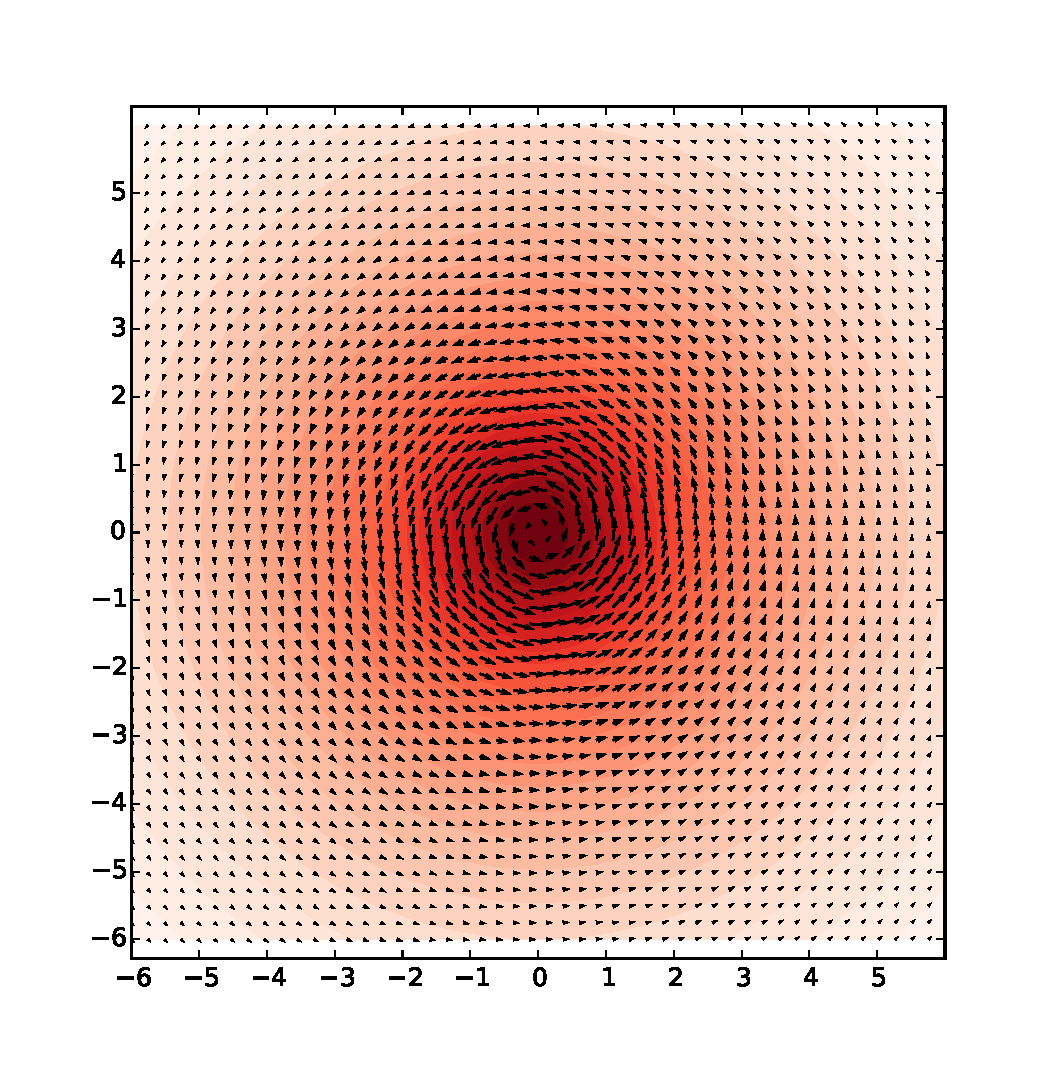
\includegraphics[clip,trim=0.6in 0.5in 0.6in 0.6in,width=0.3\textwidth]{./images/zero.pdf} 
   \caption{A 0th order jet vortex with $z = 0$ and $\Gamma=1$, using the kernel $G_\delta$ of equation \eqref{eq:kernel}. This form of the kernel produces one of the vortex blobs presented in \cite{BealeMajda1985}.}
   \label{fig:zero}
\end{figure}

We seek equations of motion for the $\Gamma_i(t)$'s and $z_i(t)$'s
such that the velocity field \eqref{eq:u 0} satisfies the vorticity equation \eqref{eq:vorticity}.
In the calculations, we will suppress the notation for time dependence of the dynamical quantities.

The 0-jet vortex formulas \eqref{eq:ansatz 0} and \eqref{eq:u 0} imply the following expressions for the terms appearing in the vorticity equation \eqref{eq:vorticity},
\begin{align}
  \partial_t \omega = \sum_{i} \frac{d \Gamma_i}{dt} \delta_{z_i} 
  - \Gamma_i \frac{dx_i}{dt} \partial_x \delta_{z_i}
  - \Gamma_i \frac{dy_i}{dt} \partial_y \delta_{z_i}.
  \label{eq:time derivative}
\end{align}
and
\begin{align*}
  u \partial_x \omega = \sum_{i} u \Gamma_i \partial_x \delta_{z_i}.
\end{align*}
Here the term $u \partial_x \delta_{z_i}$ should be interpreted
using the basic theory of distributions \cite{Hormander2003}.
Upon applying formula \eqref{eq:func times partial delta} in Appendix
\ref{sec:distributions} we find
\begin{align}
  u \partial_x \omega = \sum_{i} \Gamma_i u(z_i) \partial_x \delta_{z_i} - \partial_x u(z_i) \delta_{z_i}. \label{eq:u term}
\end{align}
Similarly, we find
\begin{align}
    v \partial_y \omega = \sum_{i} \Gamma_i v(z_i) \partial_y \delta_{z_i} - \partial_y v(z_i) \delta_{z_i}. \label{eq:v term}
\end{align}
Substitution of \eqref{eq:time derivative},\eqref{eq:u term},
and \eqref{eq:v term} into \eqref{eq:vorticity} now yields
\begin{align*}
\frac{d \Gamma_i}{dt} \delta_{z_i} 
  - \Gamma_i \frac{dx_i}{dt} \partial_x \delta_{z_i}
  - \Gamma_i \frac{dy_i}{dt} \partial_y \delta_{z_i}
  + \Gamma_i u(z_i) \partial_x \delta_{z_i} - \partial_x u(z_i) \delta_{z_i}\\
  \quad +\, \Gamma_i v(z_i) \partial_y \delta_{z_i} - \partial_y v(z_i) \delta_{z_i} =  0.
\end{align*}
This is a linear combination of the independent distributions $\delta_{z_i},\partial_x\delta_{z_i}$ and $\partial_y \delta_{z_i}$.
Thus, to satisfy the equation, the coefficients of each of them must vanish independently.
The vanishing of the coefficient of $\delta_{z_i}$ yields
\begin{align*}
  \frac{d\Gamma_i}{dt} = \partial_x u(z_i) + \partial_y v(z_i).
\end{align*}
Hence, as the flow is divergence free, we find
\begin{align*}
  \frac{d\Gamma_i}{dt} = 0.
\end{align*}
The vanishing of the coefficients $\partial_x \delta_{z_i}$ and $\partial_y \delta_{z_i}$ yields
\begin{align}
  \frac{dx_i}{dt} = u(z_i) \,,\quad  \quad \frac{dy_i}{dt} = v(z_i).
  \label{eq:point motion}
\end{align}
When $x_i(t),y_i(t)$ and $\Gamma_i(t)$ satisfy these equations of motion, the vorticity equation \eqref{eq:vorticity} admits the ansatz \eqref{eq:ansatz 0} as a solution.

\subsection{1st order}
Consider now the following first order jet vortex solution ansatz for the vorticity
\begin{align}
  \omega(t) = \sum_{i} \Gamma_i(t) \delta_{z_i} 
  + \Gamma_i^x(t) \partial_x \delta_{z_i}
  + \Gamma_i^y(t) \partial_y \delta_{z_i}\label{eq:ansatz 1} \,,
\end{align}
for spatially constant dynamical variables $\Gamma_i(t),\Gamma_i^x(t),\Gamma_i^y(t) \in \R$ for $i = 1,\dots,N$.
The stream function in this case is given by the convolution
\begin{align*}
  &\psi(z,t) = G_\delta * \omega = \int G_\delta(z - \tilde{z}) \omega(\tilde{z}) d \tilde{z} \\
  &\quad = \sum_{i} \Gamma_i(t) G_\delta (z-z_i(t) )  + \Gamma_i^x(t) \partial_x G_\delta( z - z_i(t))  + \Gamma_i^y(t) \partial_y G_\delta( z- z_i(t))
  \,.
\end{align*}
The corresponding velocity field takes the form
\begin{align}
\begin{array}{ll}
  u(z,t) &= \sum_{i} \Gamma_i(t) \partial_yG_\delta (z-z_i(t) ) + \Gamma_i^x(t) \partial_{xy} G_\delta( z-z_i(t))\\
  &\qquad + \Gamma_i^y(t) \partial_y^2 G_\delta( z-z_i(t)) \,,\\ \\
  v(z,t) &= \sum_{i} -\Gamma_i(t) \partial_x G_\delta (z-z_i(t) ) - \Gamma_i^x(t) \partial_x^2 G_\delta( z-z_i(t)) \\
  &\qquad - \Gamma_i^y(t) \partial_{xy} G_\delta( z-z_i(t))\,.
\end{array}
\label{eq:u 1}
\end{align}
As an example, the flow field of the 1st order jet vortex with $\Gamma = 0,\Gamma^x = 1,\Gamma^y=1$ is shown in Figure \ref{fig:one}.

\begin{figure}[h] %  figure placement: here, top, bottom, or page
   \centering
   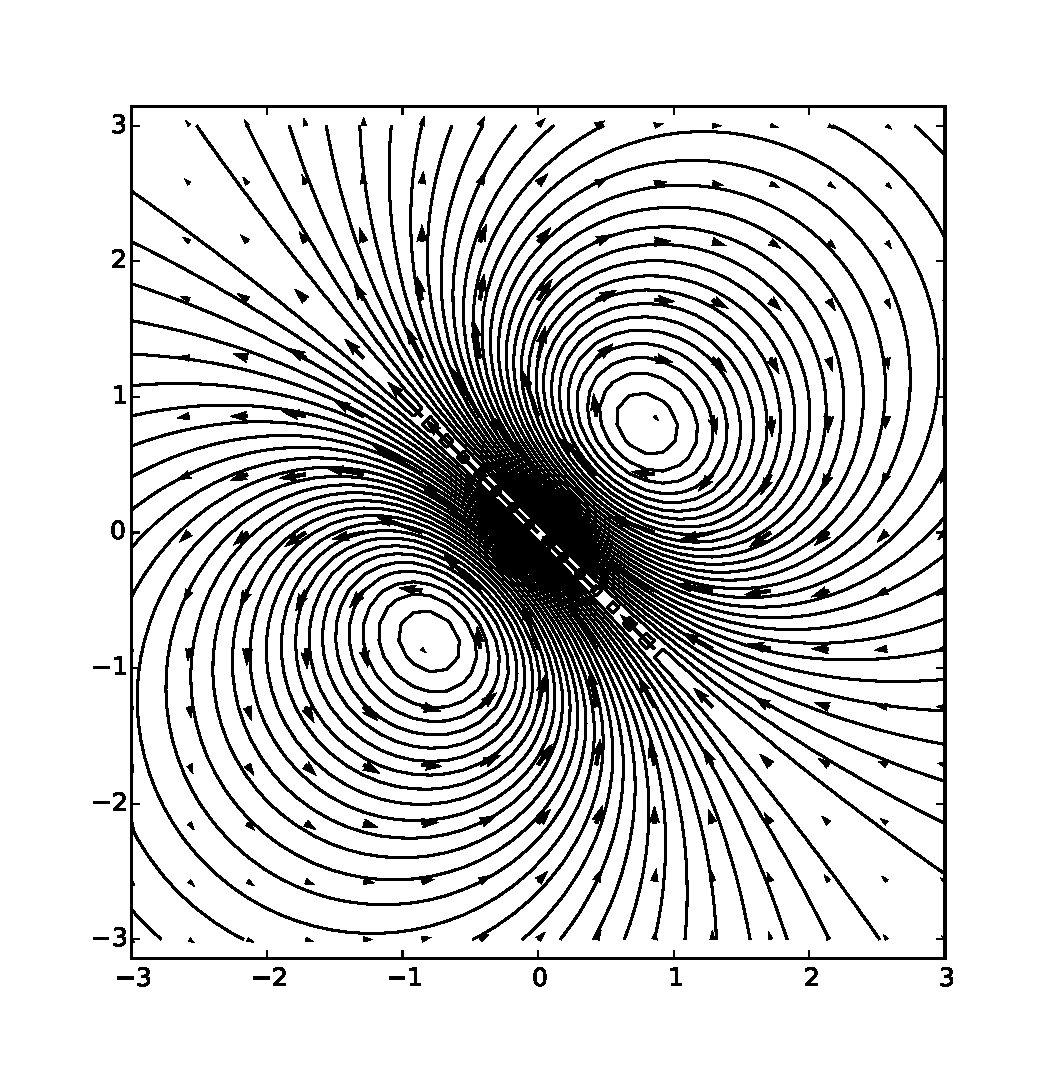
\includegraphics[clip,trim=0.6in 0.5in 0.6in 0.6in,width=0.4\textwidth]{./images/one.pdf} 
   \caption{The flow field around a 1st order jet vortex with $\Gamma = 0,\Gamma^x = 1,\Gamma^y=1$ has a dipole pattern.}
   \label{fig:one}
\end{figure}

We seek equations of motion for the $\Gamma_i(t)$'s and $z_i(t)$'s of 1st order jet vortex
such that the velocity field \eqref{eq:u 1} satisfies the vorticity equation \eqref{eq:vorticity}.
For the calculations, we will suppress the explicit notation for time dependence of the various dynamical quantities.
We then find
\begin{align*}
  \partial_t \omega = \sum_{i} & \frac{d \Gamma_i}{dt} \delta_{z_i} 
  - \Gamma_i \frac{dx_i}{dt} \partial_x \delta_{z_i}
  - \Gamma_i \frac{dy_i}{dt} \partial_y \delta_{z_i} \\
  &+\frac{d \Gamma_i^x}{dt} \partial_x\delta_{z_i} 
  - \Gamma_i^x \frac{dx_i}{dt} \partial_x^2 \delta_{z_i}
  - \Gamma_i^x \frac{dy_i}{dt} \partial_{xy} \delta_{z_i} \\
  &+\frac{d \Gamma_i^y}{dt} \partial_y \delta_{z_i} 
  - \Gamma_i^y \frac{dx_i}{dt} \partial_{xy} \delta_{z_i}
  - \Gamma_i^y \frac{dy_i}{dt} \partial_y^2 \delta_{z_i}
\end{align*}
and
\begin{align*}
  u \partial_x \omega = \sum_{i} u \Gamma_i \partial_x \delta_{z_i}
  + u \Gamma_i^x \partial_x^2 \delta_{z_i} 
  + u \Gamma_i^y \partial_{xy} \delta_{z_i}.
\end{align*}
Invoking \eqref{eq:func times partial delta} (see Appendix
\ref{sec:distributions}) enables a rearrangement of the previous equation to
obtain
\begin{align*}
  u \partial_x \omega &= \sum_{i} \Gamma_i \Big( u(z_i) \partial_x \delta_{z_i} - \partial_x u(z_i) \delta_{z_i} \Big) \\
   &+\Gamma_i^x \Big(u(z_i) \partial_x^2 \delta_{z_i} 
   - 2\partial_x u(z_i) \partial_x \delta_{z_i}
   + \partial_x^2u(z_i) \delta_{z_i} \Big) \\
   &+\Gamma_i^y \Big( u(z_i) \partial_{xy} \delta_{z_i} 
   - \partial_x u(z_i) \partial_y \delta_{z_i} 
   - \partial_y u(z_i) \partial_x \delta_{z_i} 
   + \partial_{xy}u(z_i) \delta_{z_i}\Big).
\end{align*}
Similarly, we find
\begin{align*}
    v \partial_y \omega &= \sum_{i} \Gamma_i \Big( v(z_i) \partial_y \delta_{z_i} - \partial_y v(z_i) \delta_{z_i} \Big) \\
   &\quad + \Gamma_i^x \Big(v(z_i) \partial_{xy} \delta_{z_i} 
   - \partial_x v(z_i) \partial_y \delta_{z_i}
   - \partial_y v(z_i) \partial_x \delta_{z_i}
   + \partial_{xy} v(z_i) \delta_{z_i} \Big) \\
   &\quad + \Gamma_i^y \Big( v(z_i) \partial_{y}^2 \delta_{z_i} 
   - 2\partial_y v(z_i) \partial_y \delta_{z_i} 
   + \partial_{y}^2v(z_i) \delta_{z_i} \Big).
\end{align*}
Substitution of these expressions into \eqref{eq:vorticity} yields
the vanishing of
a linear combination of the distributions
$\delta_{z_i},\partial_x\delta_{z_i},\partial_y \delta_{z_i}, \partial_x^2 \delta_{z_i},
 \partial_{xy} \delta_{z_i}$, and $\partial_y^2 \delta_{z_i}$.
As each of these distributions is linearly independent
of the others (assuming the $z_i$'s are distinct),
their coefficients must vanish independently.
The vanishing of the coefficient of $\delta_{z_i}$ yields
the equation
\begin{align*}
  \frac{d\Gamma_i}{dt} = \partial_x u(z_i) + \partial_y v(z_i)
  + \partial_x^2 u(z_i) + \partial_{xy} v(z_i)
  + \partial_{xy} u(z_i) + \partial_y^2 v(z_i)
\end{align*}
Again, as the flow is divergence free we find
\begin{align*}
  \frac{d\Gamma_i}{dt} = 0.
\end{align*}
The vanishing of the coefficients of $\partial_x^2 \delta_{z_i}$ yields
\begin{align*}
  \Gamma_i^x \left( u(z_i) - \frac{dx_i}{dt} \right) = 0.
\end{align*}
Similarly, by looking at the coefficient of $\partial_y^2 \delta_{z_i}$
we find
\begin{align*}
  \Gamma_i^y \left( v(z_i) - \frac{dy_i}{dt} \right) = 0.
\end{align*}
Assuming $\Gamma_i^x$ and $\Gamma_i^y$ are non-zero we
obtain \eqref{eq:point motion} again.\footnote{
  After we obtain dynamics under this assumption
  we may drop the assumption by continous extension.
  The resulting extension yields the $0$th order
  jet vortex dynamics.
}

Finally, the vanishing of the coefficients $\partial_x \delta_{z_i}$ and $\partial_y \delta_{z_i}$ yields
\begin{align*}
  \frac{d\Gamma^x_i}{dt} = \Gamma_i^x \partial_x u(z_i) + \Gamma_i^y \partial_y u(z_i) \\
  \frac{d\Gamma^y_i}{dt} = \Gamma_i^x \partial_x v(z_i) + \Gamma_i^y \partial_y v(z_i)
\end{align*}
The vorticity equation \eqref{eq:vorticity} admits the ansatz \eqref{eq:ansatz 1} as a solution when $x_i(t),y_i(t)$ and the $\Gamma_i(t)$'s satisfy these equations of motion

\subsection{$N$th order}
Consider the following $N$th order jet vortex ansatz for the vorticity,
\begin{align}
  \omega(z,t) = \sum_{i \in S} \sum_{m+n \leq N} \Gamma^{mn}_i(t) \partial_x^m \partial_y^n \delta_{z_i} \,,
  \label{eq:ansatz N}
\end{align}
for spatially constant dynamical variables $\Gamma^{mn}_i(t) \in \R$ for $i \in S$.
The stream function is 
\begin{align*}
  \psi(z,t) = \sum_{i, m+n \leq N} \Gamma^{mn}_i(t) \partial_x^m \partial_y^n G_\delta (z-z_i(t) )
\,.\end{align*}
The corresponding velocity field is given by
\begin{align}
\begin{cases}
  u(z,t) = \sum_{i \in S,m+n \leq N} \Gamma^{mn}_i(t) \partial_x^m \partial_y^{n+1} G_\delta (z-z_i(t) )
  \,, \\
  v(z,t) = - \sum_{i \in S, m+n \leq N} \Gamma^{mn}_i(t) \partial_x^{m+1} \partial_y^n G_\delta (z-z_i(t) )\,.
\end{cases} \label{eq:u N}
\end{align}

\begin{figure}[h] %  figure placement: here, top, bottom, or page
   \centering
   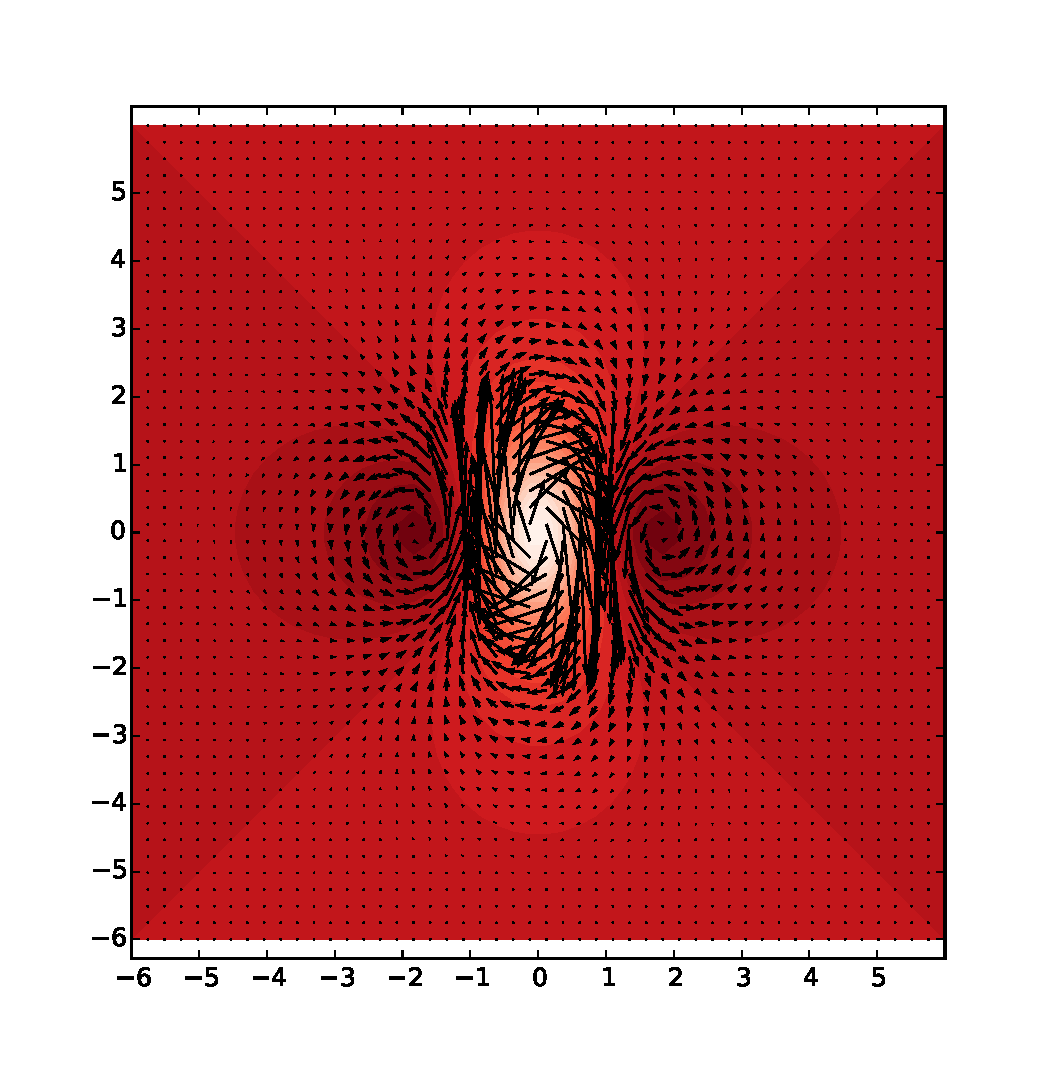
\includegraphics[clip,trim =1in 1in 1in 1in,width=0.3\textwidth]{./images/two_xx.pdf} 
   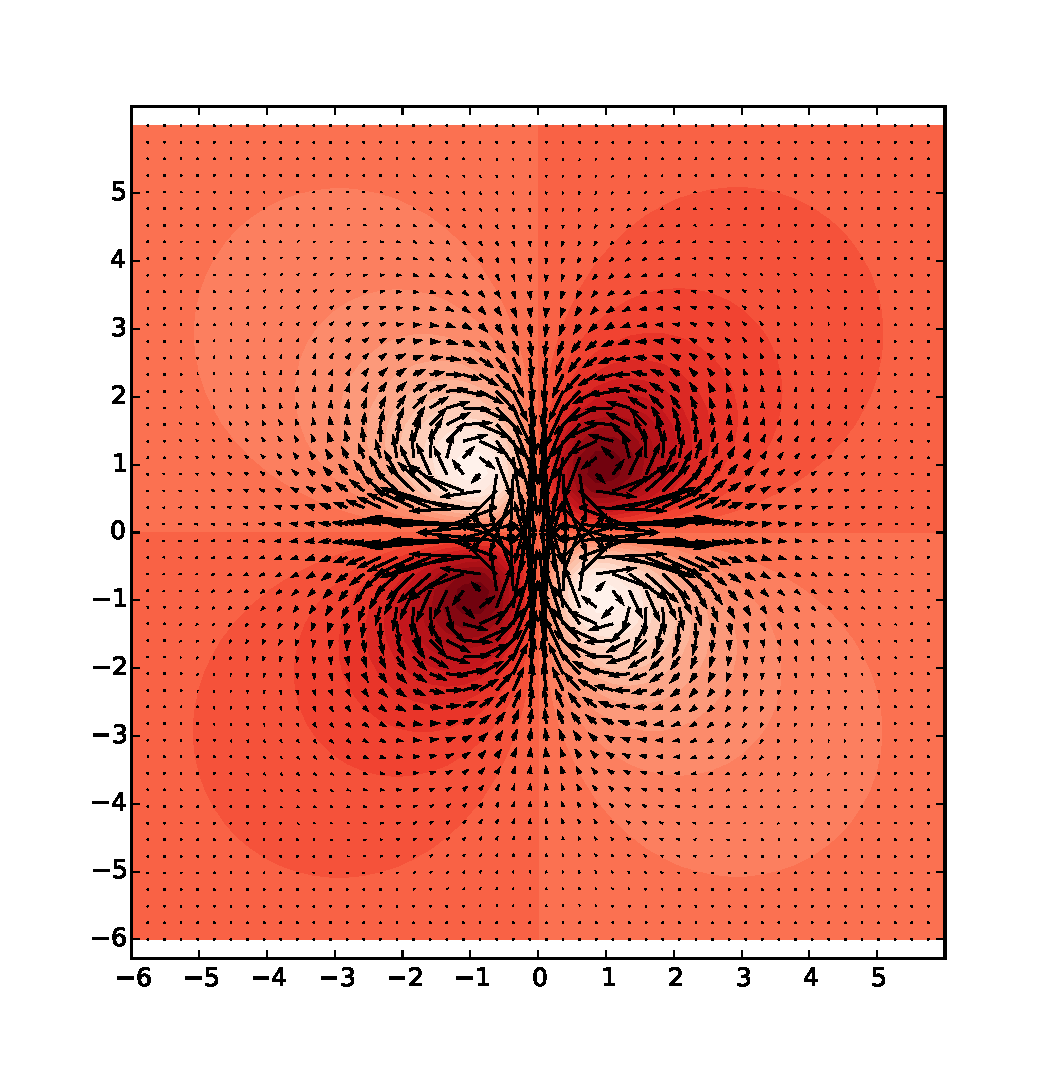
\includegraphics[clip,trim =1in 1in 1in 1in,width=0.3\textwidth]{./images/two_xy.pdf} 
   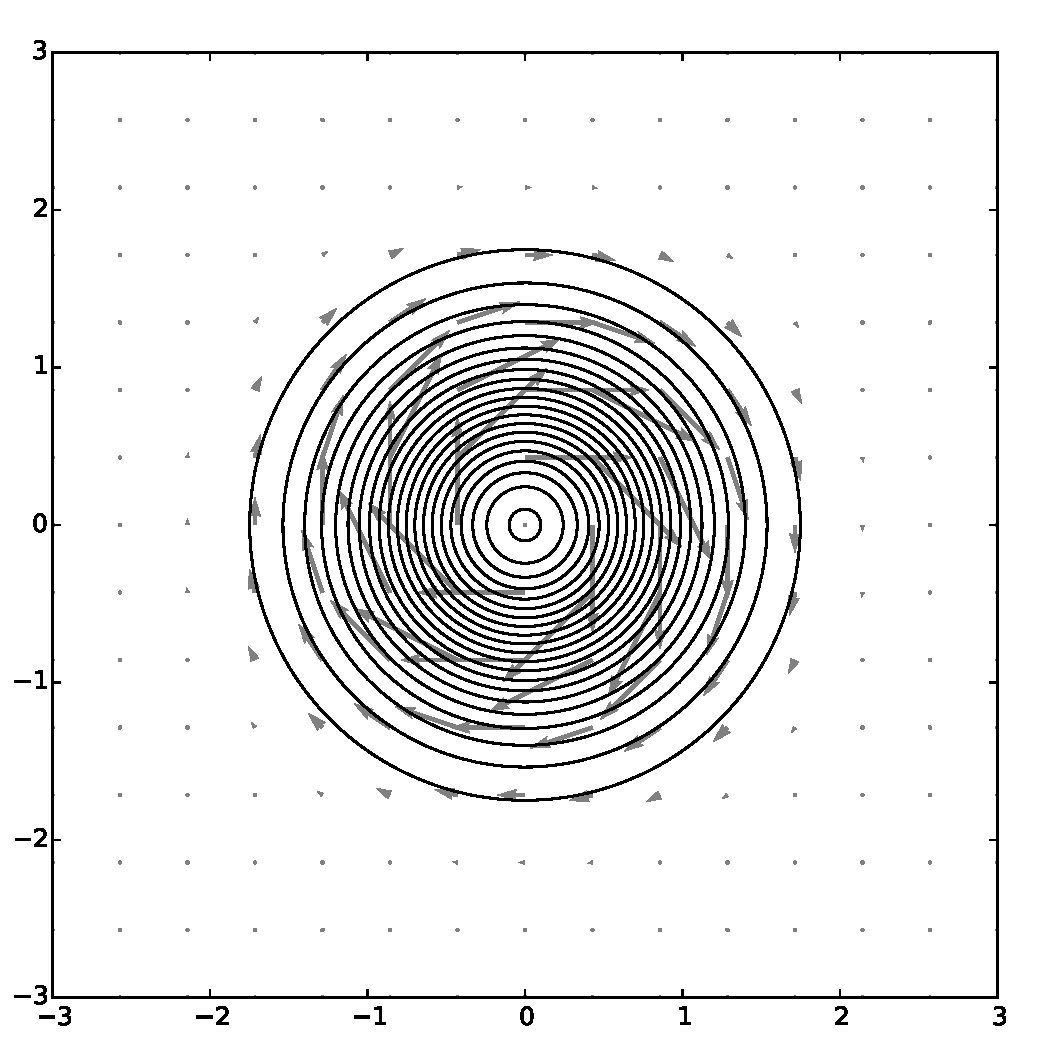
\includegraphics[clip,trim =1in 1in 1in 1in,width=0.3\textwidth]{./images/two_xx_yy.pdf} 
   \caption{Various second order jet vortices with $\Gamma^{00} = \Gamma^{1,0} = \Gamma^{0,1} = 0$.}
   \label{fig:second}
\end{figure}

We seek equations of motion for the $\Gamma^{mn}_i(t)$'s and $z_i(t)$'s
such that the velocity field \eqref{eq:u N} satisfies the vorticity equation \eqref{eq:vorticity}.
In the following calculations, we will not show the explicit time dependence of the dynamical variables.


We now find
\begin{align*}
  \partial_t \omega =	
  \sum_{
  	\substack{
		i \in S \\
		m+n \leq N}}
  	\frac{d \Gamma_i^{mn}}{dt} \partial_x^m \partial_y^n \delta_{z_i} - \Gamma_i^{mn} \frac{dx_i}{dt} \partial_{x}^{m+1} \partial_y^{n} \delta_{z_i}
	- \Gamma_i^{mn} \frac{dy_i}{dt} \partial_{x}^{m} \partial_y^{n+1} \delta_{z_i}\,,
\end{align*}
and
\begin{align*}
  u \partial_x \omega = 
  \sum_{
  	\substack{
		i \in S \\
		m+n \leq N}}
   u \Gamma_i ^{mn}\partial_x^{m+1} \partial_y^n \delta_{z_i}\,.
\end{align*}
By invoking \eqref{eq:func times partial delta} (see Appendix
\ref{sec:distributions}) we can rearrange the previous equation to
obtain
\begin{align*}
  u \partial_x \omega &=
  \sum_{
  	\substack{
		i \in S \\
		m+n \leq N}}
	\Gamma_i^{mn} (-1)^{m+n+1} \sum_{\ell,k} (-1)^{\ell + k} \binom{m+1}{\ell} \binom{n}{k} \partial_x^{\ell} \partial_y^k u(z_i) \partial_x^{m+1-\ell} \partial_y^{n-k} \delta_{z_i}.
\end{align*}
Similarly, we find
\begin{align*}
  v \partial_y \omega &=
  \sum_{
  	\substack{
		i \in S \\
		m+n \leq N}}
	\Gamma_i^{mn} (-1)^{m+n+1} \sum_{\ell,k} (-1)^{\ell + k} \binom{m}{\ell} \binom{n+1}{k} \partial_x^{\ell} \partial_y^k v(z_i) \partial_x^{m-\ell} \partial_y^{n+1-k} \delta_{z_i}.
\end{align*}
Substitution of these expressions into \eqref{eq:vorticity} yields
the vanishing of a linear combination of the distributions
$\partial_x^m \partial_y^n \delta_{z_i}$
for $m+n \leq N+1$.
Since each of these distributions is linearly independent
of the others (assuming the $z_i$'s are distinct),
their individual coefficients must each vanish independently.
Assuming sufficiently many of the $\Gamma_i^{m,n}$'s are non-zero 
for $m+n = N$ we recover \eqref{eq:point motion}.\footnote{
  As before, after we obtain dynamics for the $\Gamma$'s under this assumption
  we may drop the assumption by continuous extension.
  The resulting extension yields the $0$th order
  jet vortex dynamics.
}
The vanishing of the coefficient of $\delta_{z_i}$ yields
\begin{align*}
	\frac{d\Gamma^{0,0}_i}{dt} + \sum_{0 < m+n \leq N} \Gamma^{m,n} ( \partial_x^{m+1}\partial_y^n u(z_i) + \partial_x^{m}\partial_y^{n+1} v(z_i) ) = 0.
\end{align*}
As $u$ is divergence free this equation reduces to
\begin{align*}
	\frac{d \Gamma^{0,0} }{dt} = 0\,.
\end{align*}

For $\ell+k \leq N$ the vanishing of the coefficient of $\partial_{\ell,k} \delta_{z_i}$ yields
\begin{align*}
 \frac{d\Gamma_i^{\ell k}}{dt} = (-1)^{\ell + k}
  \sum_{
    \substack{
      m > \ell \\
      n > k \\
      n+m \leq p}
    }\Gamma_i^{mn} \Bigg[  \binom{n}{k} \binom{m}{\ell-1} \partial_{m-\ell+1,n-k} u^x(z_i) \\
   + \binom{n}{k-1} \binom{m}{\ell} \partial_{m-\ell,n-k+1} u^y(z_i)  \Bigg]
\end{align*}
Again, we have found equations of motion for the $z_i(t)$'s and the $\Gamma_i(t)$'s.
The vorticity equation \eqref{eq:vorticity} admits the $N$th order jet vortex ansatz for the vorticity in \eqref{eq:ansatz N} as a solution when the $z_i(t)$'s and the $\Gamma_i(t)$'s satisfy these equations of motion.

\begin{rmk} \label{rmk:conserved}
  We will find that the following quantities are conserved under the evolution:%\\ \vspace{1em}
  % FOR INCREASING THE SPACING IN THE TABULAR ENVIRONMENT
%\def\arraystretch{1.5}%  1 is the default, change whatever you need
%  \begin{tabular}{|c|c|}
%  	\hline
%	  Linear momentum & $J_{lin} = \sum_i ( \Gamma_i^{0,1} - \Gamma^{0,0}_i y_i , \Gamma^{0,0}_i x_i -\Gamma^{1,0}_i )$ \\
%	  \hline
%	  Angular momentum & ${\bf J}_{\rm ang} = \sum_i \frac{\Gamma^{0,0}_i}{2} (x_i^2 + y_i^2) - \Gamma_i^{1,0} x_i - \Gamma_i^{0,1} y_i + \Gamma_i^{2,0} + \Gamma_i^{0,2}$ \\
%	  \hline
%	  Energy & $E = \sum_{m,n,\ell,k,i} (-1)^{m+n+\ell +k} \Gamma^{mn}_i \Gamma_j^{\ell k} \partial_{m+\ell}^x \partial_{n+k}^y G(z_i-z_j)$ \\
%	  \hline
%  \end{tabular}\\
  \begin{align*}
	  {\bf J}_{\rm ang} &= \sum_i \frac{\Gamma^{0,0}_i}{2} (x_i^2 + y_i^2) - \Gamma_i^{1,0} x_i - \Gamma_i^{0,1} y_i + \Gamma_i^{2,0} + \Gamma_i^{0,2} \,, \\
	  {\bf J}_{\rm lin} &= \sum_i ( \Gamma_i^{0,1} - \Gamma^{0,0}_i y_i , \Gamma^{0,0}_i x_i -\Gamma^{1,0}_i ) \,, \\
	  E &= \sum_{m,n,\ell,k,i} (-1)^{m+n+\ell +k} \Gamma^{mn}_i \Gamma_j^{\ell k} \partial_{m+\ell}^x \partial_{n+k}^y G(z_i-z_j)\,.
  \end{align*}
  The first two quantities, ${\bf J}_{\rm ang}$ and ${\bf J}_{\rm lin}$, are momenta derived from Noether's theorem for the rotational and translational symmetries of the fluid.
  In section \ref{sec:symplectic} we will characterize the jet vortex dynamics as Hamiltonian systems and show that the linear and angular momentum serve as symplectic momentum maps. (See Appendix \ref{sec:symmetries} for the derivations.)
\end{rmk}

\begin{rmk} \label{rmk:Kelvin}
	Let $\vec{u} = (u,v)$ be a time-dependent vector field which satisfies \eqref{eq:vorticity}.
	The flow of $\vec{u}$ is the diffeomorphism, $\Phi_t: \mathbb{R}^2 \to \mathbb{R}^2$,
	which sends particle labels at time $0$ to their positions at time $t$.
	If $\omega_t$ is the vorticity at time $t$ then $\omega_t( \Phi_t(z) ) = \omega_0$ is constant in time.
	This conservation law can be seen as a corollary of Kelvin's circulation theorem.
	As a consequence, the quantity
	\begin{align*}
		J(t) := \int \omega_t( \Phi_t(z) ) f(z) dz
	\end{align*}
	is constant in time for any $f \in C^\infty(\R^2)$.
	By applying the change of variables formula and invoking the
	incompressibility condition, $\det(D\Phi) = 1$, we find
	\begin{align*}
		J(t) = \int \omega_t( z) f(\Phi_t^{-1}(z)) dz.
	\end{align*}
	This form of writing $J(t)$ makes sense when $\omega_t$ is a distribution.
	As a result, we find that for a vorticity of the form \eqref{eq:ansatz N} the quantity
	\begin{align}
		J(t) = \sum_{
			\substack{
				i \in S \\
				m+n \leq N
			}
		} \Gamma_i^{mn} (-1)^{m+n} \partial_x^m\partial_y^n( f \circ \Phi_t^{-1}) |_{z = z_i(t)} \label{eq:conserved_circulation}
	\end{align}
	is conserved for any $f \in C^\infty(\R^2)$.
	While this conservation law holds for all functions, $f$, we do not obtain infinitely many conserved
	quantities when $\omega_t$ satisfies the jet vortex ansatz and $S$ is finite.
	This is because the expression on the right hand side only depends on the $N$-jet of $f$ at $z_i(0) \equiv \Phi_t^{-1}(z_i(t) )$,
	as is illustrated by the Fa\`a di Bruno formula.
	We will not display the Fa\`a di Bruno formula here because it requires nearly a page of notational definitions before to writing it down
	\cite{ConstantineSavits1996,Jacobs2014b}.
	Nonetheless, by computing the cardinality of jet spaces, we would obtain ${\rm card}(S) \frac{ N(N+1)}{2}$ independent conserved quantities
	as a result of \eqref{eq:conserved_circulation}.
	These conserved quantities can be interpreted as a finite dimensional manifestation of the conservation of circulation.
\end{rmk}

\begin{rmk}\label{rmk:moments}
	The $(a,b)^{\rm th}$ moment of the vorticity centered around the vortex position $(x_i,y_i) \in \R^2$ is given by
	\begin{align*}
		\mu^{ab}_i := \int (x-x_i)^a (y-y_i)^b \omega dxdy\,.
	\end{align*}
	If $\omega$ satisfies the jet vortex ansatz \eqref{eq:ansatz N} then
	\begin{align*}
		\mu^{ab}_i = \sum_{
			\substack{
				j \in S \\
				m \leq a ,
				n \leq b
			}
		}
		(-1)^{m+n} \frac{a! b!}{(a-m)!(b-n)!} \Gamma_j^{mn} (x_j - x_i)^{a-m} (y_j - y_i)^{b-n}\,,
	\end{align*}
	for $a+b \leq N$ and $i \in S$.
	Given the points $z_i \in S$, one can write the moments in terms of the circulation
	strengths, the $\Gamma$'s.
	For the moment $\mu_i^{ab}$ with $a+b \leq N$ with $a,b \in \mathbb{N}$
	we may invert this relationship to write $\Gamma_i^{mn}$ as a function of these moments.
	Invoking the equation of motion for the $\Gamma$'s and substituting the identity between the $\Gamma$'s
	and the $\mu$'s
	would yield a closed dynamical system for the $\mu$'s.
	That the equations of motion for the moments forms a closed system at order $N$
	is in contrast to other methods for deriving dynamical systems for moments
	\cite{UminskyWayneBarbaro2010, NagemSandriUminskyWayne2009,GibbonsHolmTronci2008a,GibbonsHolmTronci2008b}
	where a projection must be invoked in order to form a closed system.
\end{rmk}

\section{Numerical Aspects}
\label{sec:numerics}
In this section we discuss various numerical aspects of using jet vortices to model fluid dynamics.
We will present an algorithm for constructing an initial condition of jet vortices from a given stream
function and the procedure for grouping sets of lower order jet vortices into higher order ones.

\begin{rmk}
A full convergence proof is well beyond the scope of this article,
which merely introduces the concept of jet vortices.
Nonetheless, convergence can be quickly verified by observing the convergence proof of the standard vortex blob method.
The convergence of the standard vortex blob method begins by initializing a regular grid of vortex blobs
and observing convergence as the grid spacing vanishes.
In \S \ref{sec:approximation} we will obtain an approximation scheme for the initial condition.
Under this approximation scheme, the order 1 and higher circulation coefficients will vanish as the 
grid resolution vanishes (assuming the initial condition is sufficiently smooth).
Consequently, the jet vortex blob approximation and the standard vortex blob method will converge to the same limit.
As the standard vortex blob method converges to the solutions of the Euler equation, we also obtain convergence for the jet vortex blob approximation.
At the moment we do not know if the jet vortex blob method converges faster (in space and time) than the vortex blob method.
However, we will show in Section \S \ref{sec:approximation} that jet vortices provide an improved approximation in space.
\end{rmk}

\subsection{Grouping and reduction of pairwise computations}
\label{sec:grouping}

Let us consider the vorticity distribution
\begin{align*}
	\omega = \Gamma_1 \delta_{z_1} + \Gamma_2 \delta_{z_2}\,.
\end{align*}
If $z_1$ and $z_2$ are close, we can define the quantities $\bar{z} = (z_1+z_2)/2$ and $\delta z = z_1 - z_2 $ to obtain the approximation
\begin{align*}
	\int \omega(z) f(z)dz &= \Gamma_1 f(z_1) + \Gamma_2 f(z_2) \\
		&= \Gamma_1 \left( f(\bar{z}) + \partial_x f(\bar{z}) \cdot \frac{\delta x}{2} + \partial_y f(\bar{z}) \cdot \frac{\delta y}{2}  \right)\\
		&\quad + \Gamma_2 \left( f(\bar{z}) - \partial_x f(\bar{z}) \cdot \frac{\delta x}{2} - \partial_y f(\bar{z}) \cdot \frac{\delta y}{2}  \right) + o( h ) 
\end{align*}
where $h = \| \delta z \|$.
Therefore the distribution
\begin{align*}
	\tilde{\omega} = \Gamma \delta_{\bar{z}} + \Gamma^x \partial_x \delta_{\bar{z}} + \Gamma^y \partial_y \delta_{\bar{z}}
\end{align*}
with 
\begin{align*}
	\Gamma = \Gamma_1 + \Gamma_2 \quad,\quad \Gamma^x = \frac{\delta x}{2} (\Gamma_2 -\Gamma_1) \quad,\quad \Gamma^y = \frac{\delta y}{2} (\Gamma_2 -\Gamma_1)
\end{align*}
serves as a $o(h)$ approximation of $\omega$ in the sense of distributions.
Moreover, the stream function $\tilde{\psi} := G_\delta * \tilde{\omega}$ is an $o(h)$ approximation of $\psi := G_\delta * \omega$ in the traditional sense of analysis on functions.

We have just described the first case of grouping two $N$th order jet vortices concentrated at $z_1$ and $z_2$ into a single $(N+1)$th order jet vortex concentrated at 
the average position $\bar{z}$.
More generally, we can consider the ansatz
\begin{align*}
	\omega = \sum_{m+n \leq N} \Gamma_1^{mn} \partial_x^m \partial_y^n \delta_{z_1} + \Gamma_2^{mn} \partial_x^m \partial_y^n \delta_{z_2}
\end{align*}
and observe
\begin{align*}
	&\int \omega(z) f(z)dz = \sum_{m+n \leq N} (-1)^{m+n} \left( \Gamma_1^{mn} \partial_x^m \partial_y^n f(z_1) + \Gamma_2^{mn}  \partial_x^m \partial_y^n f(z_2) \right)\\
		&\quad= \Bigg\{ \sum_{m+n \leq N} (-1)^{m+n} \Gamma_1^{mn} \left( \partial_x^m \partial_y^n  f(\bar{z}) + \partial_x^{m+1} \partial_y^n  f(\bar(z)) \cdot \frac{\delta x}{2} + \partial_x^m \partial_y^{n+1} f(\bar(z)) \cdot \frac{\delta y}{2}  \right)\\
		&\qquad +  (-1)^{m+n} \Gamma_2^{mn} \left( \partial_x^m \partial_y^n  f(\bar{z}) - \partial_x^{m+1} \partial_y^n  f(\bar(z)) \cdot \frac{\delta x}{2} - \partial_x^m \partial_y^{n+1} f(\bar(z)) \cdot \frac{\delta y}{2}  \right) \Bigg\} \\
		&\qquad + o( h ) .
\end{align*}
The above computation implies that the quantity
\begin{align*}
	&\tilde{\omega} :=\\
	 &\sum_{m+n \leq N+1} \left( \Gamma_1^{mn} + \Gamma_2^{mn}
	- \frac{\delta x}{2}( \Gamma_1^{ m-1,n} - \Gamma_2^{m-1,n} ) - \frac{\delta y}{2} ( \Gamma_1^{m,n-1} - \Gamma_2^{m,n-1}) \right) \partial_x^m \partial_y^n \delta_{\bar{z}}
\end{align*}
serves as an $o(h)$ approximation of $\omega$.
Of course, this again implies that the corresponding stream functions are approximated to order $h$ as well.
Note that $\tilde{\omega}$ is concentrated above a single point, $\bar{z}$, while $\omega$ is concentrated above two points.

\begin{rmk}
Such reductions are even more dramatic when considering higher order jets.
In particular, $2^N$ zeroth order jet vortices can be approximated with a single $N$th order jet vortex by applying the above approximations iteratively.

The computation of pairwise interactions in the vortex method was once a major bottleneck in implementing the standard vortex method for real-world applications.
It was not until the invention of the fast multipole method, that it became tractable to compute millions of pairwise interactions by
reducing the complexity from an $\mathcal{O}(n^2)$ calculation to an $\mathcal{O}(n \log (n))$ calculation, where $n$ is the number of vortices \cite{GreengardRokhlin1987}.
However, in the case of viscous fluids with boundaries, vorticity is shed from the boundaries.
As a result, the vortex blob method of \cite{Chorin1973} created new vortices at the boundary by using the Kutta condition as a creation criteria.
For these applications, $n$ will grow in time without bound, and some means of discarding vortices must be invoked.
It is here that the grouping of jet vortices  could be useful.
If one merges two $N$-jet vortices to obtained a $(N+1)$-jet vortex, the amount of scalars and data typically increases.
So one must still make a tough decision as to what data to discard (e.g. through some tolerance or simply truncating at level $M$).
Nonetheless, the analysis presented here could shed light on how best to implement this approach.
\end{rmk}

\begin{rmk}
The merging of blobs of vorticity has been studied analytically \cite{MelanderZabuskyMcWilliams1998} and 
numerically \cite{WeissMcWilliams1993,MelanderZabuskyMcWilliams1998,DizesVerga2002},
as well as in the laboratory \cite{FineDriscollMalmbergMitchell1991}.
All of this study has been in the slightly viscous (or nearly inviscid) regime.
The grouping approach discussed here can be used to numerically resolve such collision events.
In theory, there is no issue with collisions because we are considering regularized vortices where
the induced velocity field from a single jet vortex is always finite.
However, as $\delta$ becomes smaller, the velocity near the vortex core diverges.
This should be of concern as the convergence analysis of the vortex method pre-supposes that $\delta \ll 1$.
Typically such a near collision is handled by using a smaller time-step (as the ODE is quite stiff).
Grouping of jet vortices suggests an alternative by avoiding this pair-wise interaction altogether.
Perhaps such an approach could be viewed as a variation of the punctuated dissipation events
described in \cite{WeissMcWilliams1993} where an initial vorticity distribution is found to asymptotically
approach a smoother axisymmetric vortex blob,
and discrete vortex mergers are implemented to model this behavior.
\end{rmk}

\subsubsection{A numerical experiment with grouping}
\label{sec:numerical_grouping}
For illustrative purposes we can numerically group four 0th order jet vortices into two 1st order jet vortices, and then one 2nd order jet vortex.
In particular, we can consider the initial condition
\begin{align}
	\begin{cases}
		z_0 = (-0.25,-0.25) \quad,\quad \Gamma_0 = \phantom{-}0.3 \\
		z_1 = (-0.25,\phantom{-}0.25) \quad,\quad \Gamma_1 = -0.35 \\
		z_2 = (\phantom{-}0.25,\phantom{-}0.25) \quad,\quad \Gamma_2 = -0.2 \\
		z_3 = (\phantom{-}0.25,-0.25) \quad,\quad \Gamma_3 = \phantom{-}0.4 \\		
	\end{cases}
	\label{eq:ic_0}
\end{align}
The corresponding dynamics are depicted in the top row of figure \ref{fig:grouping}.

Next we group $z_1$ with $z_0$ and $z_2$ with $z_3$ in order to obtain two $1$st order jet vortices with initial condition
\begin{align}
	\begin{cases}
		z_0 = (-0.25,0.0) \quad,\quad \Gamma_0 = -0.05 \quad,\quad \Gamma^x = 0.0 \quad, \quad \Gamma^y = 0.1625\\
		z_1 = (\phantom{-}0.25,0.0) \quad,\quad \Gamma_1 = \phantom{-}0.20 \quad, \quad \Gamma^x = 0.0 \quad,\quad \Gamma^y = 0.15\phantom{00}\\
	\end{cases}
	\label{eq:ic_1}
\end{align}
The corresponding dynamics are depicted in the middle row of Figure \ref{fig:grouping}.
The dynamics appear qualitatively similar at the beginning of the evolution.
Then the dynamics diverge around time $t=150$ when the two $1$st order jet vortices separate from one another, 
in contrast to the dynamics of the $0$th order jet vortices.

Finally, we group the two 1st order jet vortices to obtain a single 2nd order jet vortex.
Again, the dynamics appear qualitatively similar at the beginning of the the evolution.
Oddly, the dynamics of the $2$nd order jet vortex appear qualitatively similar to the $0$th
order case even at $t=253$.
As there is only a single vortex, the separation of vortices mentioned in the $1$st order
jet vortex experiment is not possible here.  As a result the dynamics of the original $0$th 
order jet vortex dynamics appears to be approximately recovered.

\begin{figure}[h!]
	\centering
	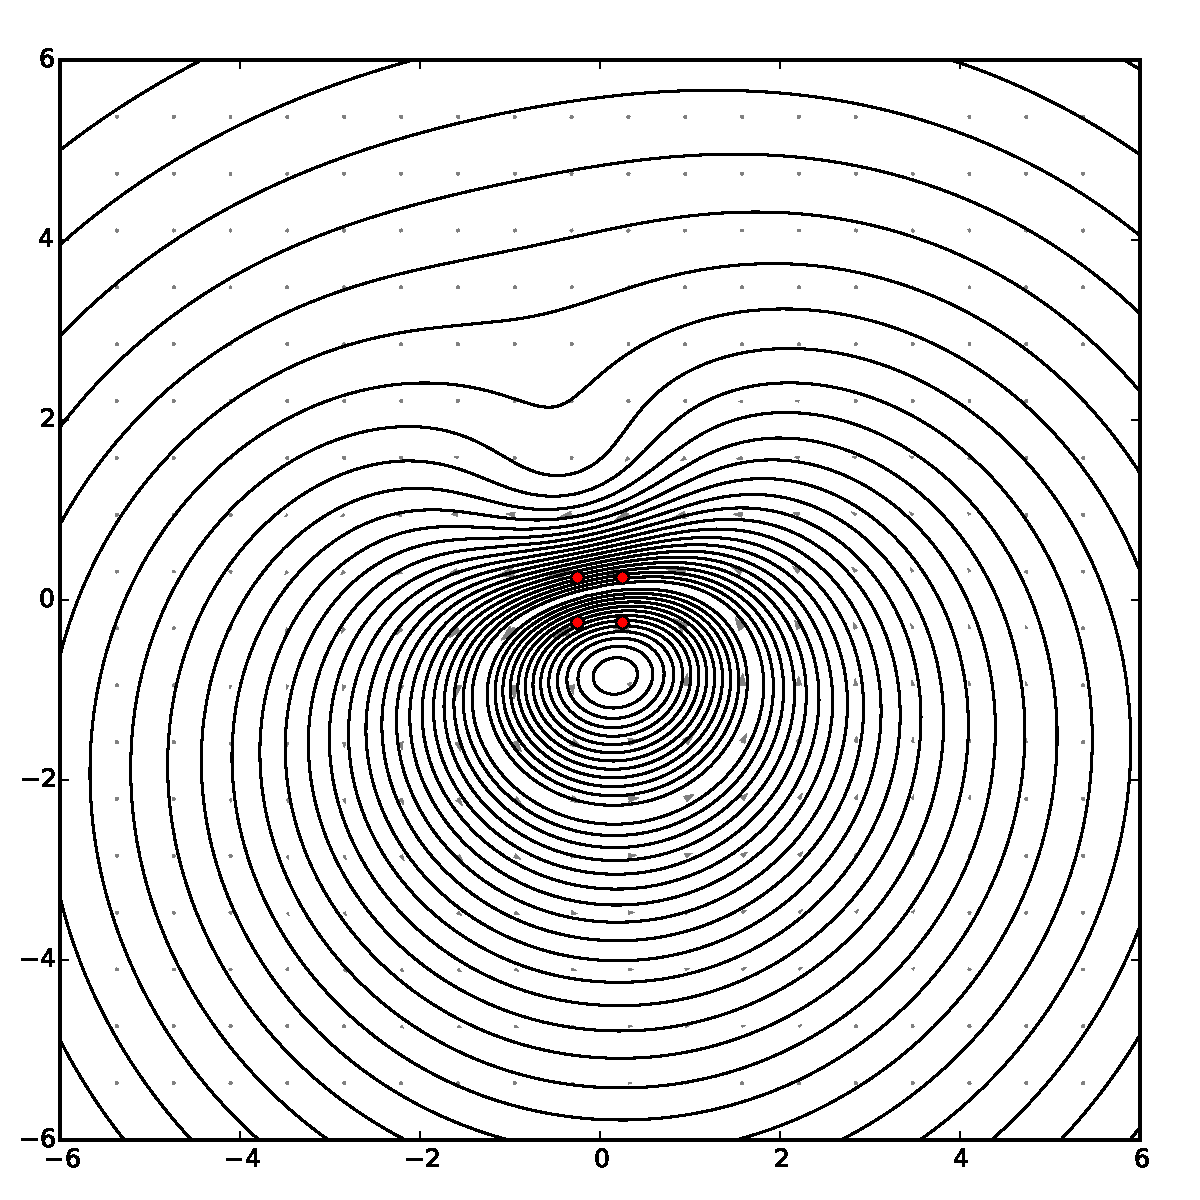
\includegraphics[width=0.15\textwidth]{./images/grouping_frames/order_0_time_0}
	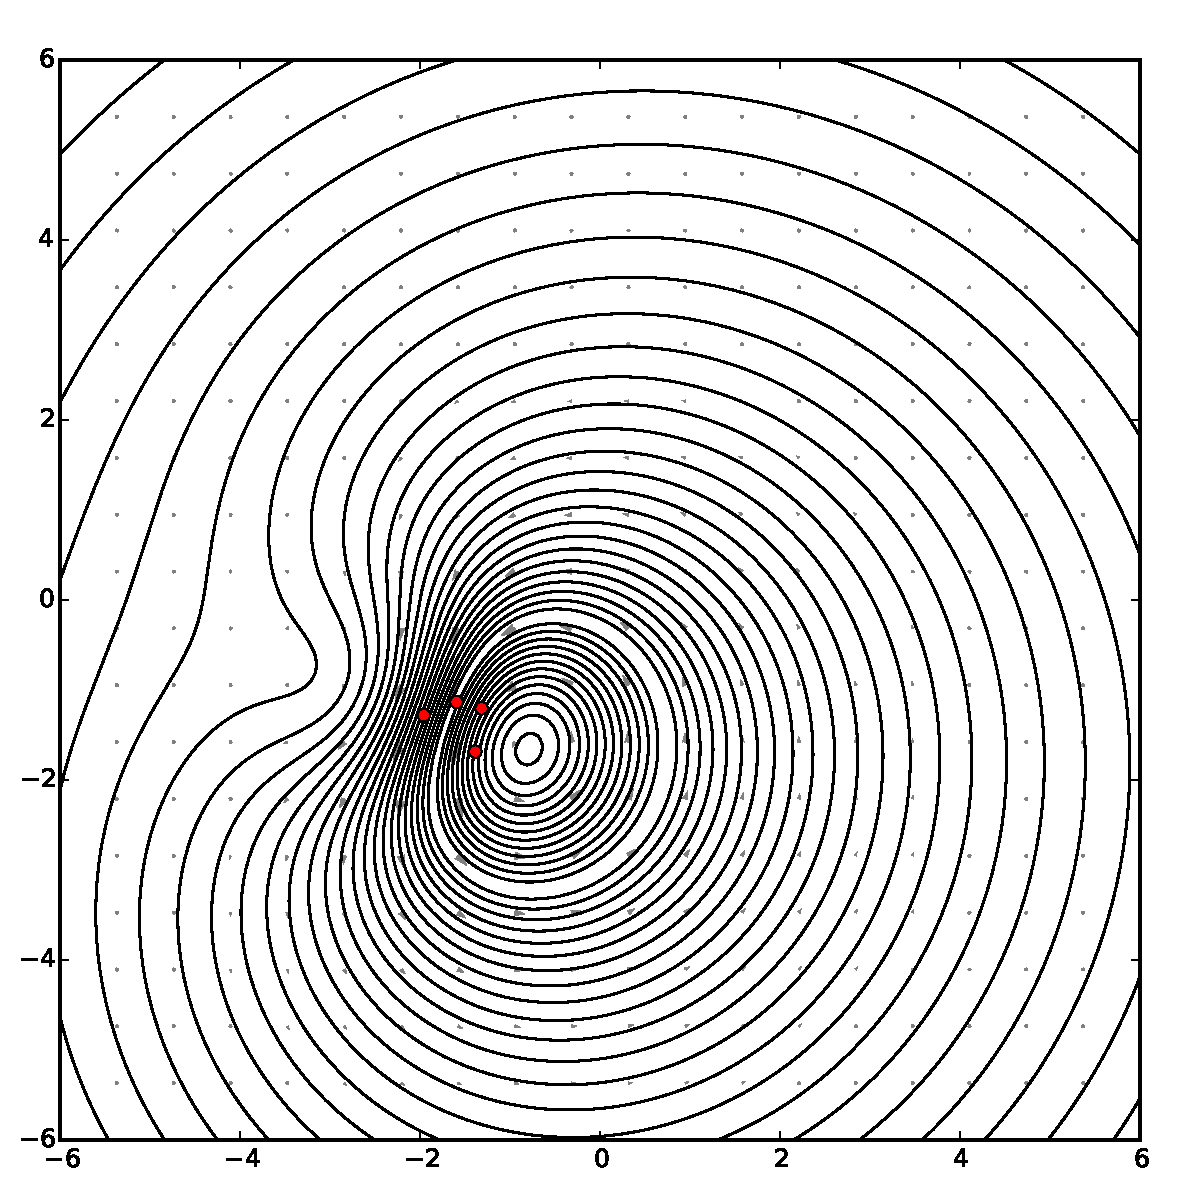
\includegraphics[width=0.15\textwidth]{./images/grouping_frames/order_0_time_51}
	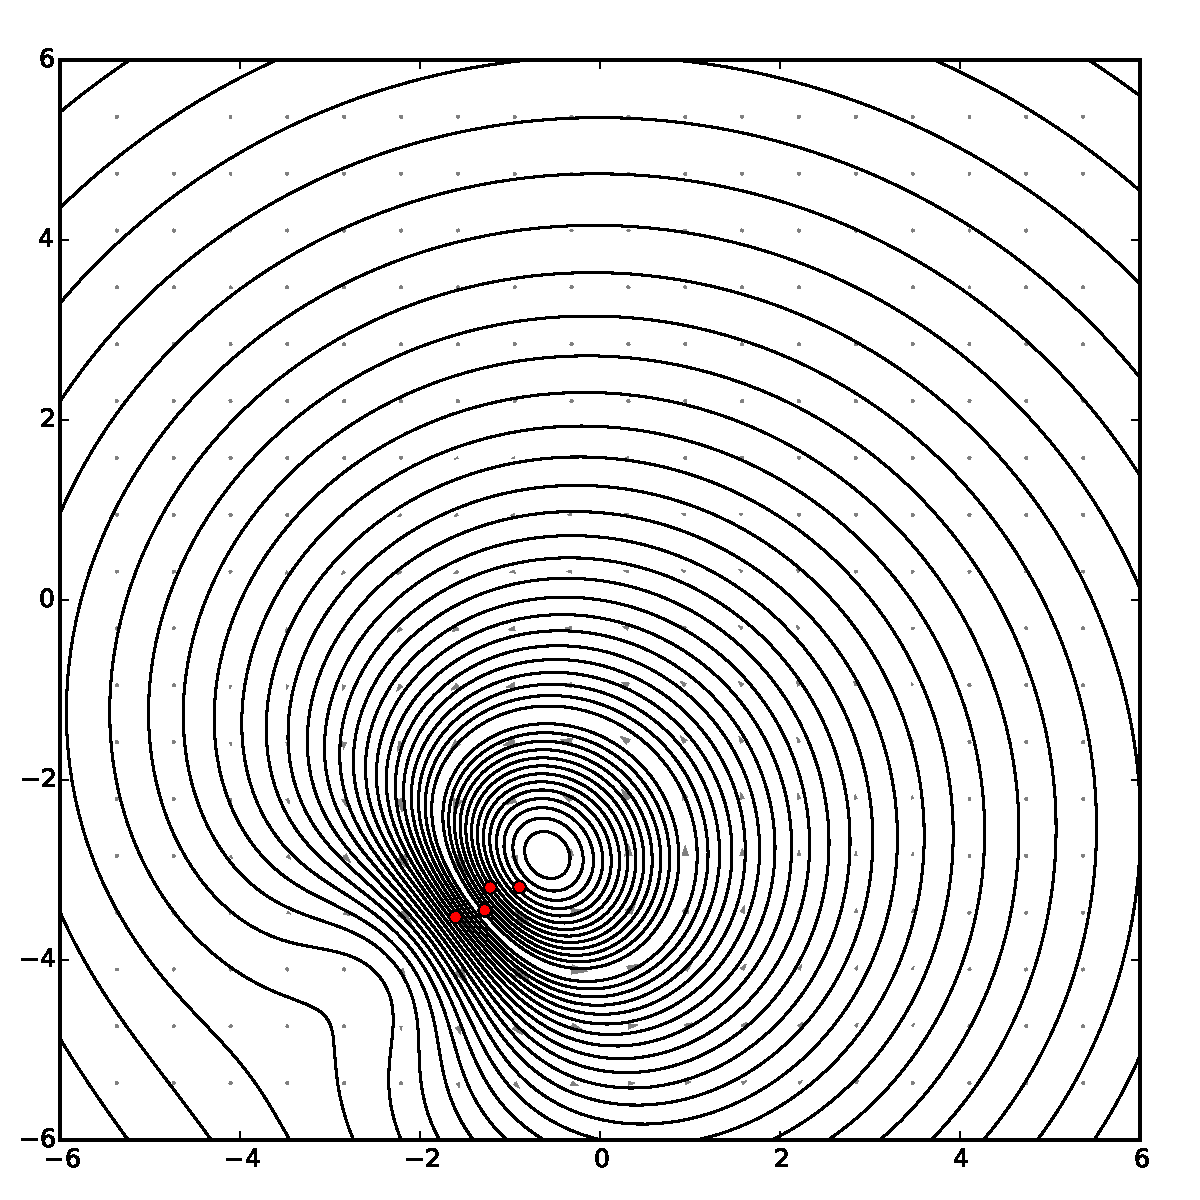
\includegraphics[width=0.15\textwidth]{./images/grouping_frames/order_0_time_101}
	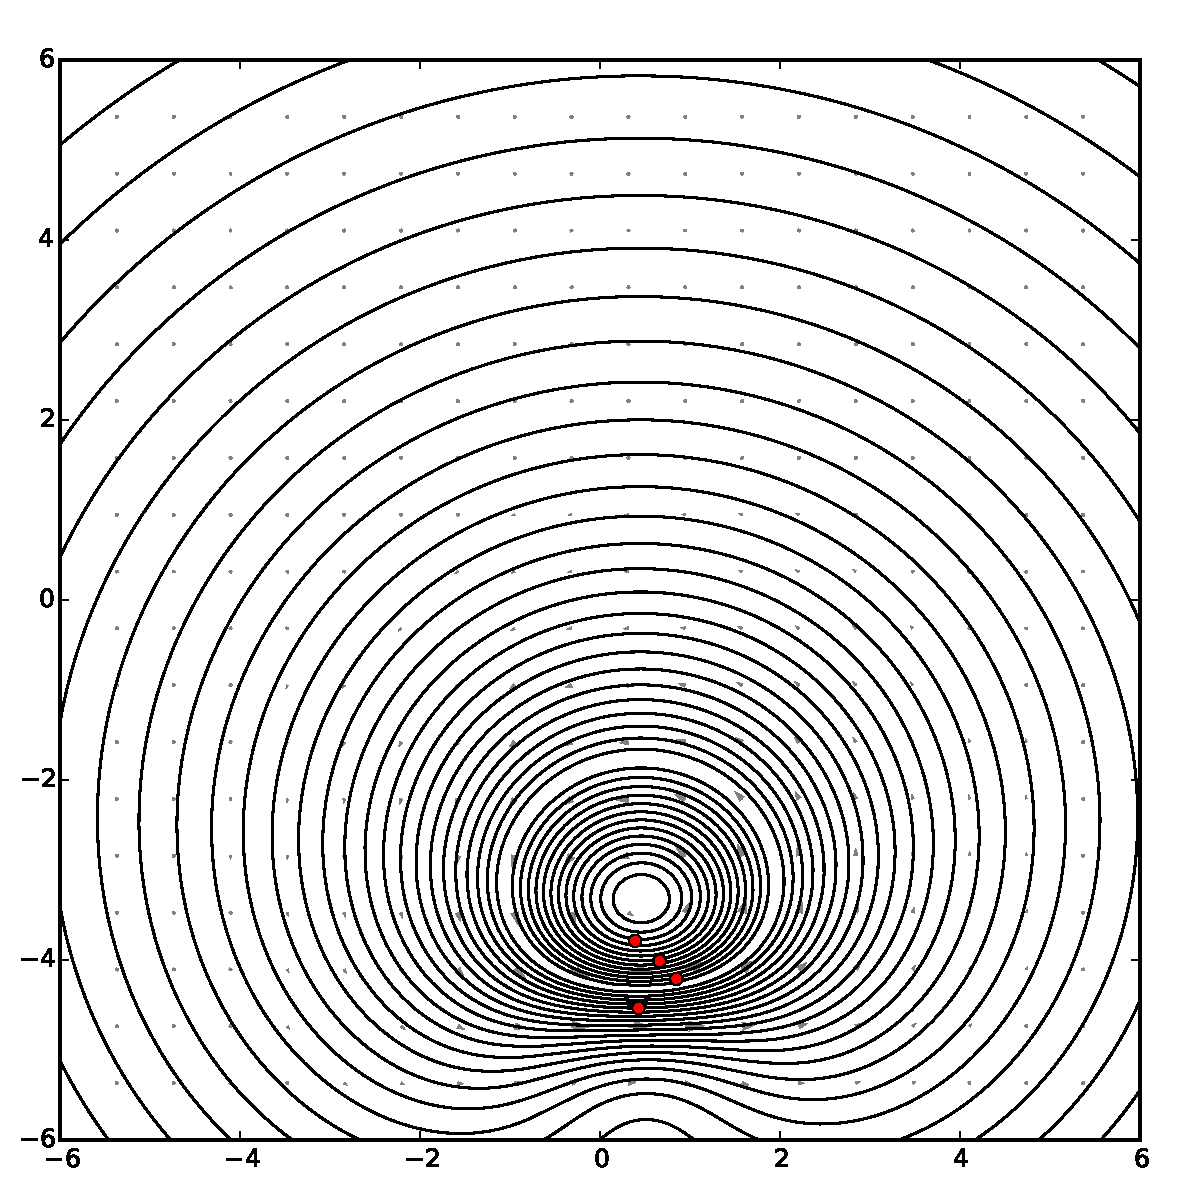
\includegraphics[width=0.15\textwidth]{./images/grouping_frames/order_0_time_152}
	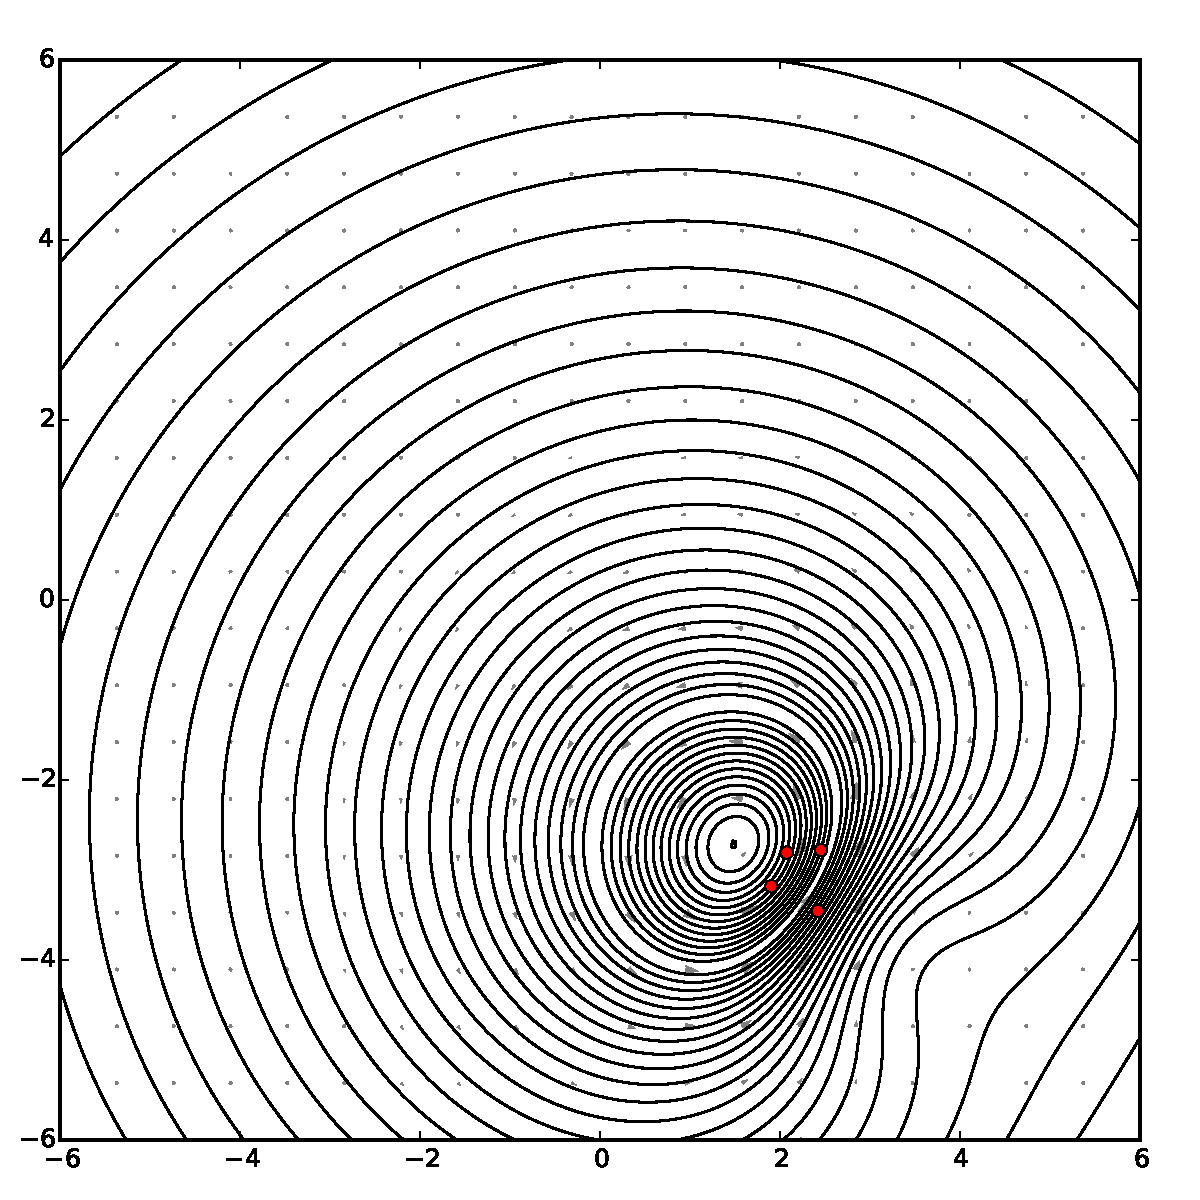
\includegraphics[width=0.15\textwidth]{./images/grouping_frames/order_0_time_202}
	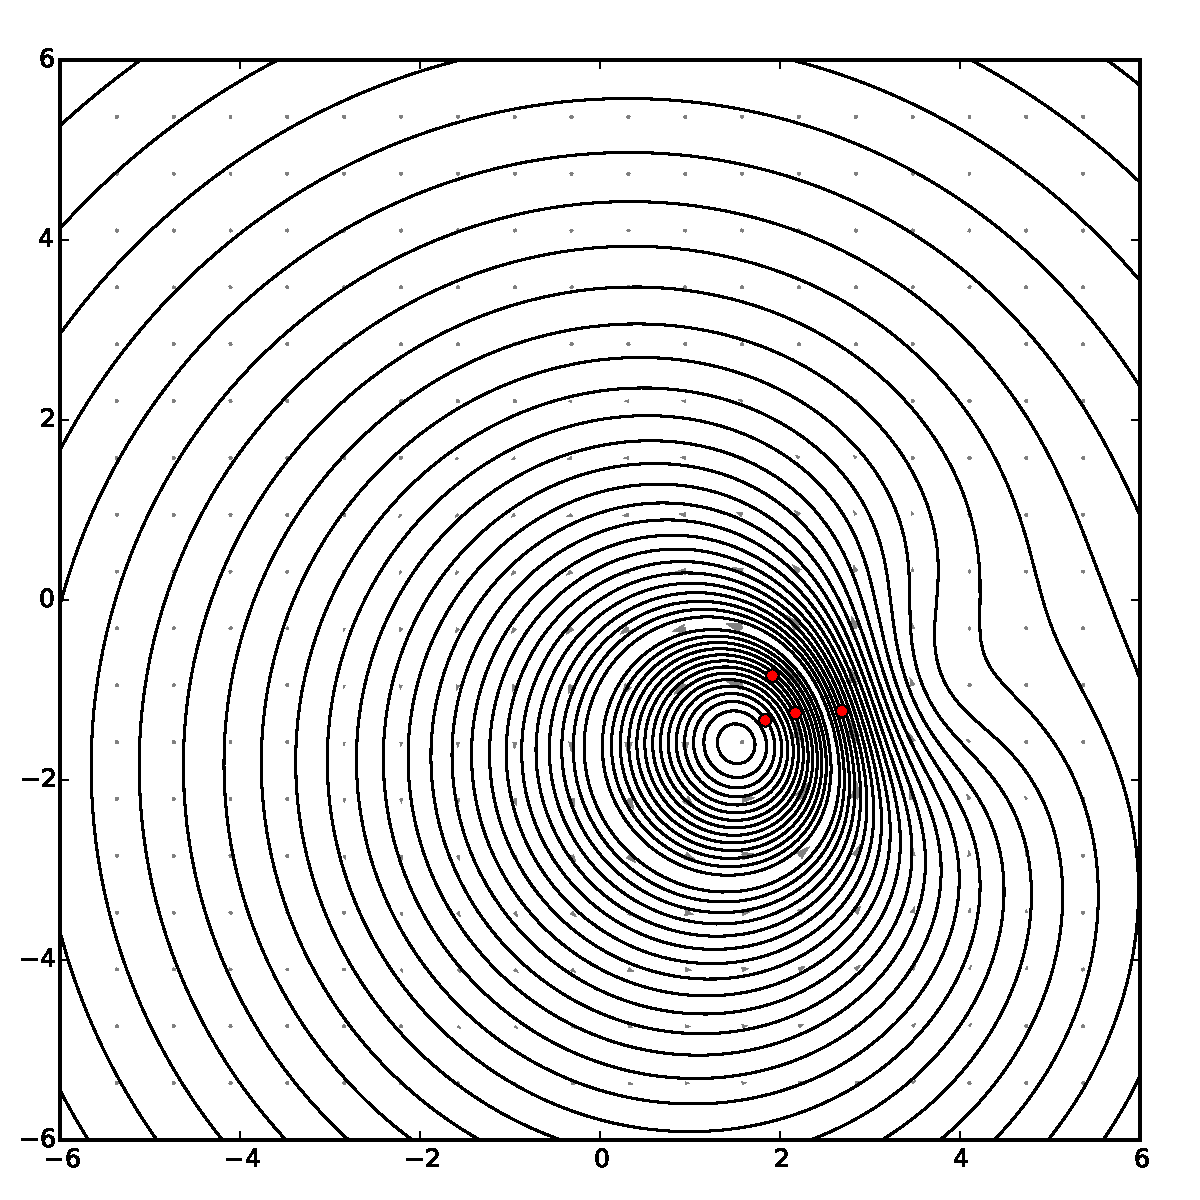
\includegraphics[width=0.15\textwidth]{./images/grouping_frames/order_0_time_253}	
	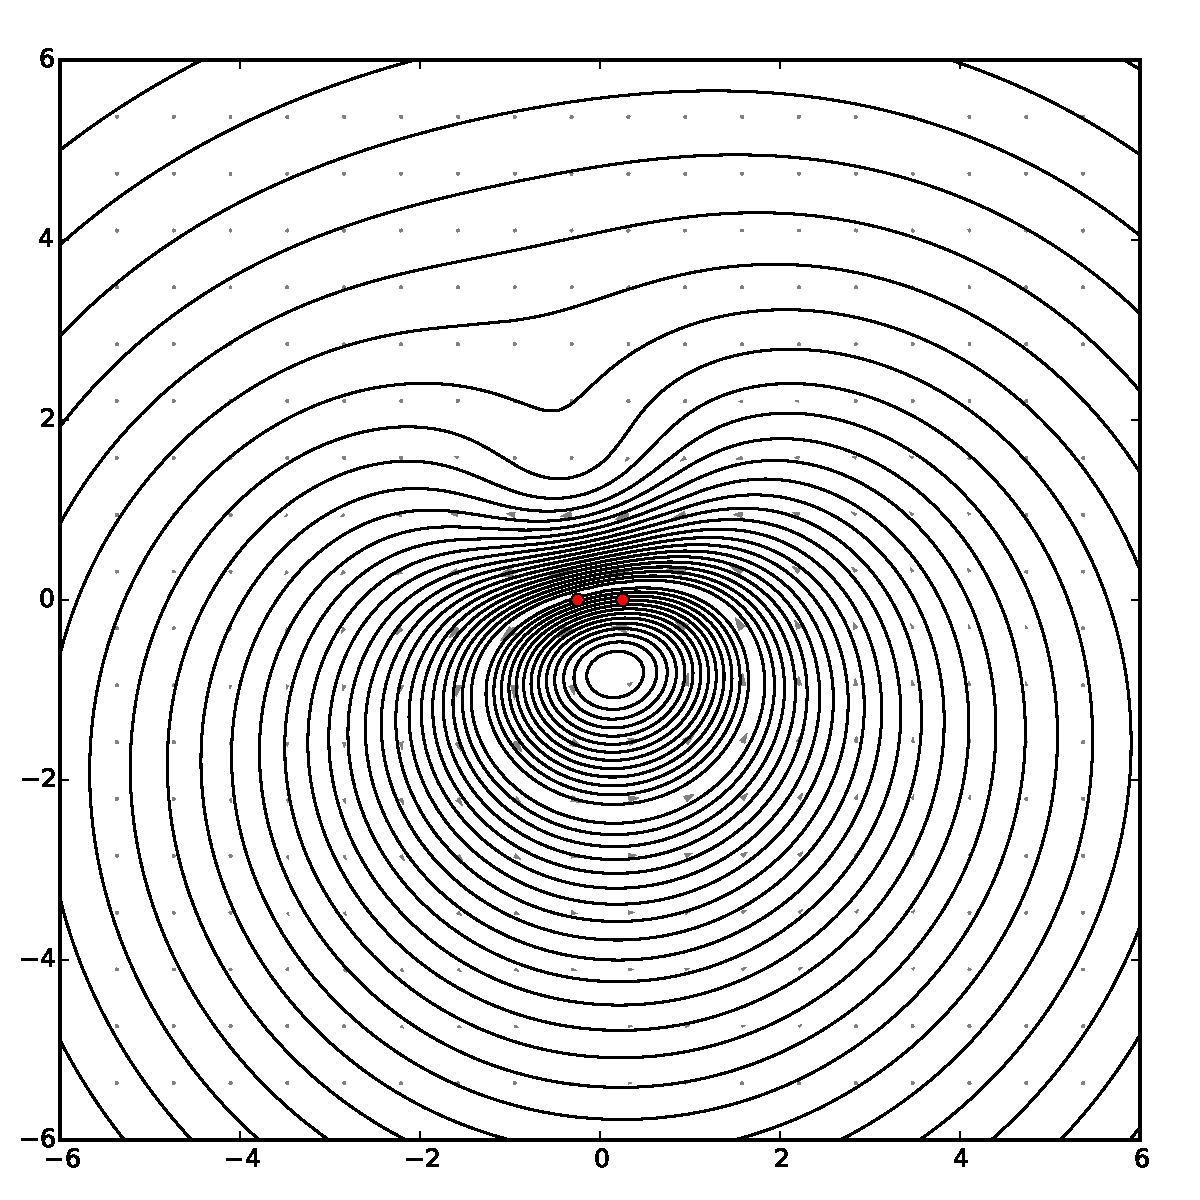
\includegraphics[width=0.15\textwidth]{./images/grouping_frames/order_1_time_0}
	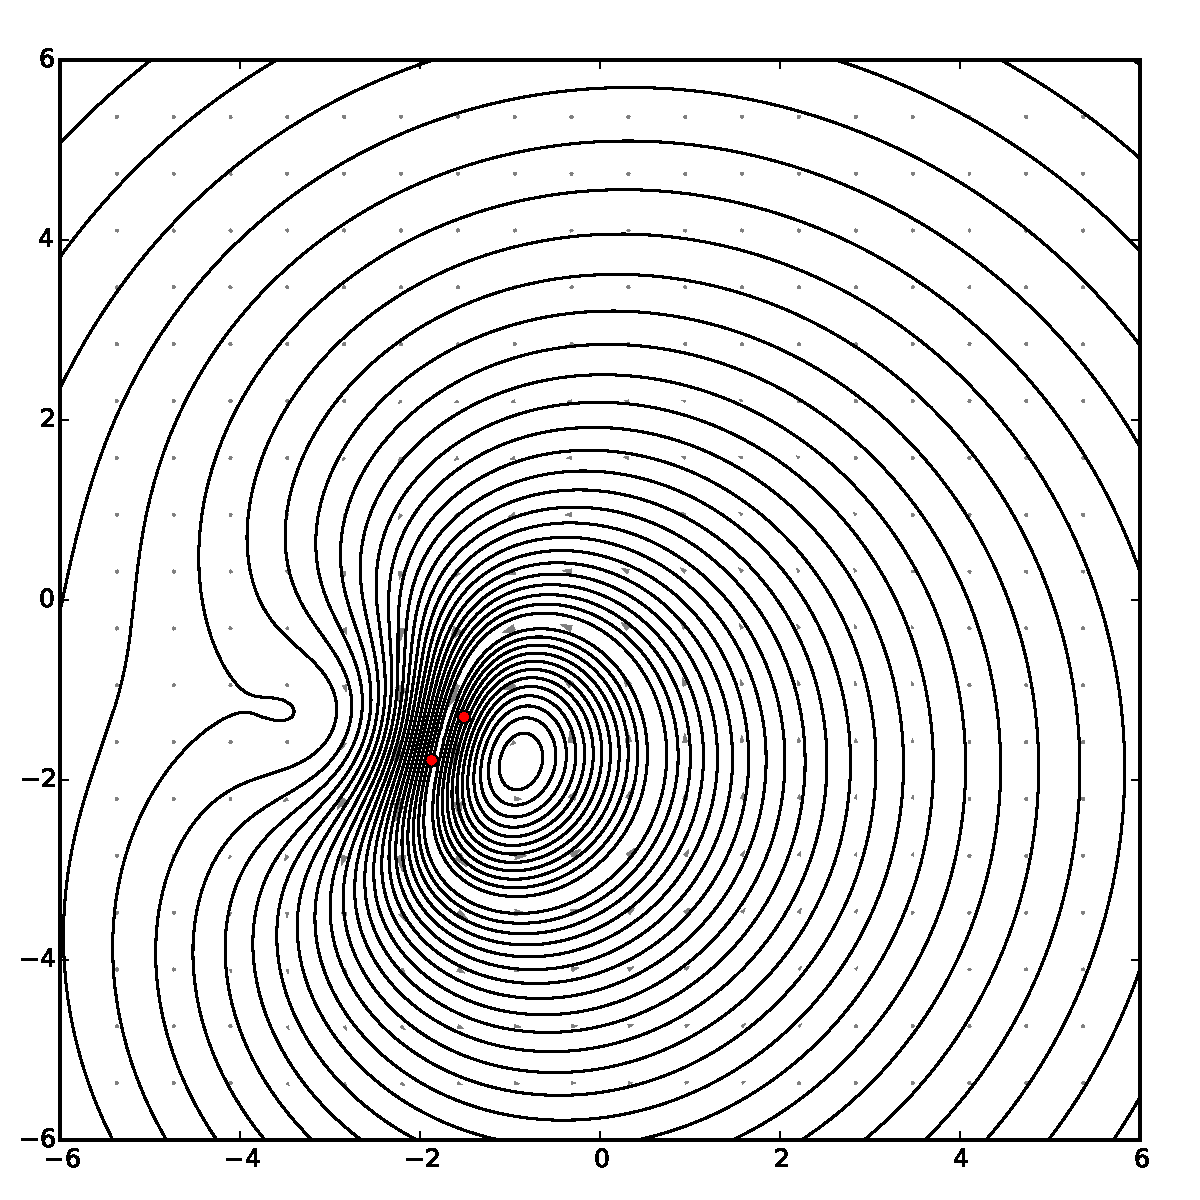
\includegraphics[width=0.15\textwidth]{./images/grouping_frames/order_1_time_51}
	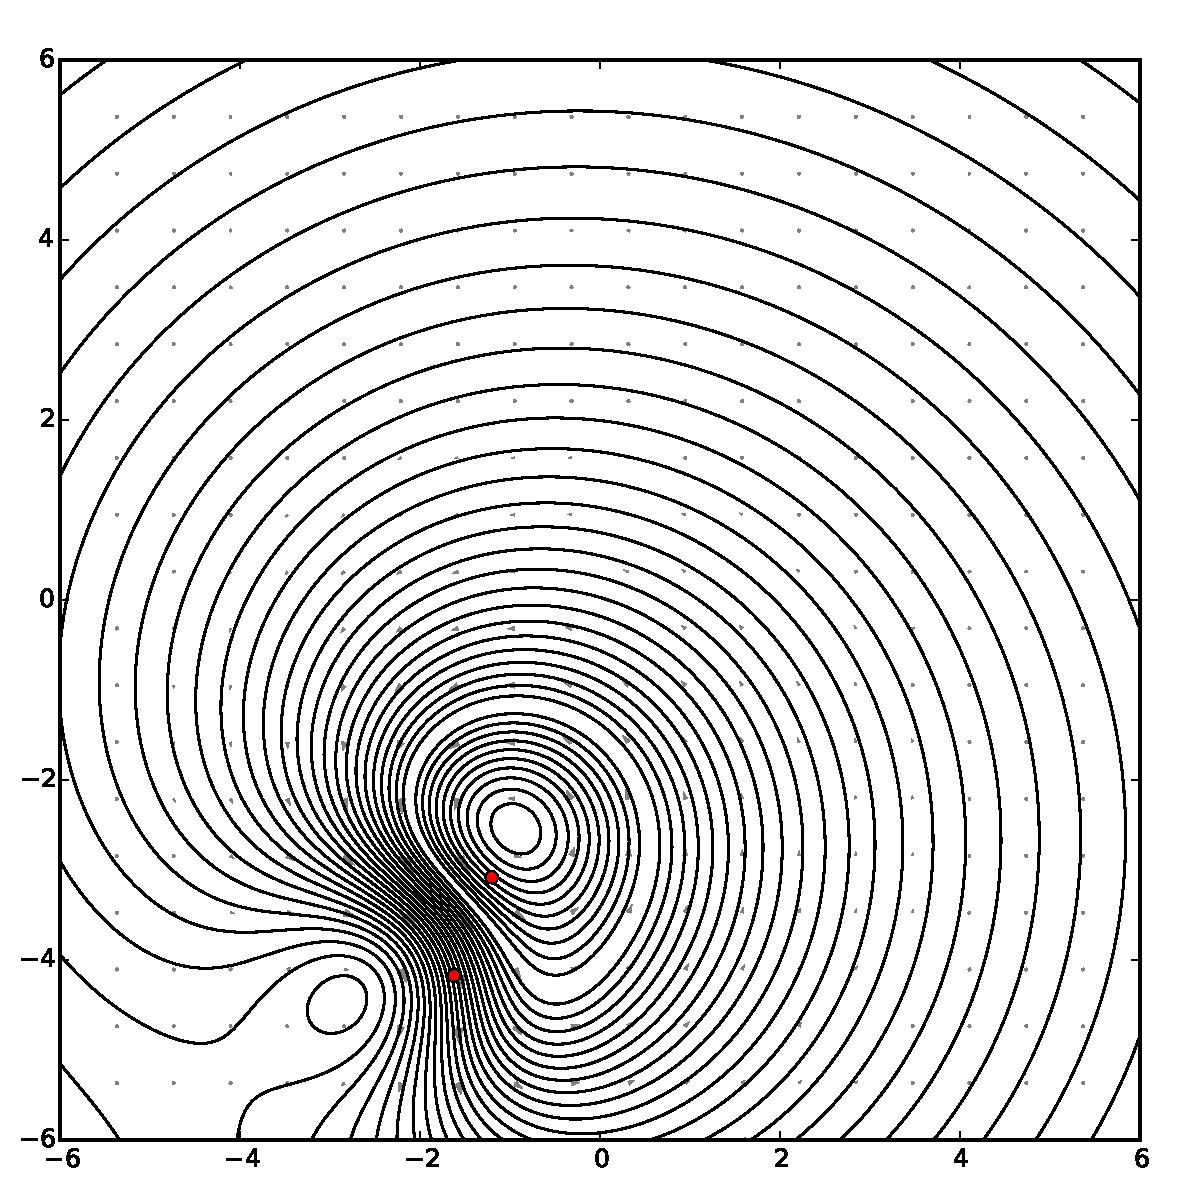
\includegraphics[width=0.15\textwidth]{./images/grouping_frames/order_1_time_101}
	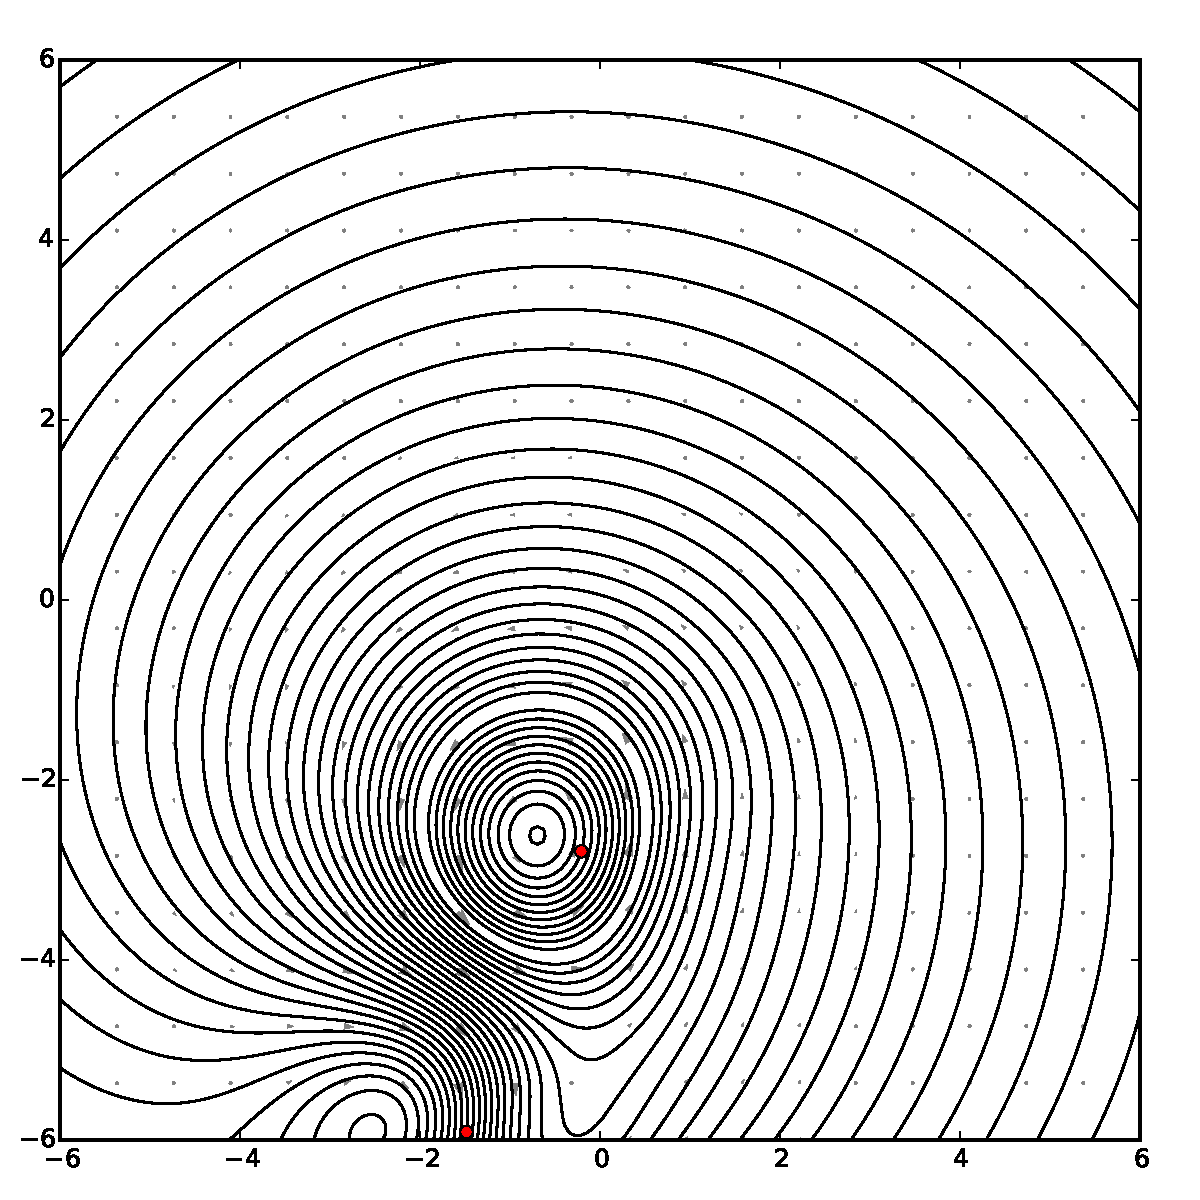
\includegraphics[width=0.15\textwidth]{./images/grouping_frames/order_1_time_152}
	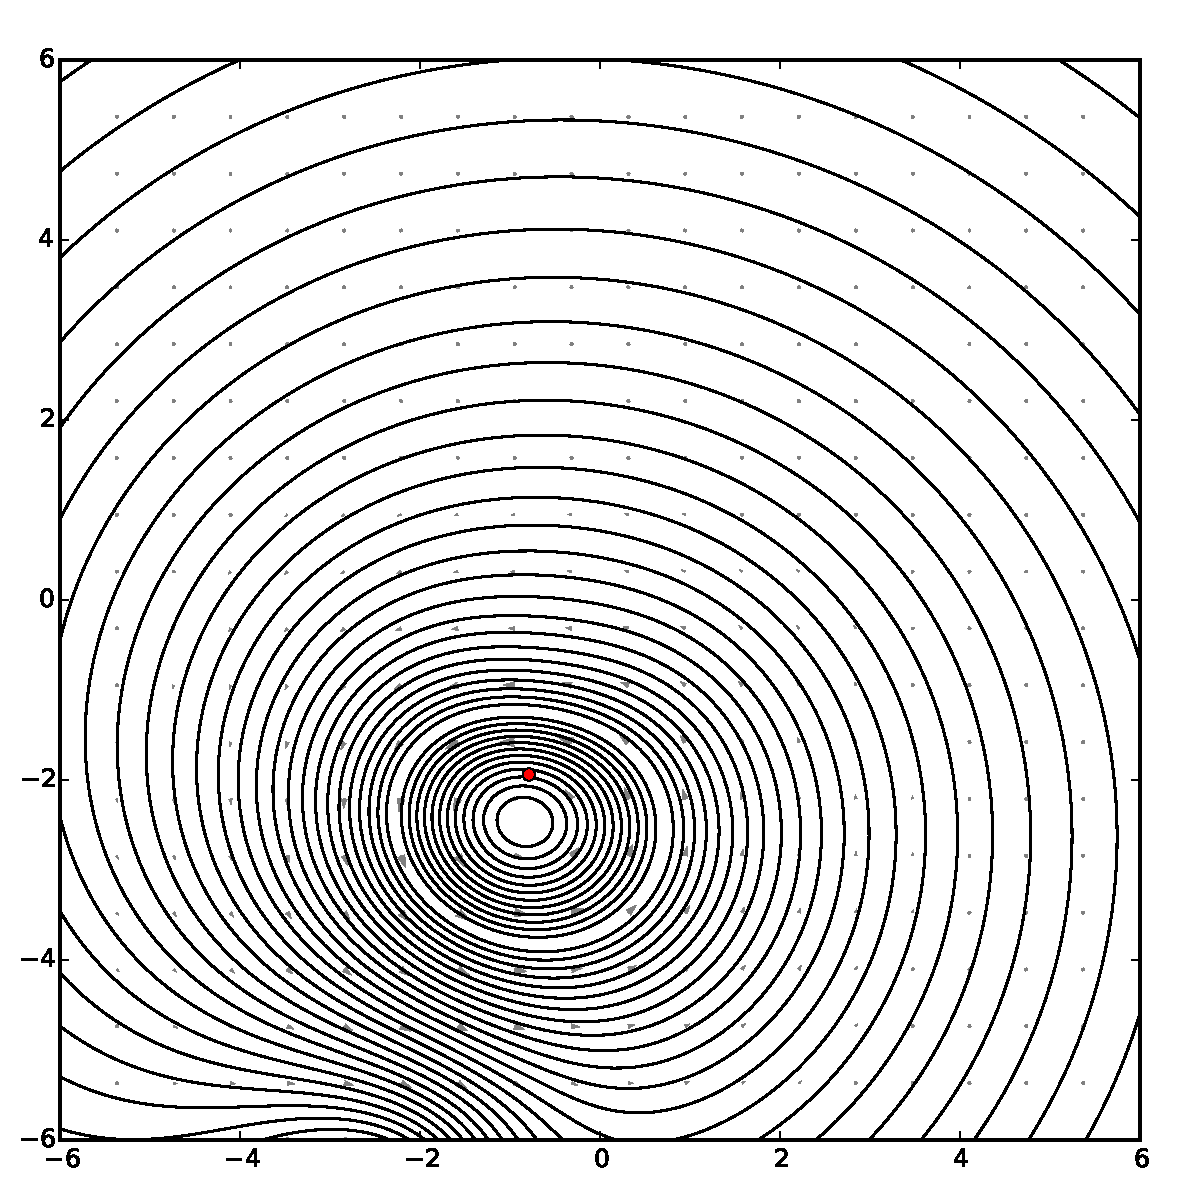
\includegraphics[width=0.15\textwidth]{./images/grouping_frames/order_1_time_202}
	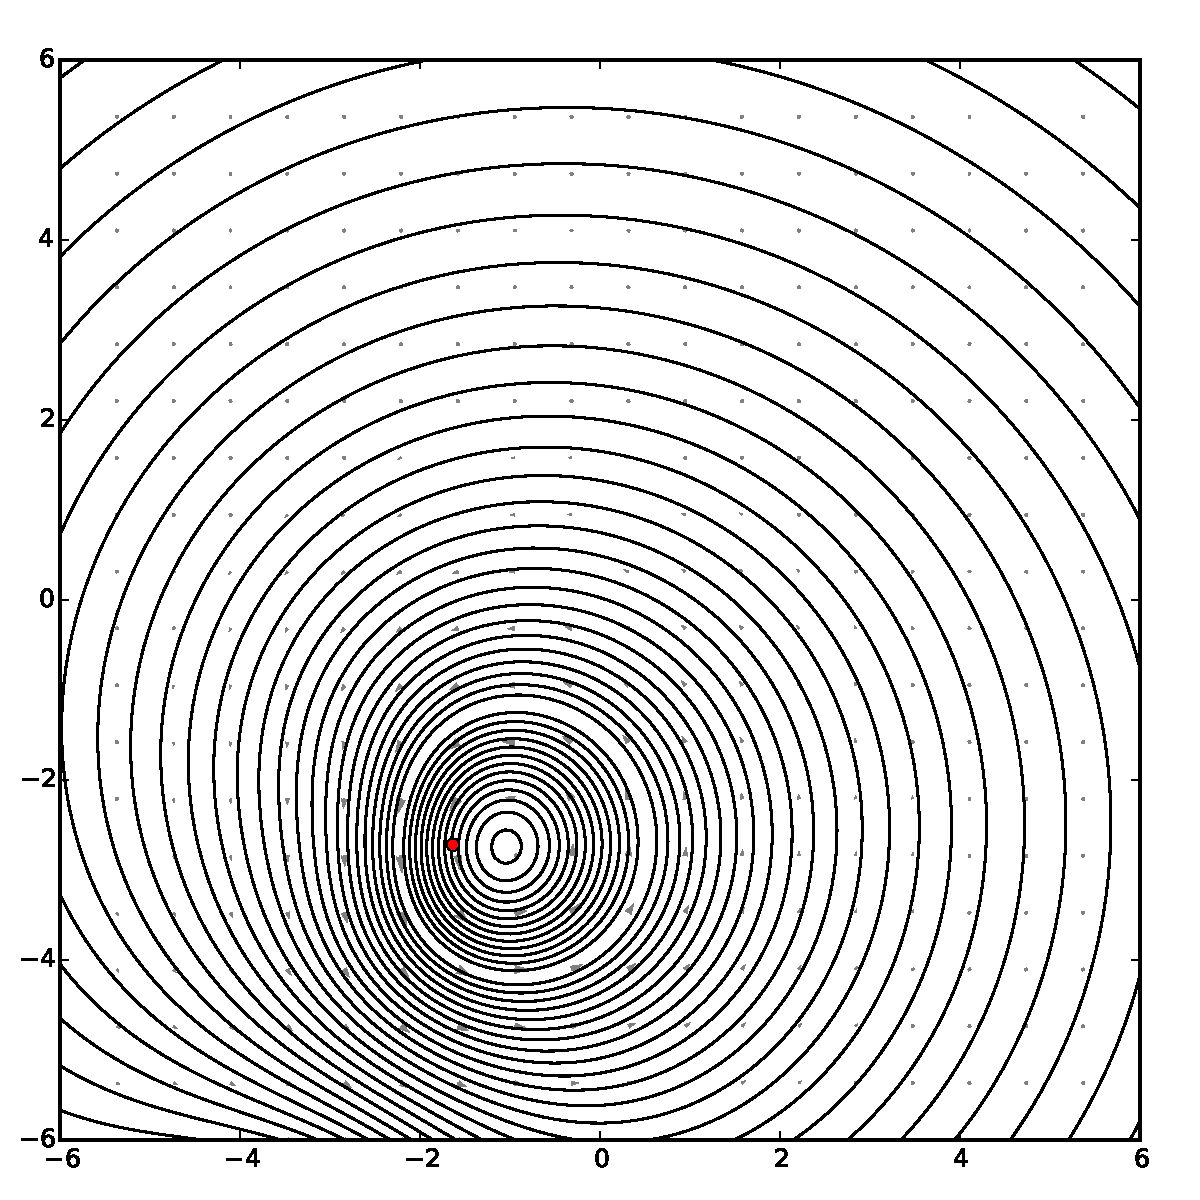
\includegraphics[width=0.15\textwidth]{./images/grouping_frames/order_1_time_253}	
	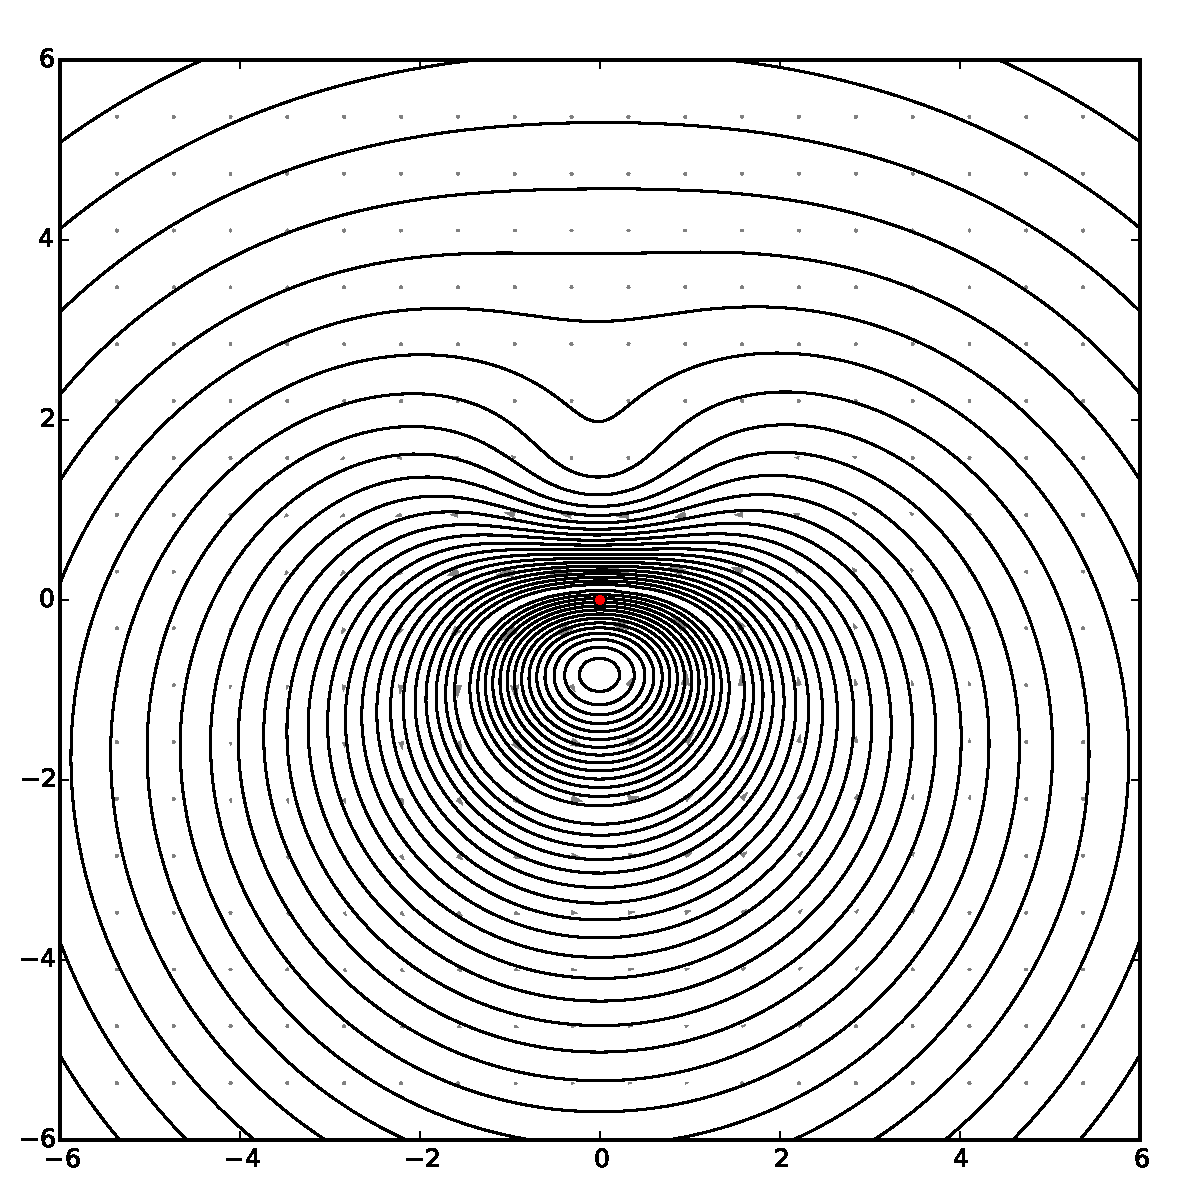
\includegraphics[width=0.15\textwidth]{./images/grouping_frames/order_2_time_0}
	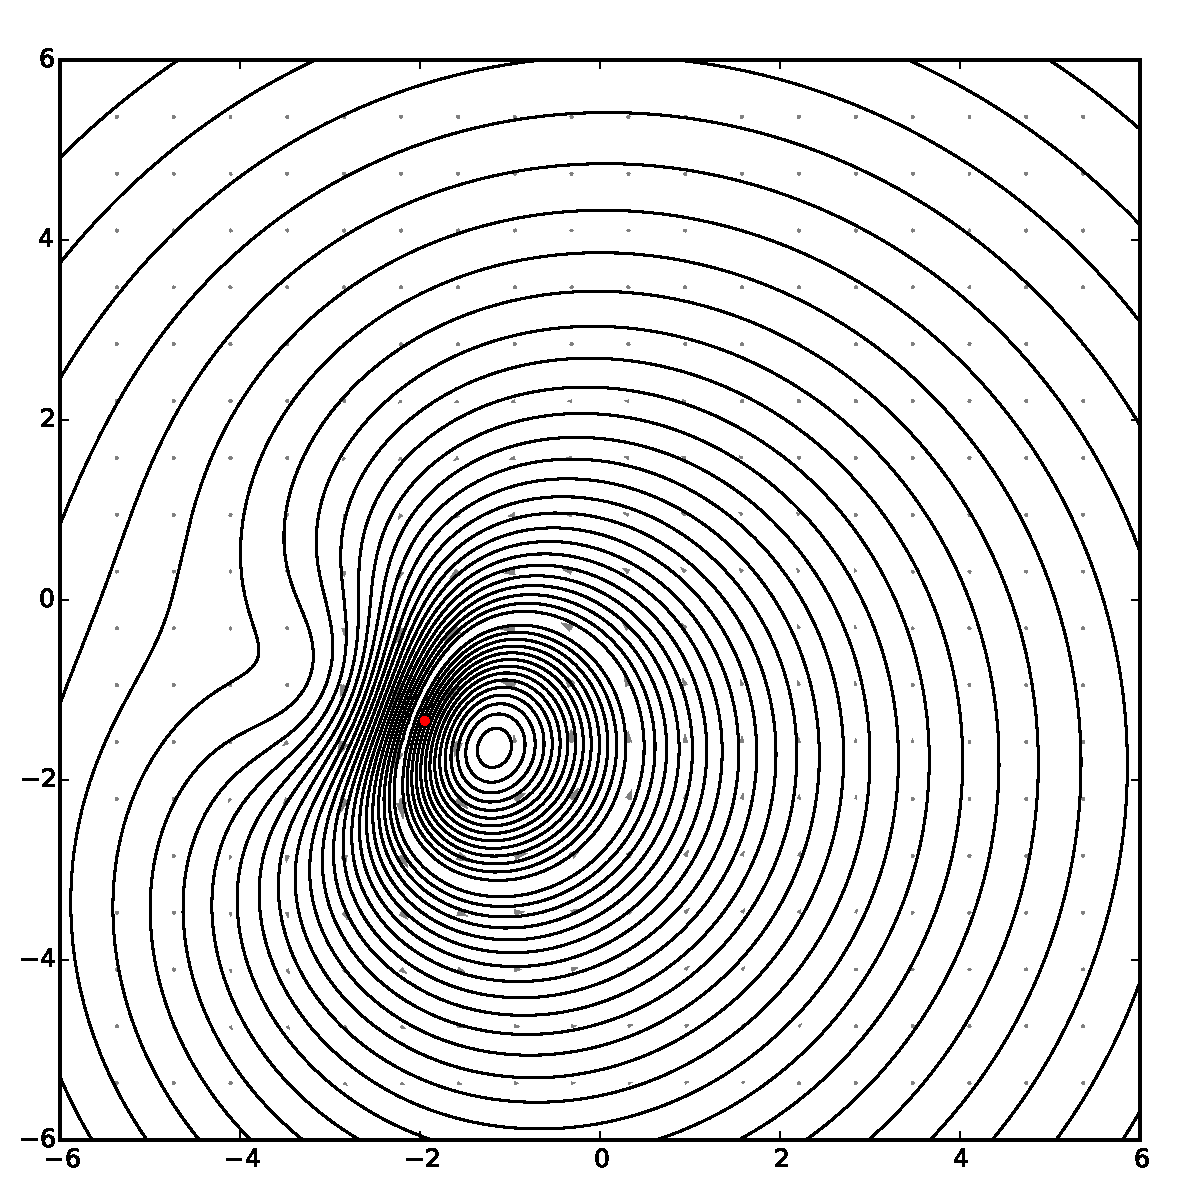
\includegraphics[width=0.15\textwidth]{./images/grouping_frames/order_2_time_51}
	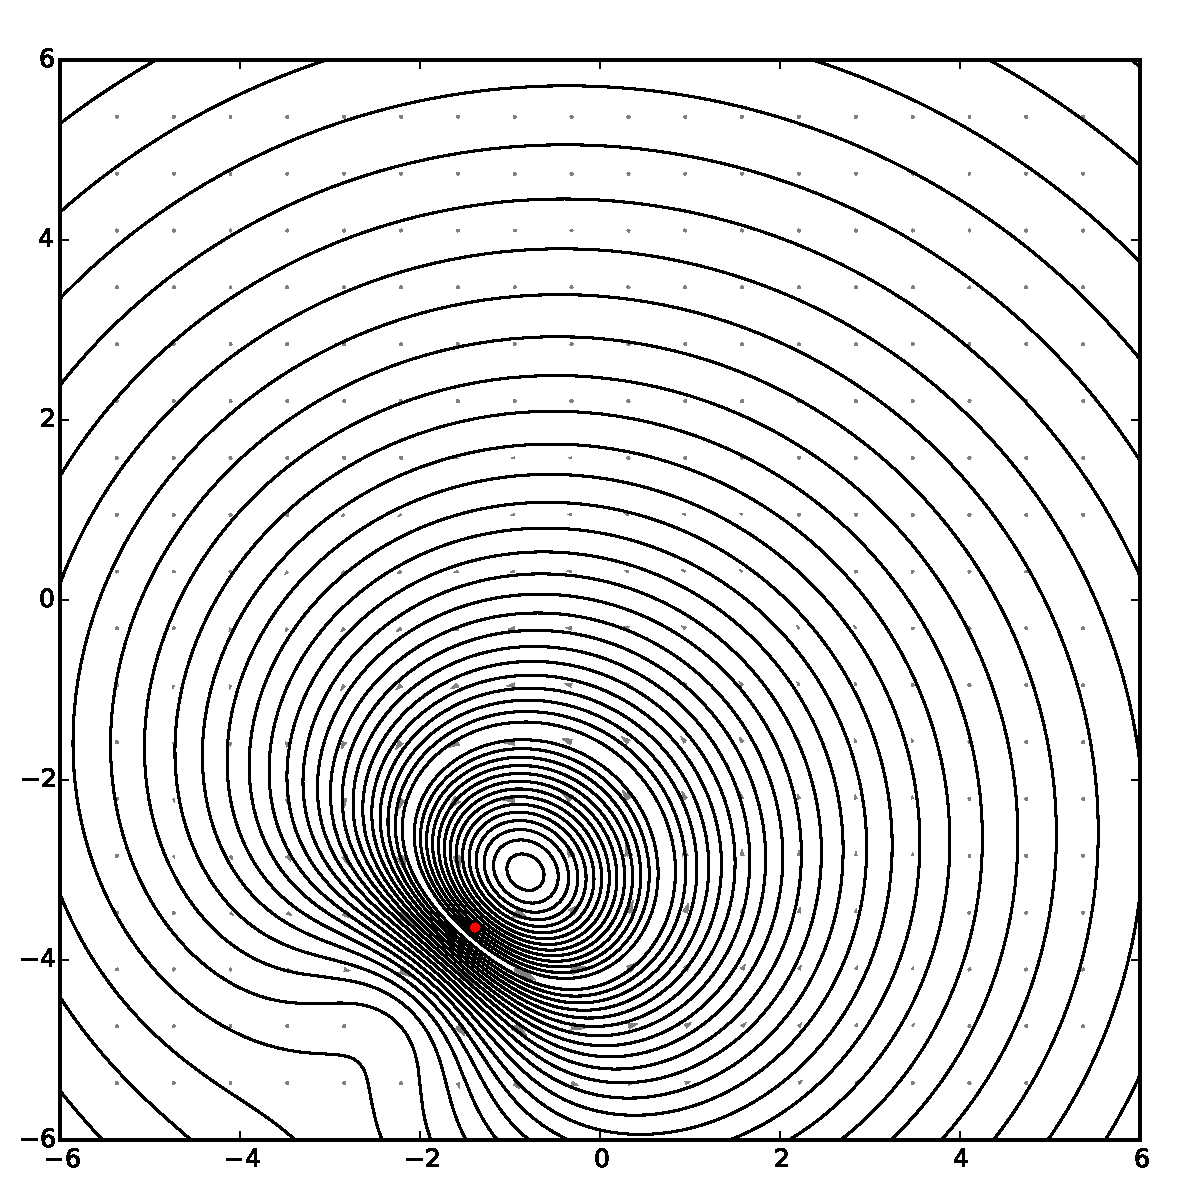
\includegraphics[width=0.15\textwidth]{./images/grouping_frames/order_2_time_101}
	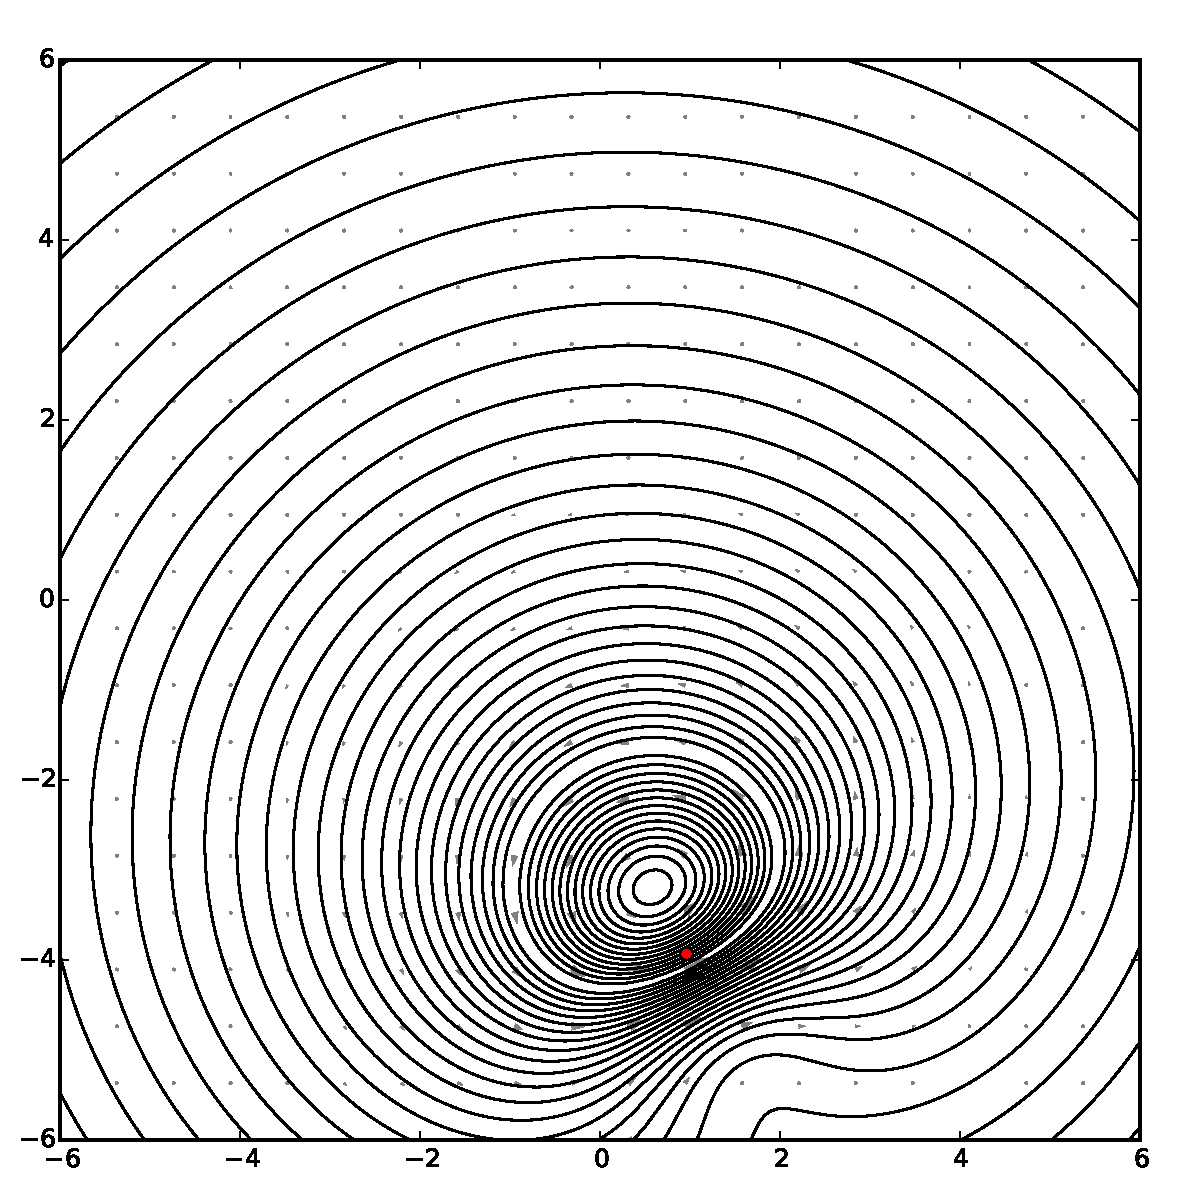
\includegraphics[width=0.15\textwidth]{./images/grouping_frames/order_2_time_152}
	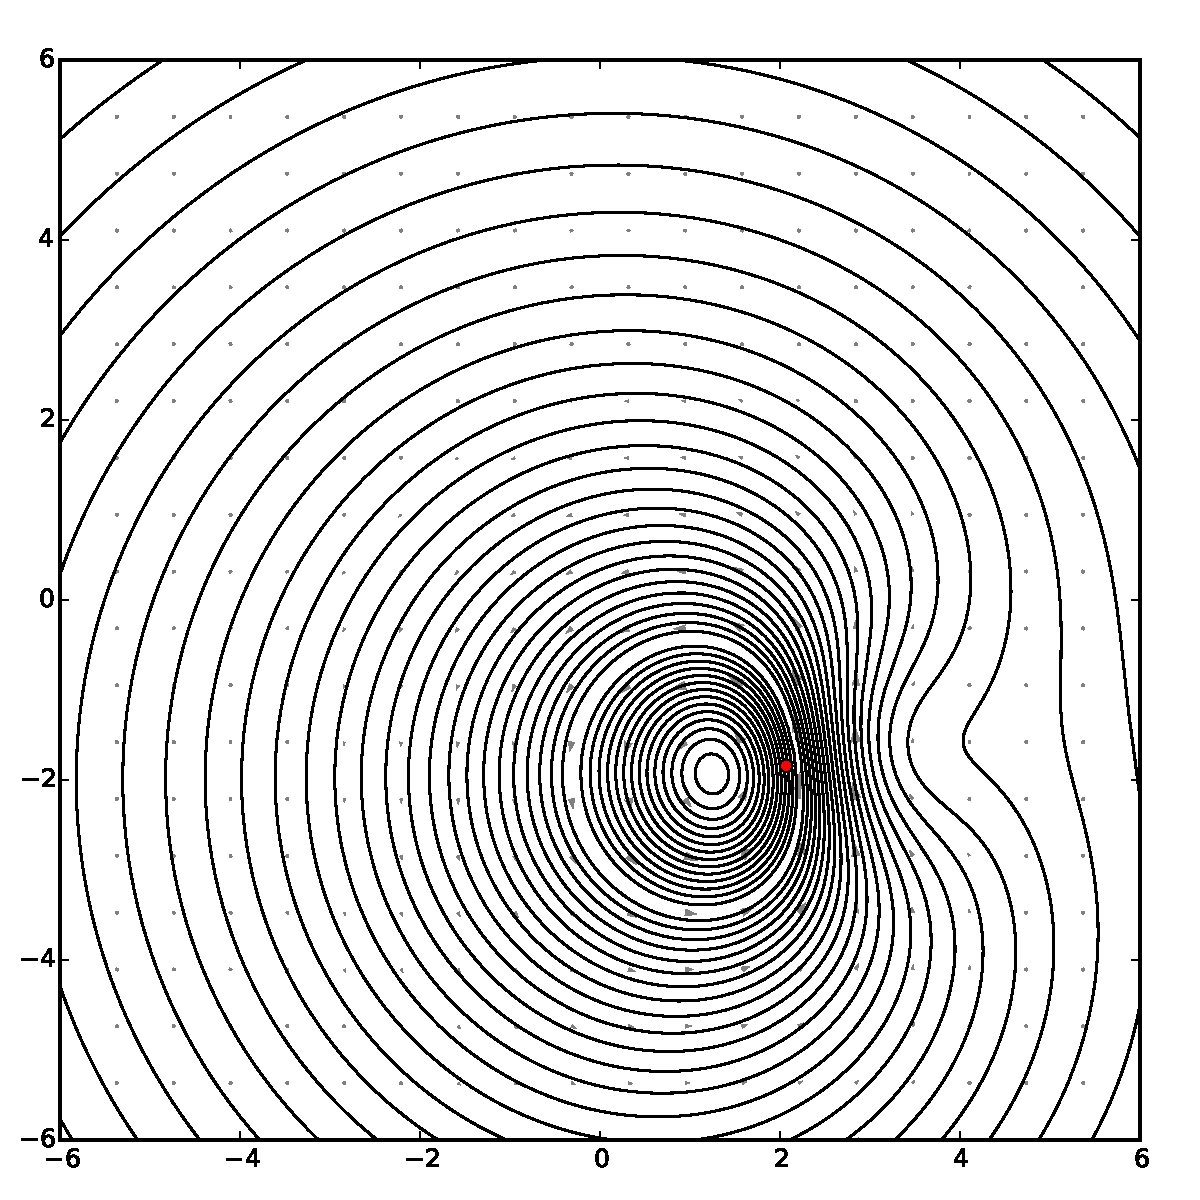
\includegraphics[width=0.15\textwidth]{./images/grouping_frames/order_2_time_202}
	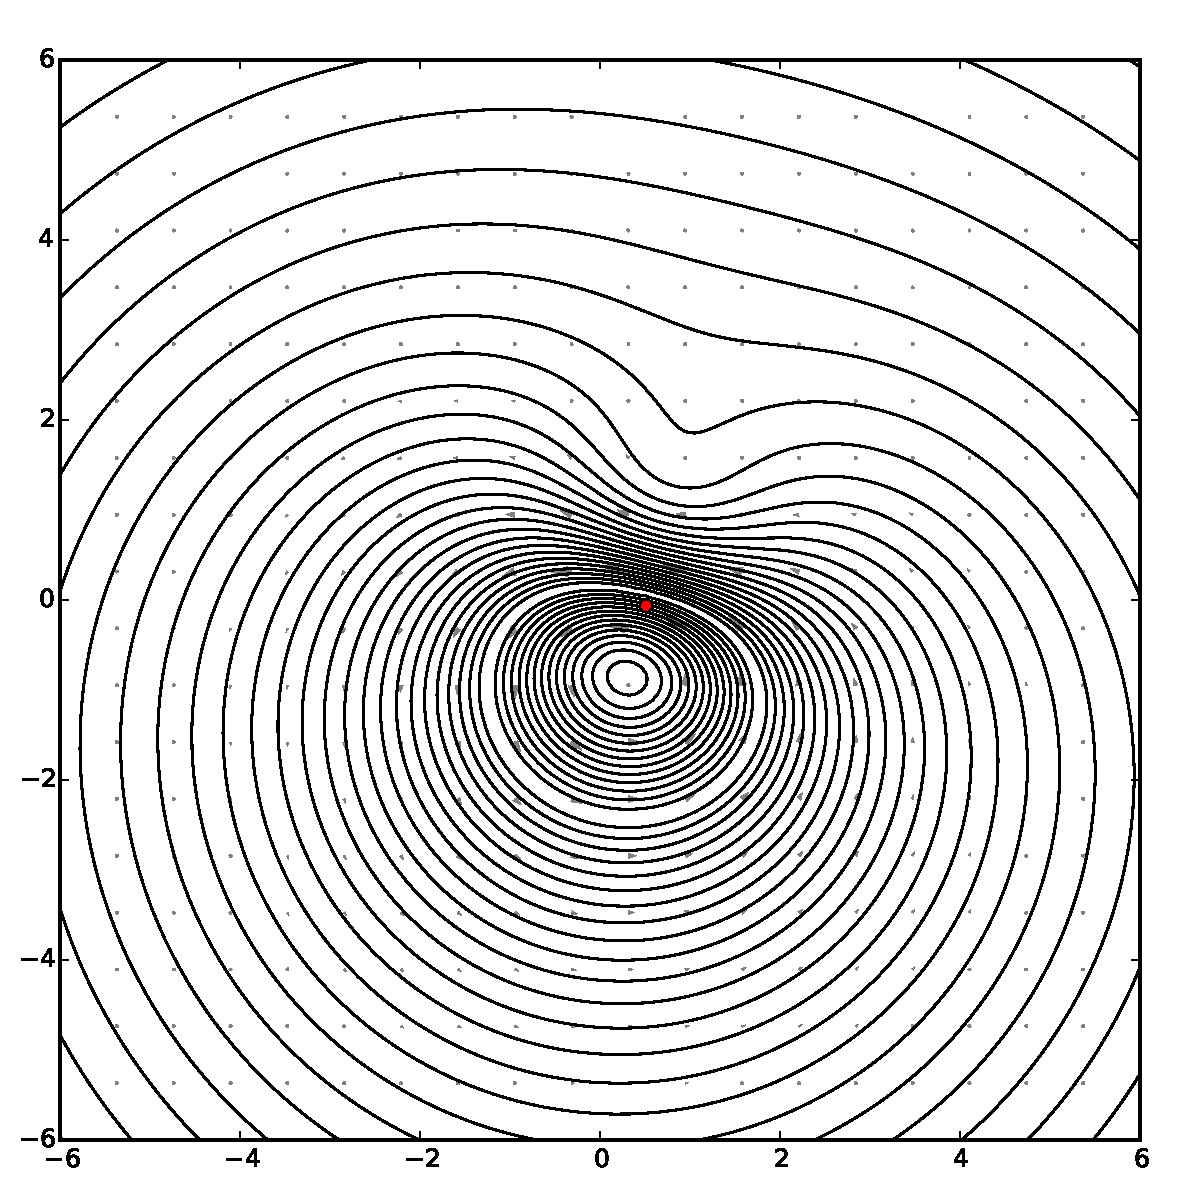
\includegraphics[width=0.15\textwidth]{./images/grouping_frames/order_2_time_253}
	\caption{Snapshots of the evolution for various initial conditions at time $t=0,51,101,152,202,253$.
		The top row depicts the evolution of four 0th order jet vortices given by the initial condition \eqref{eq:ic_0}.
		}
	\label{fig:grouping}
\end{figure}


\subsection{Approximation of initial conditions}
\label{sec:approximation}
In this section we will illustrate how the use of jet vortices can increase the accuracy of approximation of a vorticity field in a distributional sense.
We can begin by defining an inner-product on the space of distributions on $\R^2$, given by
\[
	\langle \omega_1 , \omega_2 \rangle_{G_\delta} := \int \omega_1(z) G_\delta (z - \tilde{z}) \omega_2(\tilde{z}) dz d\tilde{z}.
\]
Consequently, the energy of the fluid is given by $H(\omega) = \frac{1}{2} \|\omega\|^2_{G_\delta} = \frac{1}{2} \langle \omega,\omega\rangle_{G_\delta}$.

Let $0 < h \ll 1$ be small and define $h \mathbb{Z}^2 = \{ (ah,bh) \in \R^2 \mid (a,b) \in \mathbb{Z}^2 \}$.
Given an $\omega \in \mathcal{D}'(\R^2)$, we can attempt to approximate $\omega$ via Dirac-deltas supported on $h \mathbb{Z}^2$.
There is a natural way to do this with respect to the inner product $\langle \cdot , \cdot \rangle_{G_\delta}$.
We could define $\omega_h^{(0)} = \sum_{i \in \mathbb{Z}^2} \Gamma_i \delta_{z_i}$ by requiring the error, $\omega_h^{(0)} - \omega$, to be $\langle \cdot , \cdot \rangle_{G_\delta}$-orthogonal to $\delta_z$ for each $z \in h \mathbb{Z}^2$.
This means that $G_\delta *\omega(z) =  \sum_i \Gamma_i G_\delta (z-z_i)$ for each $z \in h\mathbb{Z}^2$.
Thus $\psi_h^{(0)} = \sum_i \Gamma_i G_\delta (z-z_i)$ can be seen as a $0$th order approximation to $\psi = G_\delta *\omega$
because $\psi_h^{(0)}(z) = \psi(z)$ for all $z \in h\mathbb{Z}$.
 
The same reasoning applies if we consider $\omega^{(k)}_h = \sum_{i,m+n \leq N} \Gamma_i^{mn} \partial_x^m \partial_y^n \delta_{z_i}$.
We define the scalars $\Gamma_i^{mn}$ via the equations
\begin{align*}
  \partial_x^\ell \partial_y^k \psi (z_i) = \sum_j (-1)^{m+n} \Gamma_j^{mn} \partial_x^{m+\ell} \partial_y^{n+k} G_\delta(z_i - z_j)
\end{align*}
for $\psi = G_\delta*\omega$, $z_i \in h \mathbb{Z}^2$, and $|\beta| \leq k$.
Then $\psi^{(k)}_h (z)= \sum_{i,\alpha} (-1)^{m+n} \Gamma_k^{mn} \partial_x^m \partial_y^n G_\delta( z - z_i)$
serves as an order $k$ approximation of $\psi$ when $\psi \in C^k$.

This is not to say that the convergence rate is simply $O(h^k)$.
The convergence of the initial condition, and in fact the full fluid system
upon integrating the equations of motion, is a spectral convergence.
Moreover, this spectral convergence rate of the full system relies heavily on the choice of kernel
\cite{BealeMajda1982}.

As an example, we numerically compute the corresponding approximations of the stream function
\begin{align}
        \psi(x,y) = \exp( - r^2 ) - \exp( - r^2 / 2 )
        \label{eq:psi_exact}
\end{align}
The results are depicted in Figure \ref{fig:convergence}.
As we are unable to grid all of $\mathbb{R}^2$, the error
is only measured on a small subregion ($-3<x<3, -3<y<3$) within the region covered by our grid
($-6<x<6, -6 < y < 6 $).
We observe the predicted spectral convergence using jet vortices at orders zero, one, and two.
In each case, a grid spacing is reached where the convergence proceeds no further (possibly 
due to machine precision).
Nonetheless, higher order jet vortices appear to out perform lower order ones for smaller grid spacings.
\begin{figure}[h]
        \centering
        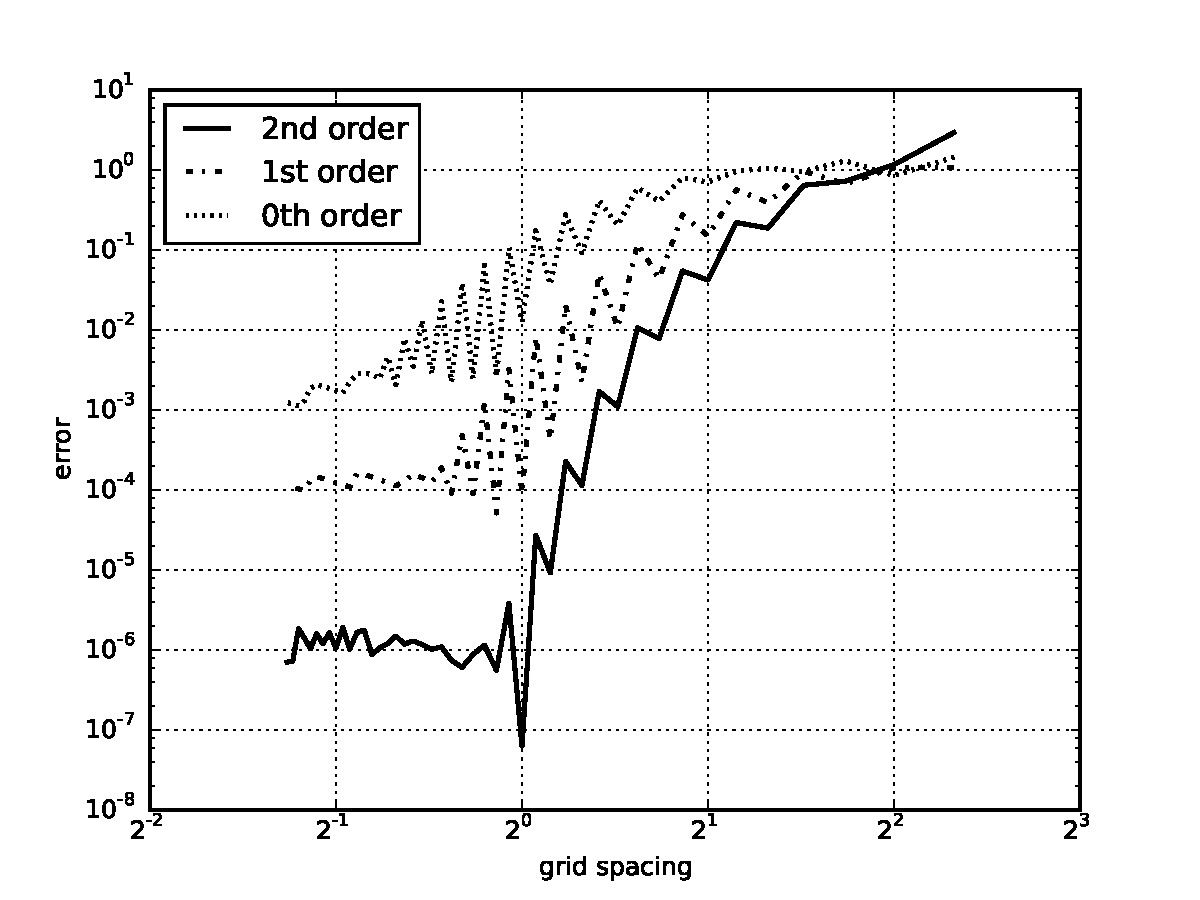
\includegraphics[width=0.7\textwidth]{./images/convergence.pdf}
        \caption{A convergence plot of the error in the sup-norm
        of the reconstructed stream function approximated using jet vortices of order $0$, $1$, and $2$.
        The method converges spectrally, so no specific convergence rate is observed.}
        \label{fig:convergence}
\end{figure}

\section{Numerical experiments}
\label{sec:numerical_experiments}
In these section we present the results of numerical experiments involving small numbers of vortices, for $N=1,2$, and $3$.

\subsection{Behavior of isolated jet vortices}
\label{sec:singles}
Next, we will briefly explore the behavior of a single isolated $k$th order jet vortex with $\Gamma^{mn} = 0$ with $m+n < k$ for $k=0,1,2$.
This case allows us to investigate the dynamics induced by the higher order circulation variables
in the absence of the lower order ones.

\subsection{Order 0}
The behavior of a single $0$th order jet vortex is explicitly solvable because the dynamics is stationary.

\subsection{Order 1}  
The behavior of a single $1$st order jet vortex with $\Gamma= 0$ is explicitly solvable.
Given the initial condition $(x(0) , y(0) ,  \Gamma (0) , \Gamma^x(0) , \Gamma^y(0) )$ with $\Gamma(0) = 0$ we find
\begin{align*}
	&x(t) = x(0) + v^x \,,\quad \quad y(t) = y(0) + v^y \,,\quad \quad \Gamma(t) = \Gamma(0) \\
	&\Gamma^x(t) = \Gamma^x(0)\,,\quad \quad \Gamma^y(t) = \Gamma^y(0)
\end{align*}
where $v^x = \Gamma^x(0) \partial_{xy}G_\delta(0) + \Gamma^y(0) \partial_{yy}G_\delta(0)$
and $v_y =  -\Gamma^y(0) \partial_{xy}G_\delta(0) - \Gamma^x(0) \partial_{xx}G_\delta(0)$.
In Figure \ref{fig:singleton_order1}
we depict such a trajectory with initial condition
\begin{align}
	x(0) = -3 , y(0) = -3 , \Gamma(0) = 0 , \Gamma^x = 1, \Gamma^y = 1 \label{eq:ic_order1}
\end{align}

\begin{figure}[h!]
	\centering
	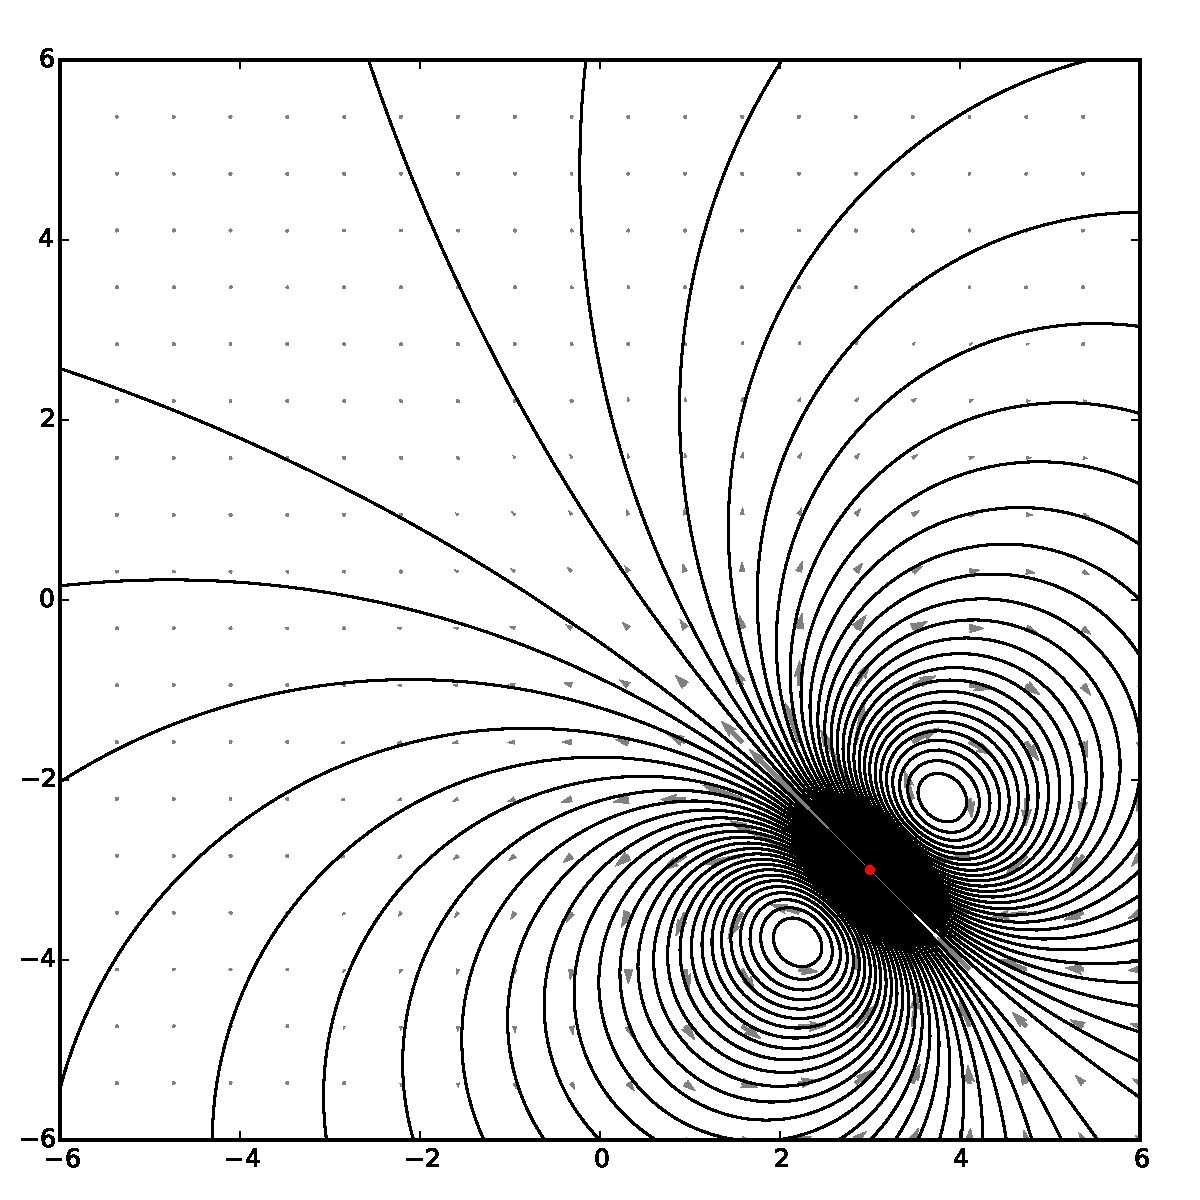
\includegraphics[width = 0.3\textwidth]{./images/singleton_order1/order_1_time_0}
%	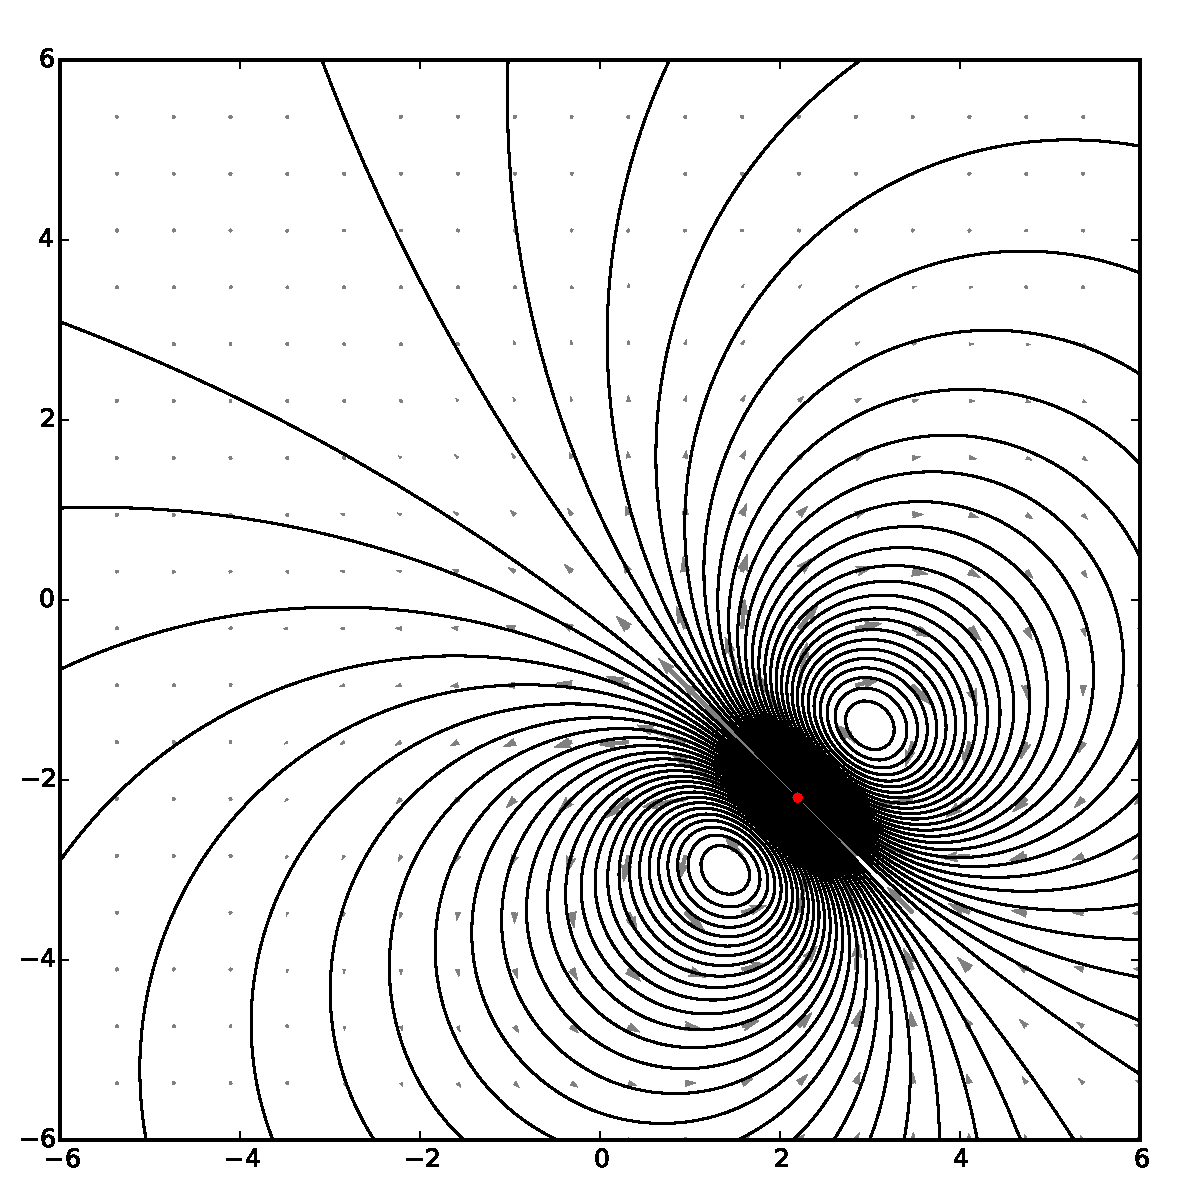
\includegraphics[width = 0.15\textwidth]{./images/singleton_order1/order_1_time_5}
	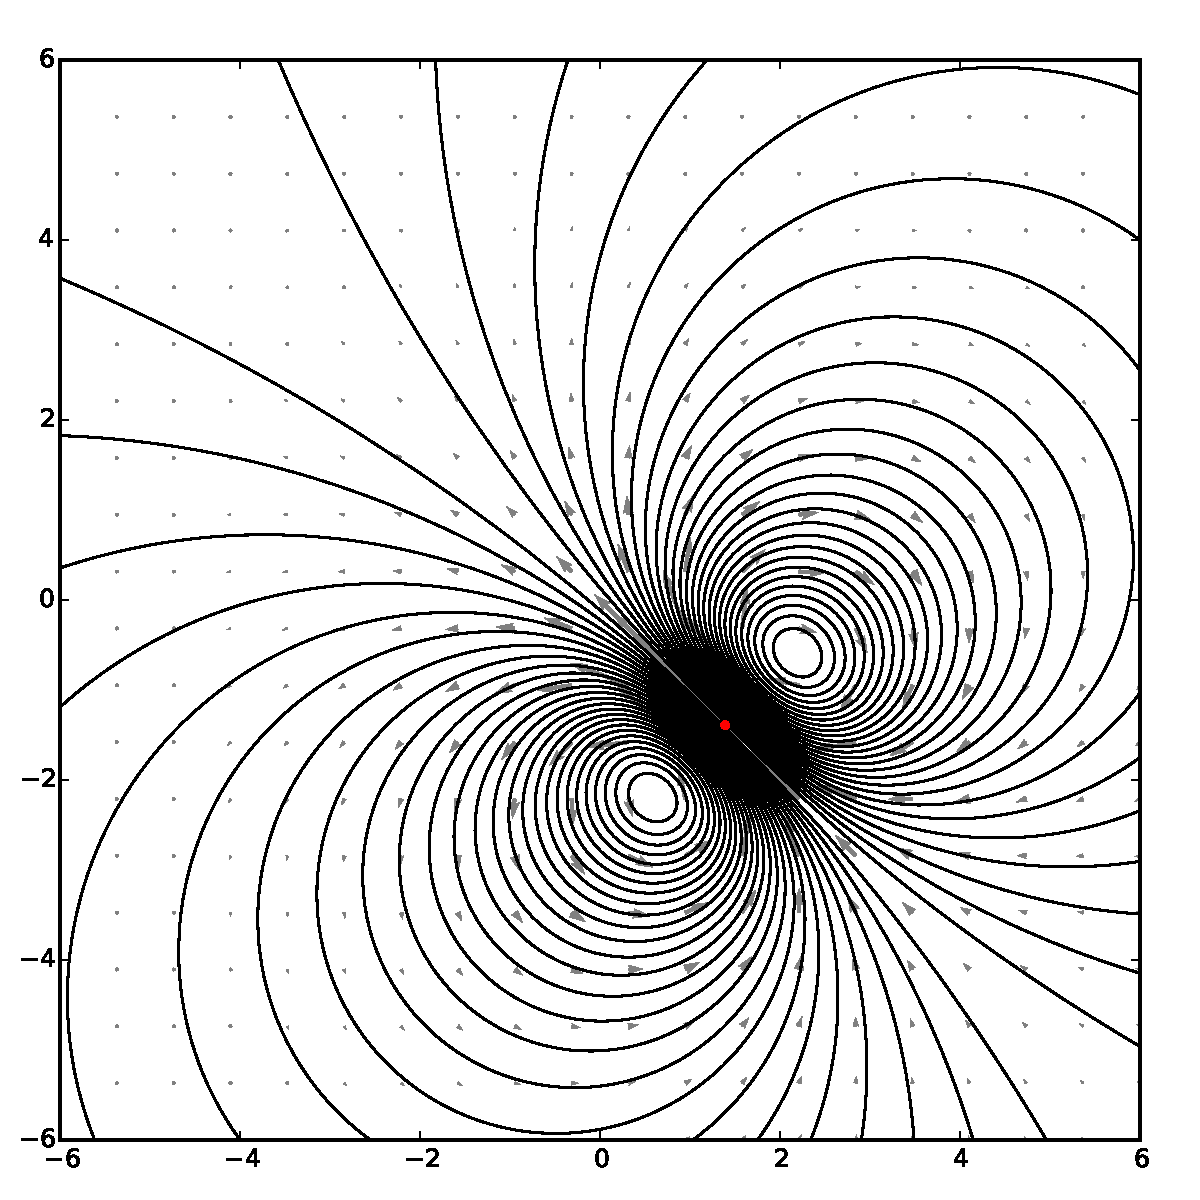
\includegraphics[width = 0.3\textwidth]{./images/singleton_order1/order_1_time_10}
%	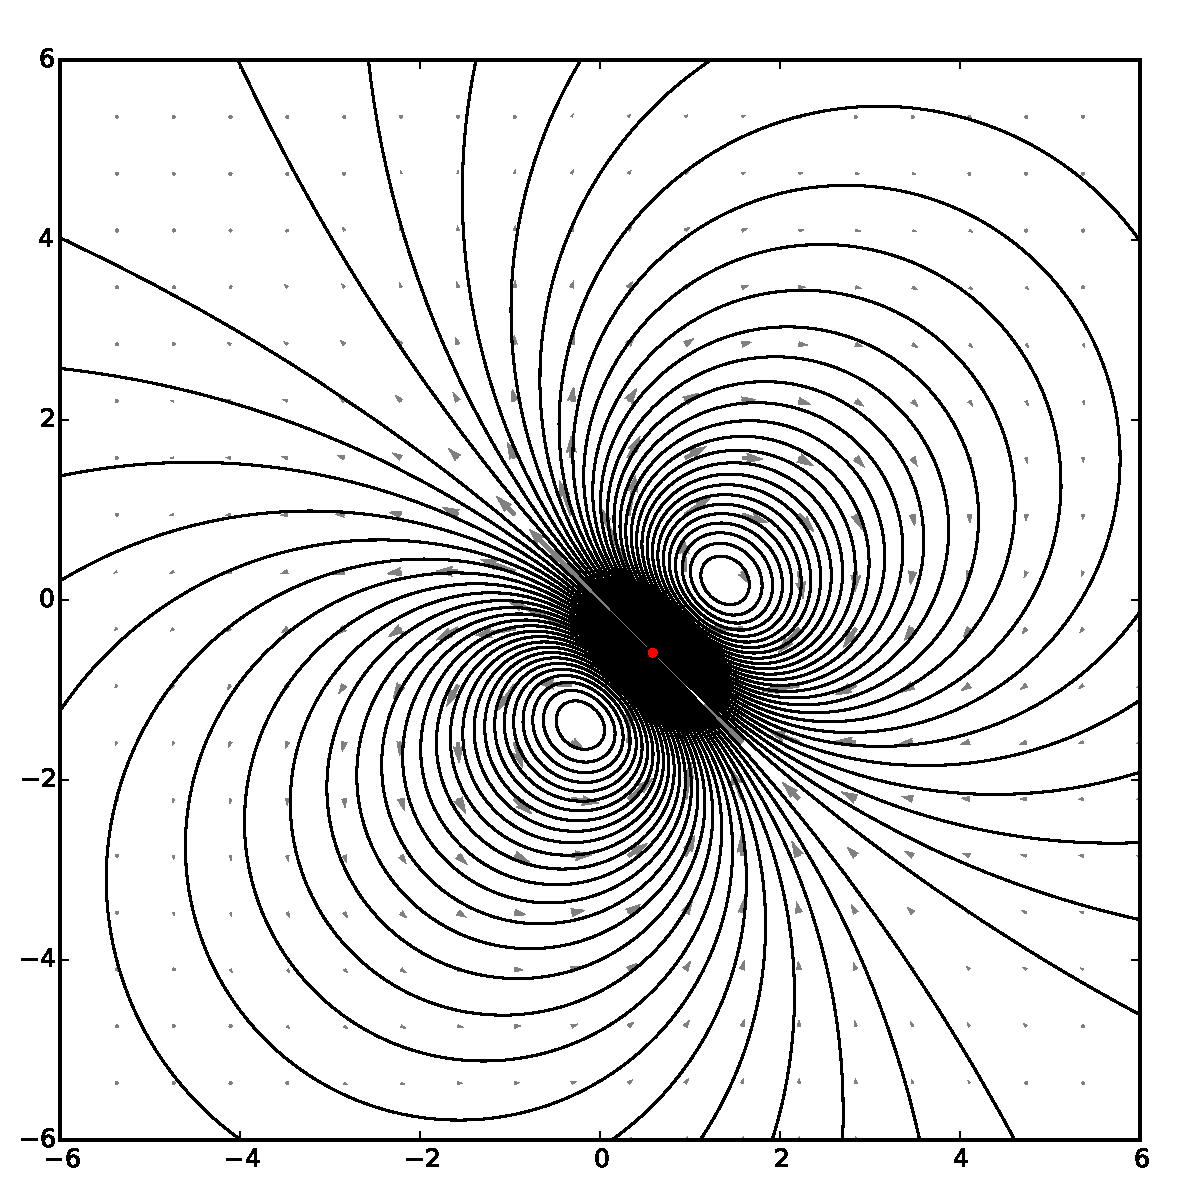
\includegraphics[width = 0.15\textwidth]{./images/singleton_order1/order_1_time_15}
%	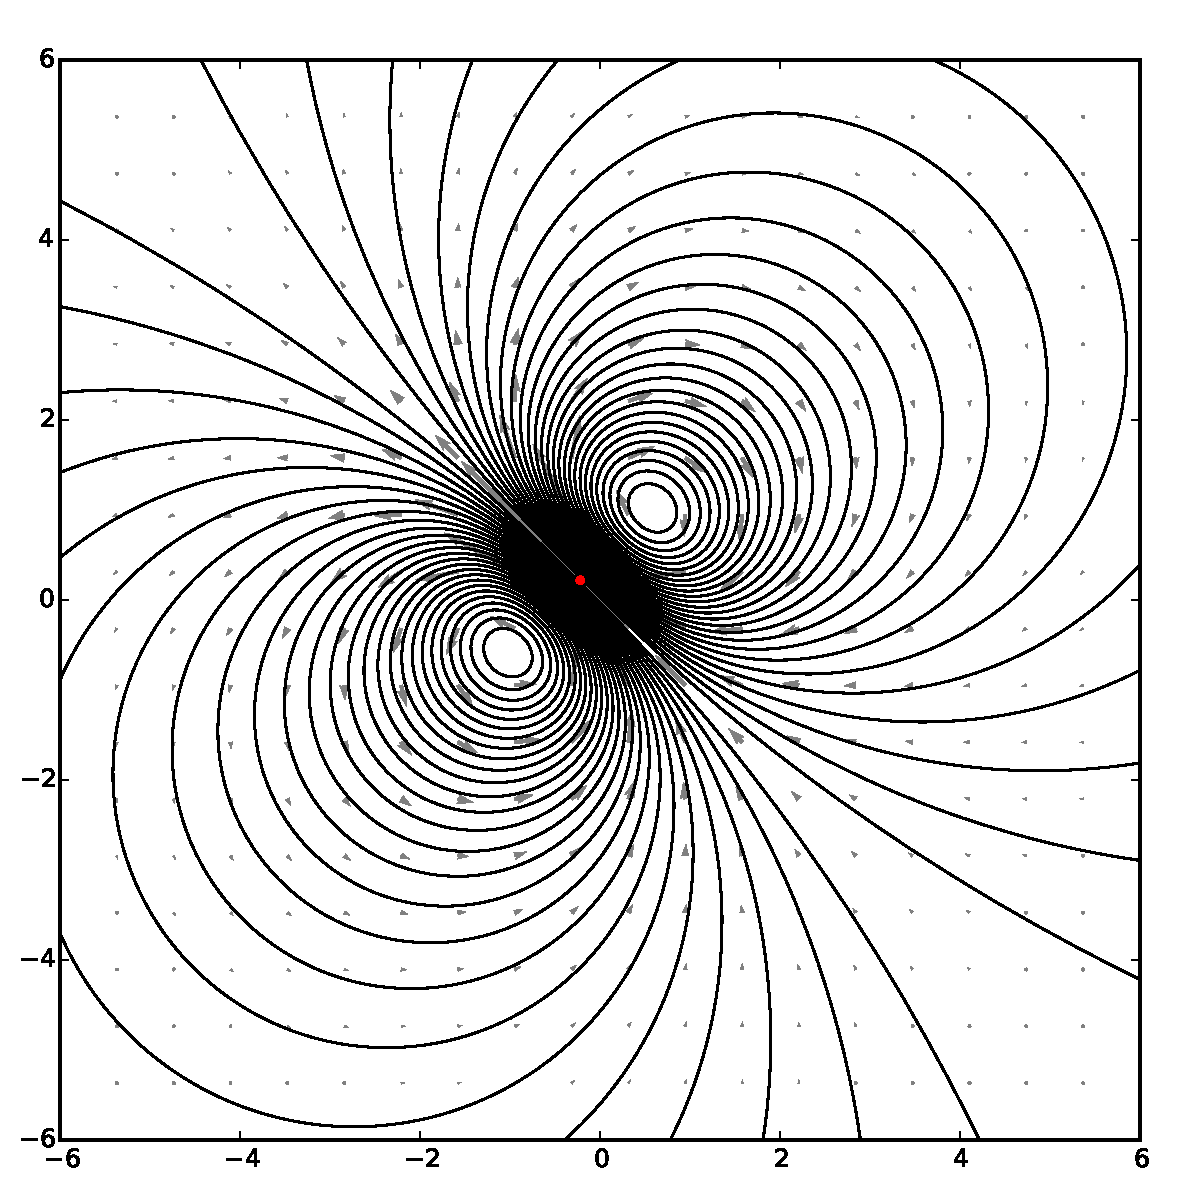
\includegraphics[width = 0.15\textwidth]{./images/singleton_order1/order_1_time_20}
	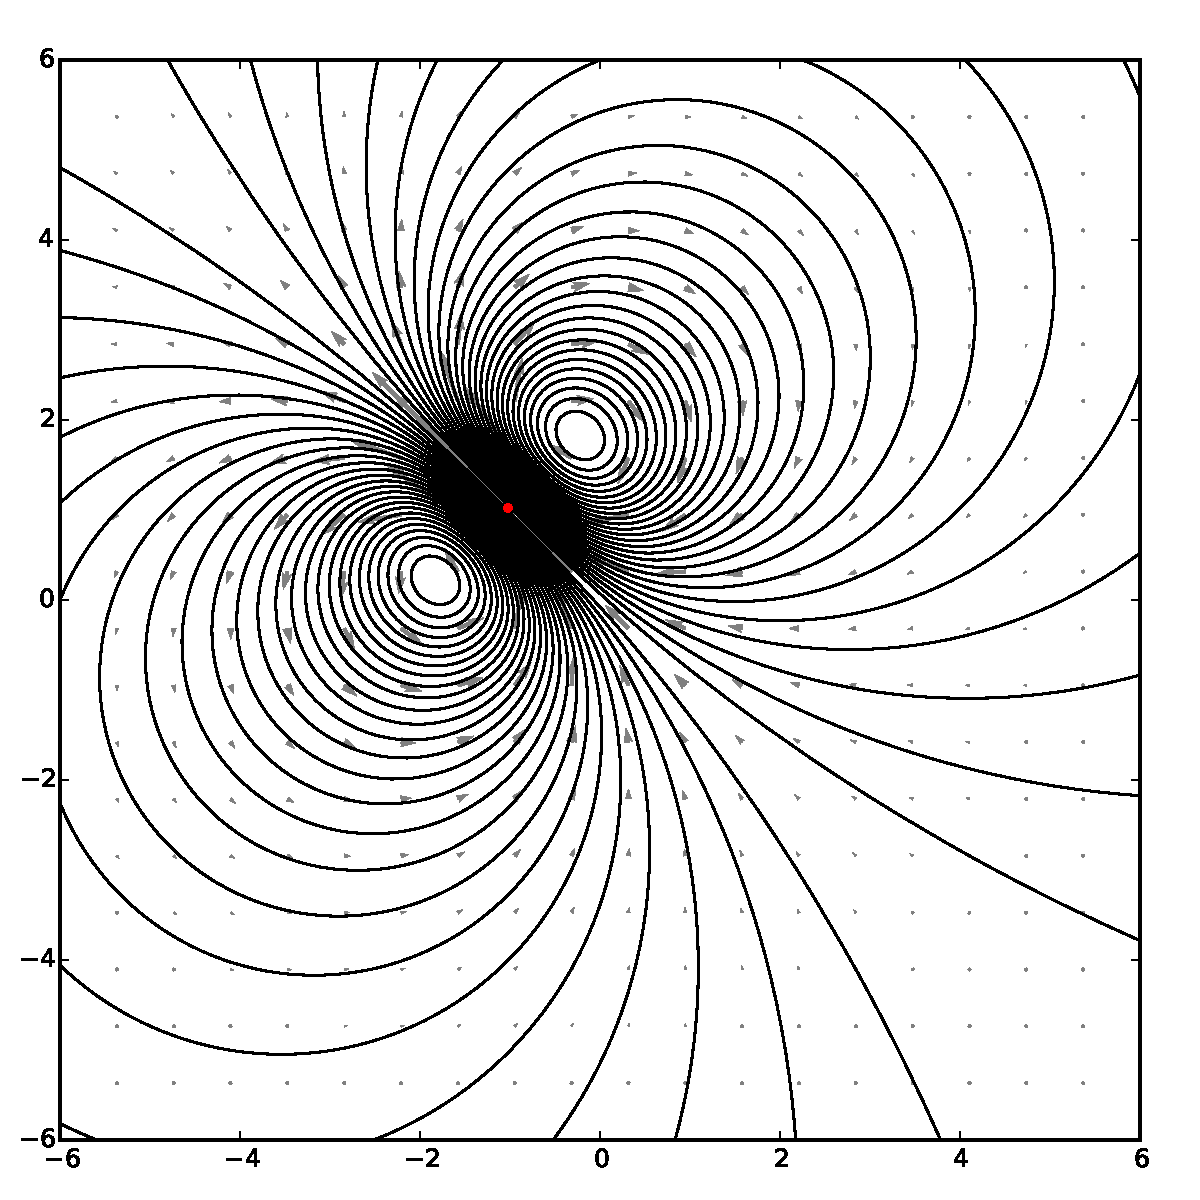
\includegraphics[width = 0.3\textwidth]{./images/singleton_order1/order_1_time_25}
	\caption{A $1$st order jet vortex with initial conditions given by \eqref{eq:ic_order1}
		with snapshots taking at $t=0,10,25$.}
	\label{fig:singleton_order1}
\end{figure}

\subsection{Order 2}
The behavior of a second order vortex does not seem to be explicitly solvable.
Here we consider initial conditions for which 
\begin{align}
	x(0) = 0 \,,\quad\quad y(0) = 0 \,,\quad\quad \Gamma(0)^{xx} = 1 \label{eq:ic_order2}
\end{align}
and all the other circulation variables are initially set to $0$.
The results are depicted in Figure \ref{fig:singleton_order2}.
We observe a structure which rigidly rotates counter-clockwise.

\begin{figure}[h!]
	\centering
	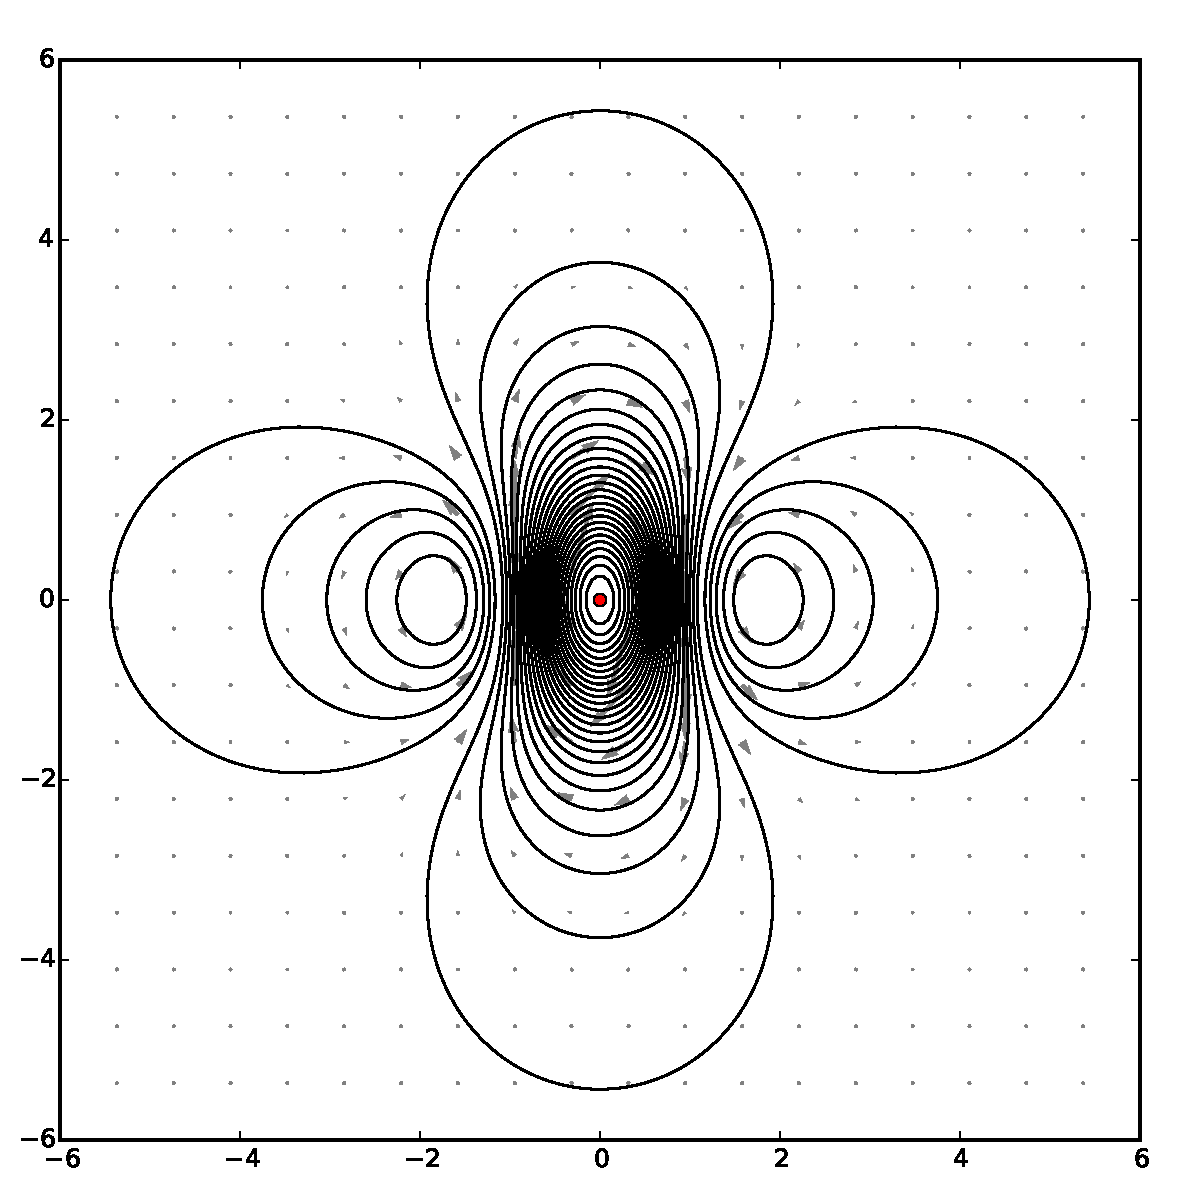
\includegraphics[width = 0.15\textwidth]{./images/singleton_order2/order_2_time_0}
	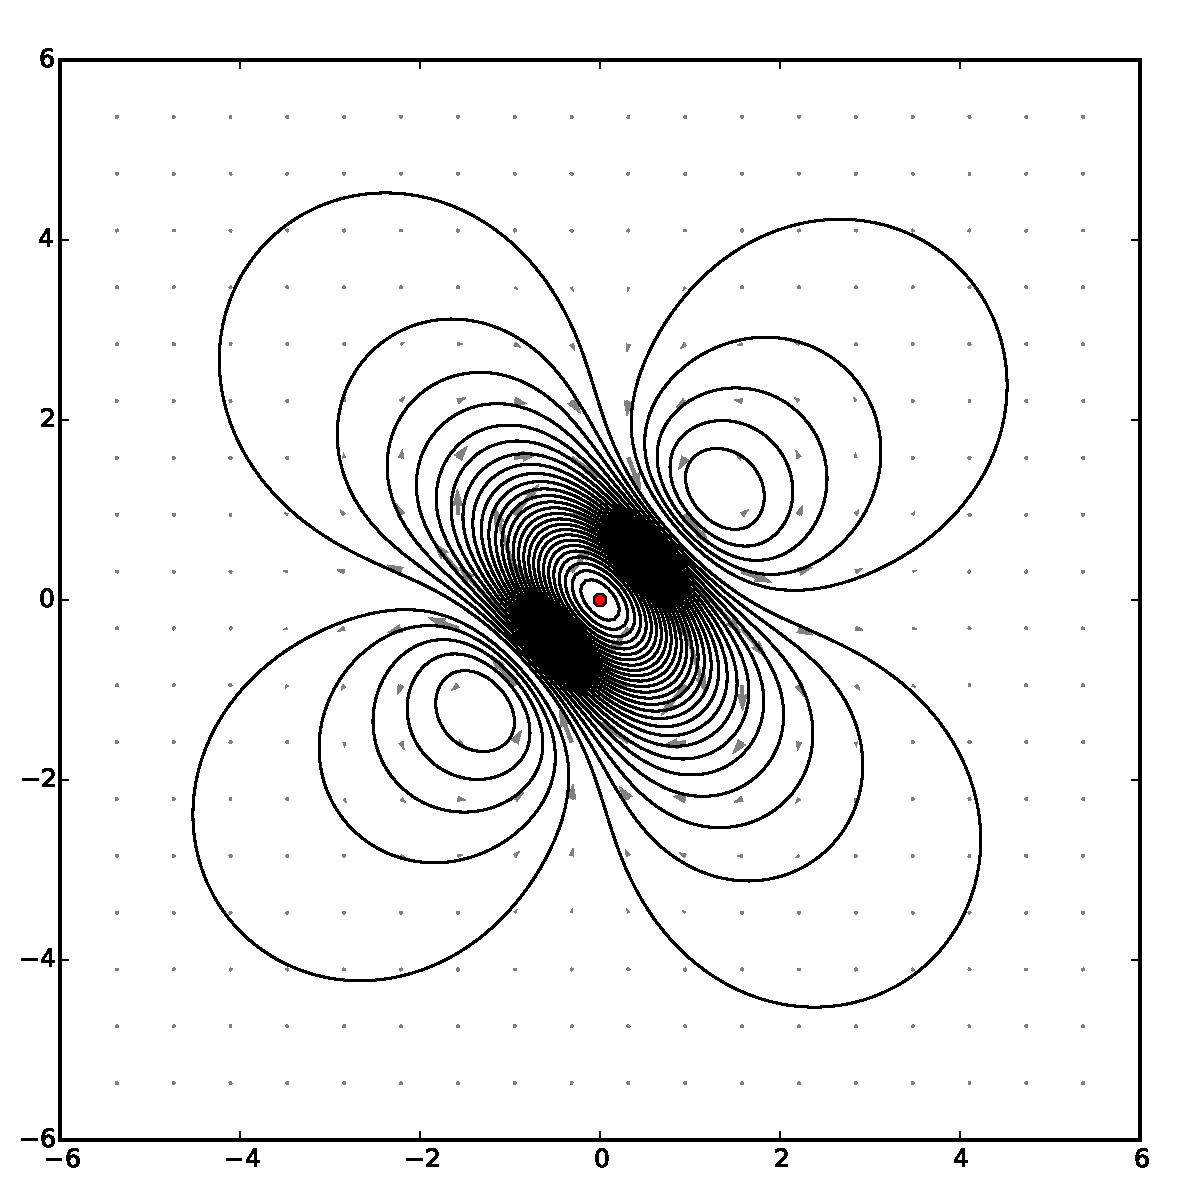
\includegraphics[width = 0.15\textwidth]{./images/singleton_order2/order_2_time_5}
	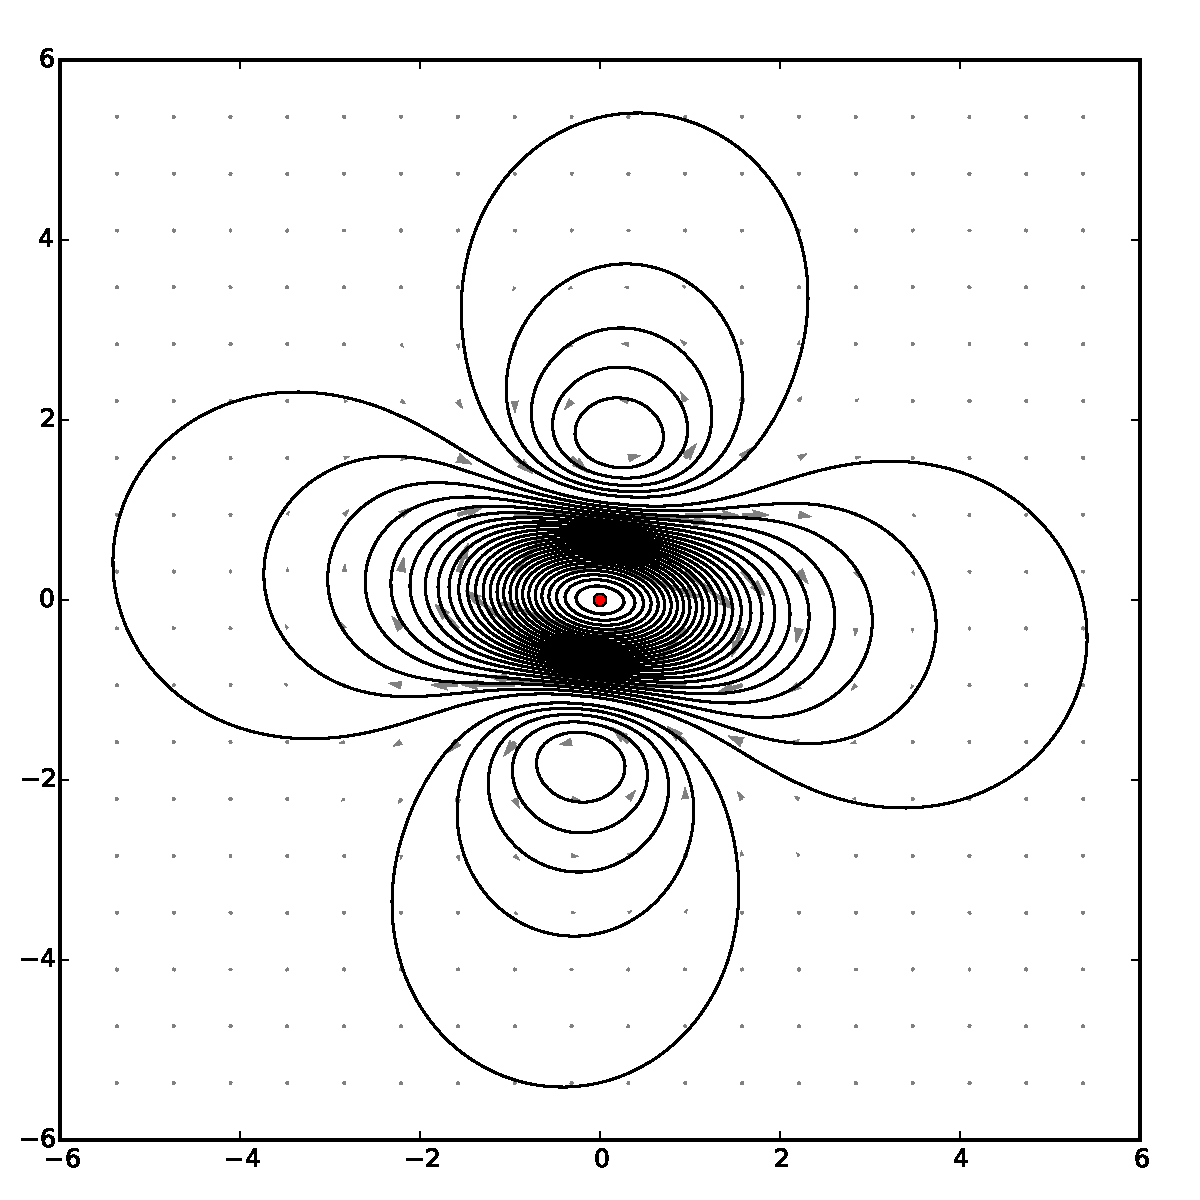
\includegraphics[width = 0.15\textwidth]{./images/singleton_order2/order_2_time_10}
	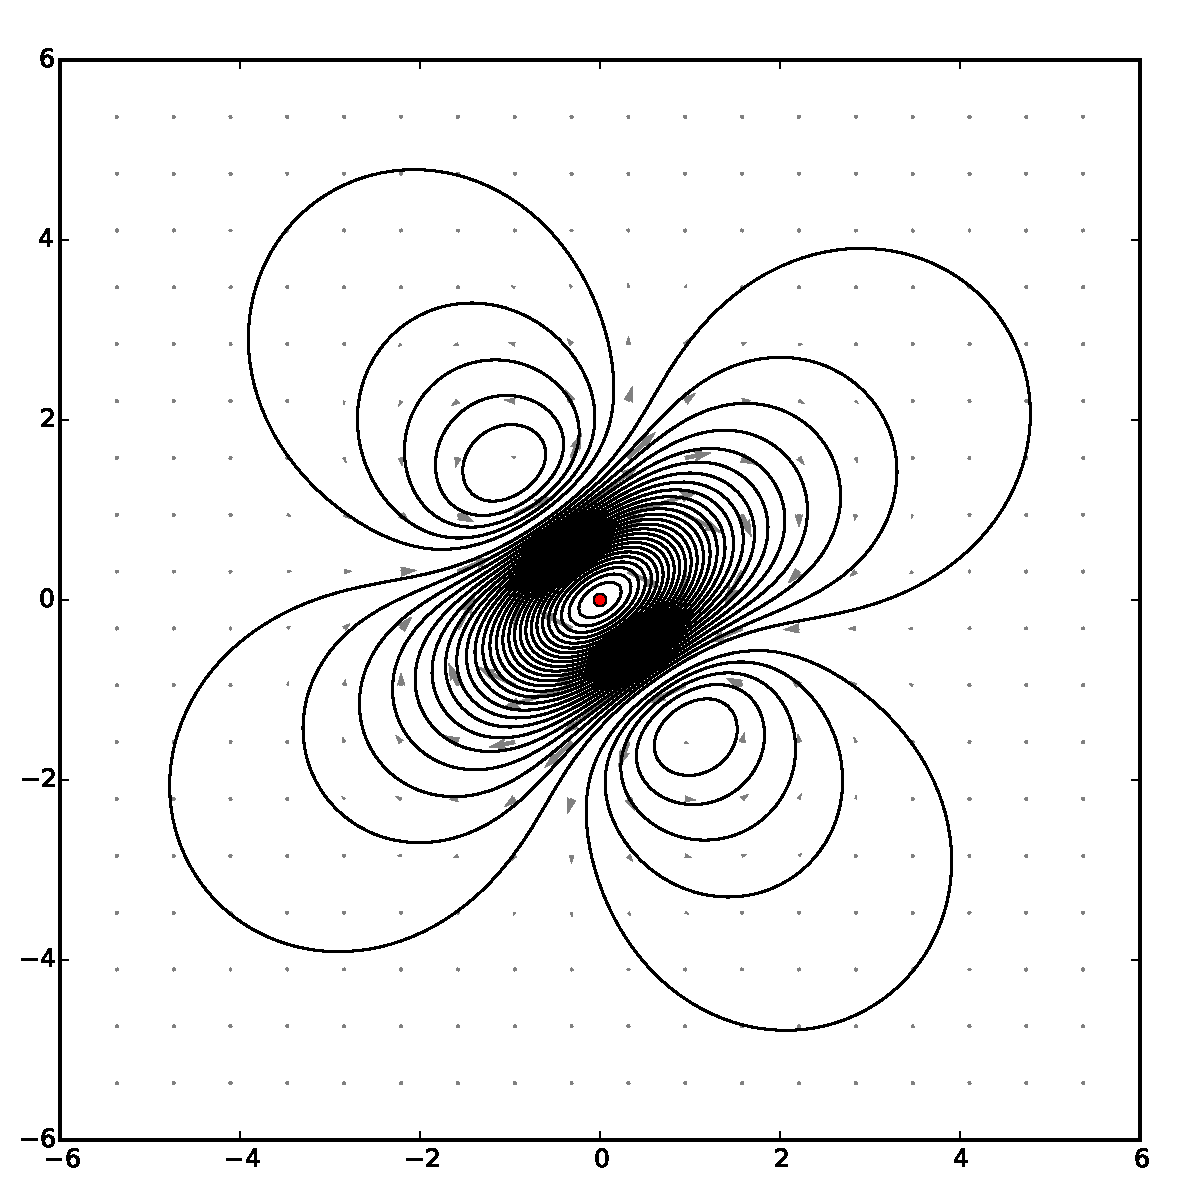
\includegraphics[width = 0.15\textwidth]{./images/singleton_order2/order_2_time_15}
	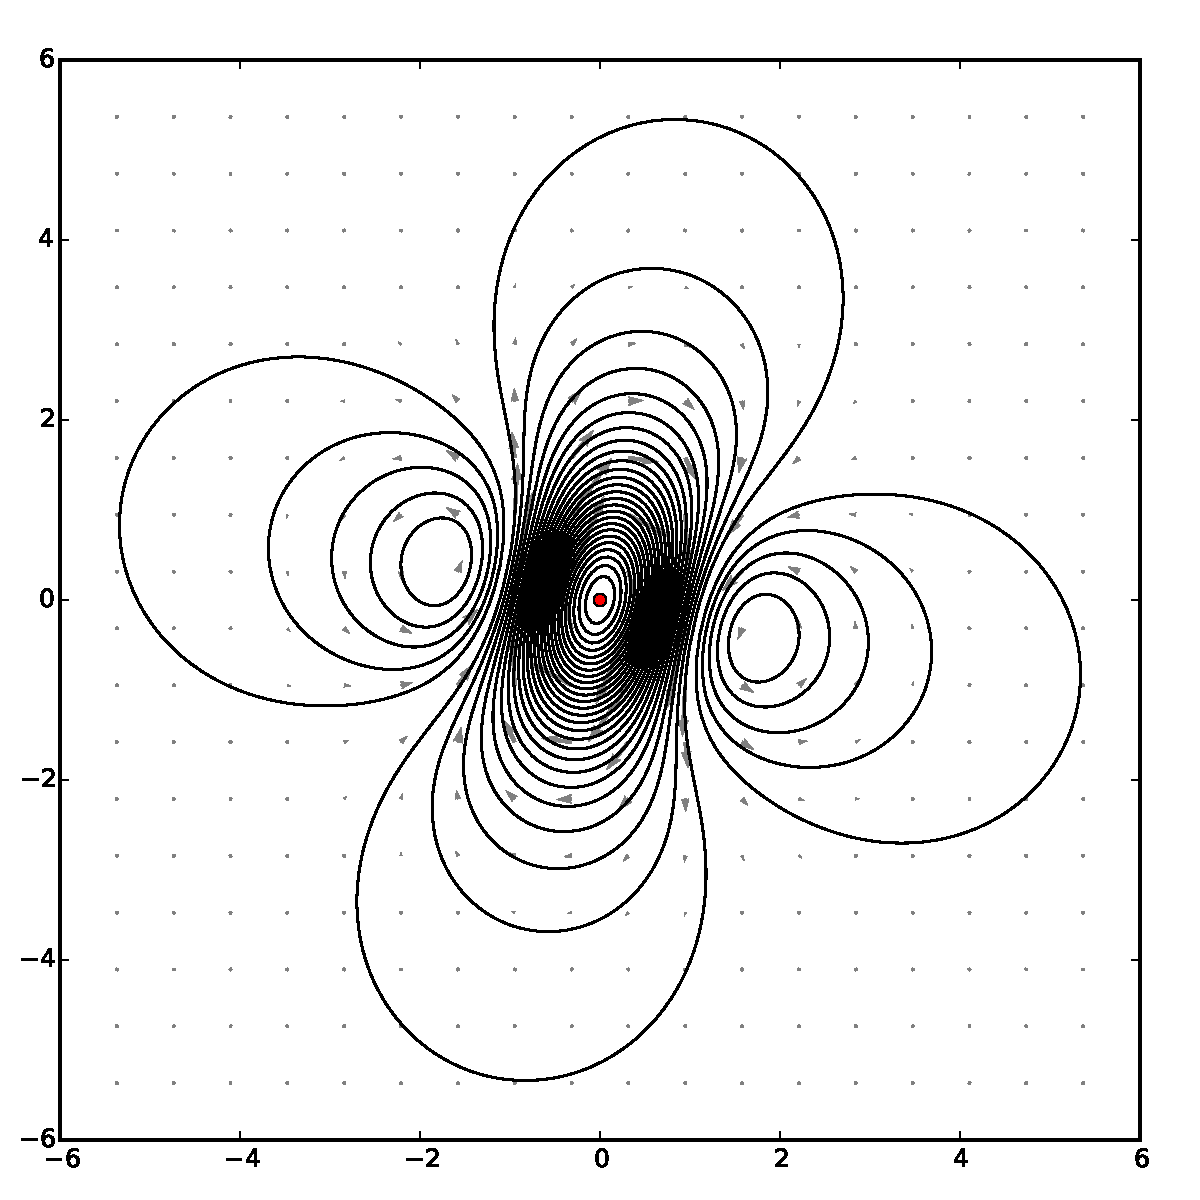
\includegraphics[width = 0.15\textwidth]{./images/singleton_order2/order_2_time_20}
	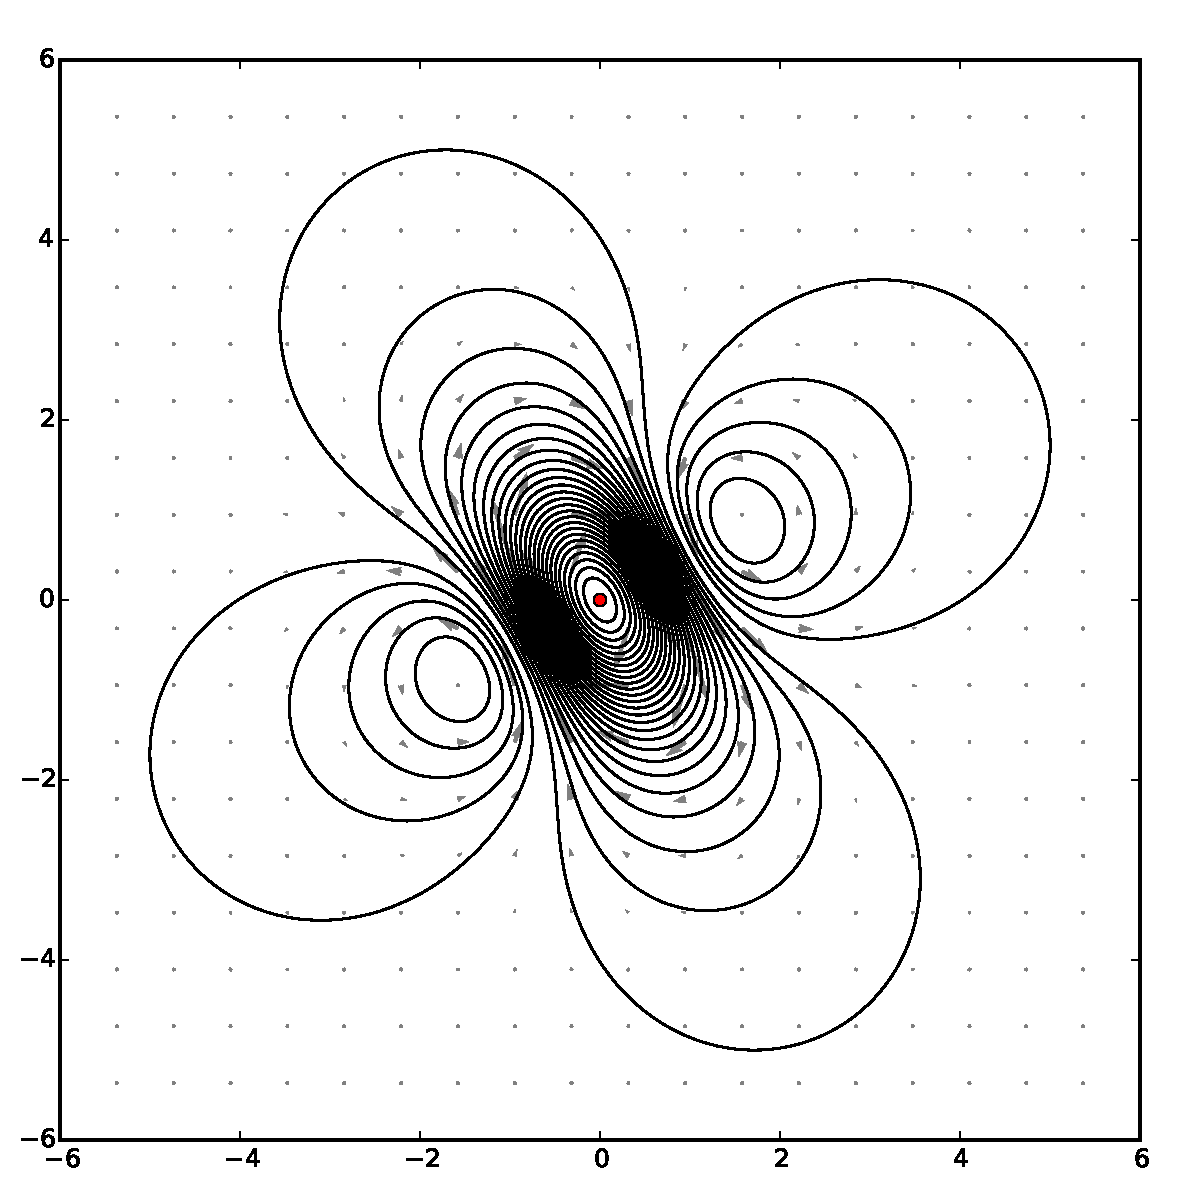
\includegraphics[width = 0.15\textwidth]{./images/singleton_order2/order_2_time_25}
	\caption{A $1$st order jet vortex with initial conditions given by \eqref{eq:ic_order2}
		with snapshots taking at $t=0,5,10,15,20,25$.}
	\label{fig:singleton_order2}
\end{figure}


\subsection{A scattering expiriment}
\label{sec:scattering}
Next we consider two jet vortices.  The first is a first order jet vortex with an initial velocity pointed just slightly above origin.
The second jet vortex is a standard zeroth order vortex located at the origin.
Specificaly, we consider the initial conditions
\begin{align}
	\begin{cases}
	z_0 = (20.0 , \phantom{-}0.25)\quad, \quad \Gamma_0^{0,0} = 0.0 \quad,\quad \Gamma_0^{1,0} = 0.0 \quad,\quad \Gamma_0^{0,1} = -1.0 \\
	z_1 = (\phantom{2}0.0 , -0.25)\quad, \quad \Gamma_0^{0,0} = 1.0 \quad,\quad \Gamma_0^{1,0} = 0.0 \quad,\quad \Gamma_0^{0,1} = \phantom{-}0.0
	\end{cases}
	\label{eq:ic}
\end{align}
with $\Gamma_i^{mn} = 0$ for $m+n > 1$ and $i=0,1$.
The vortex at the origin appears to remain at the origin throughout the numerical run ($t=0$ to $t=150$).
The first order jet vortex starts by moving to the left in a straightline until it comes into proximity of the zeroth order vortex.
Then the first order jet vortex swings around the the zeroth order vortex, traversing an angle of roughly 30 degrees
before zooming off into the lower left quadrant of the plane in a straight line.  These results are depicted in Figure \ref{fig:scatter}

\begin{figure}[h!]
	\centering
	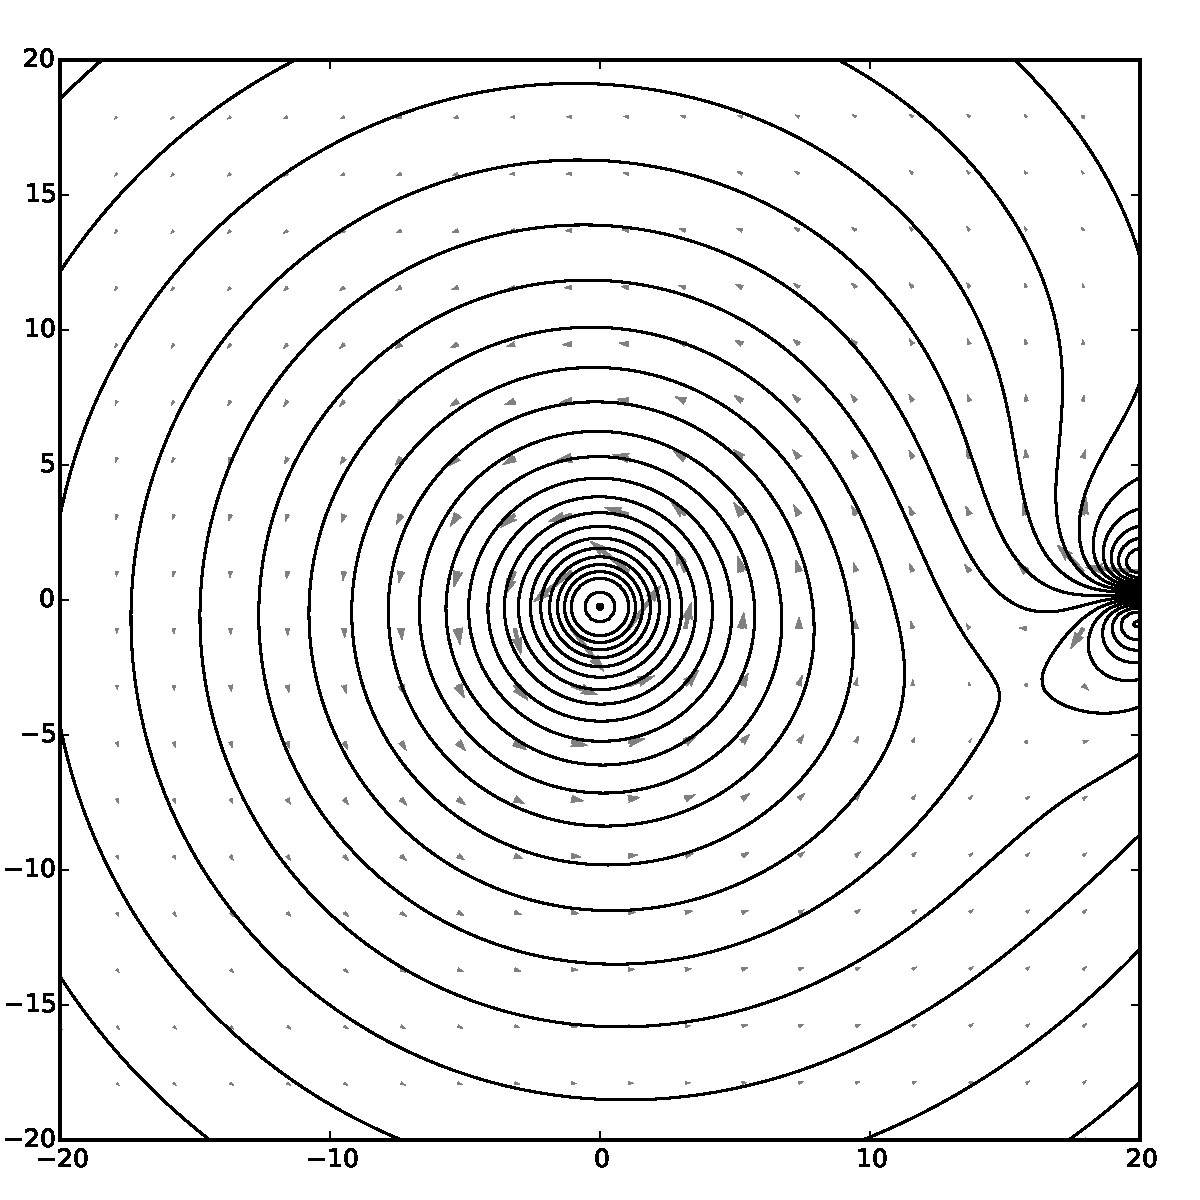
\includegraphics[width=0.3\textwidth]{./images/scattering/frame_time_0}
	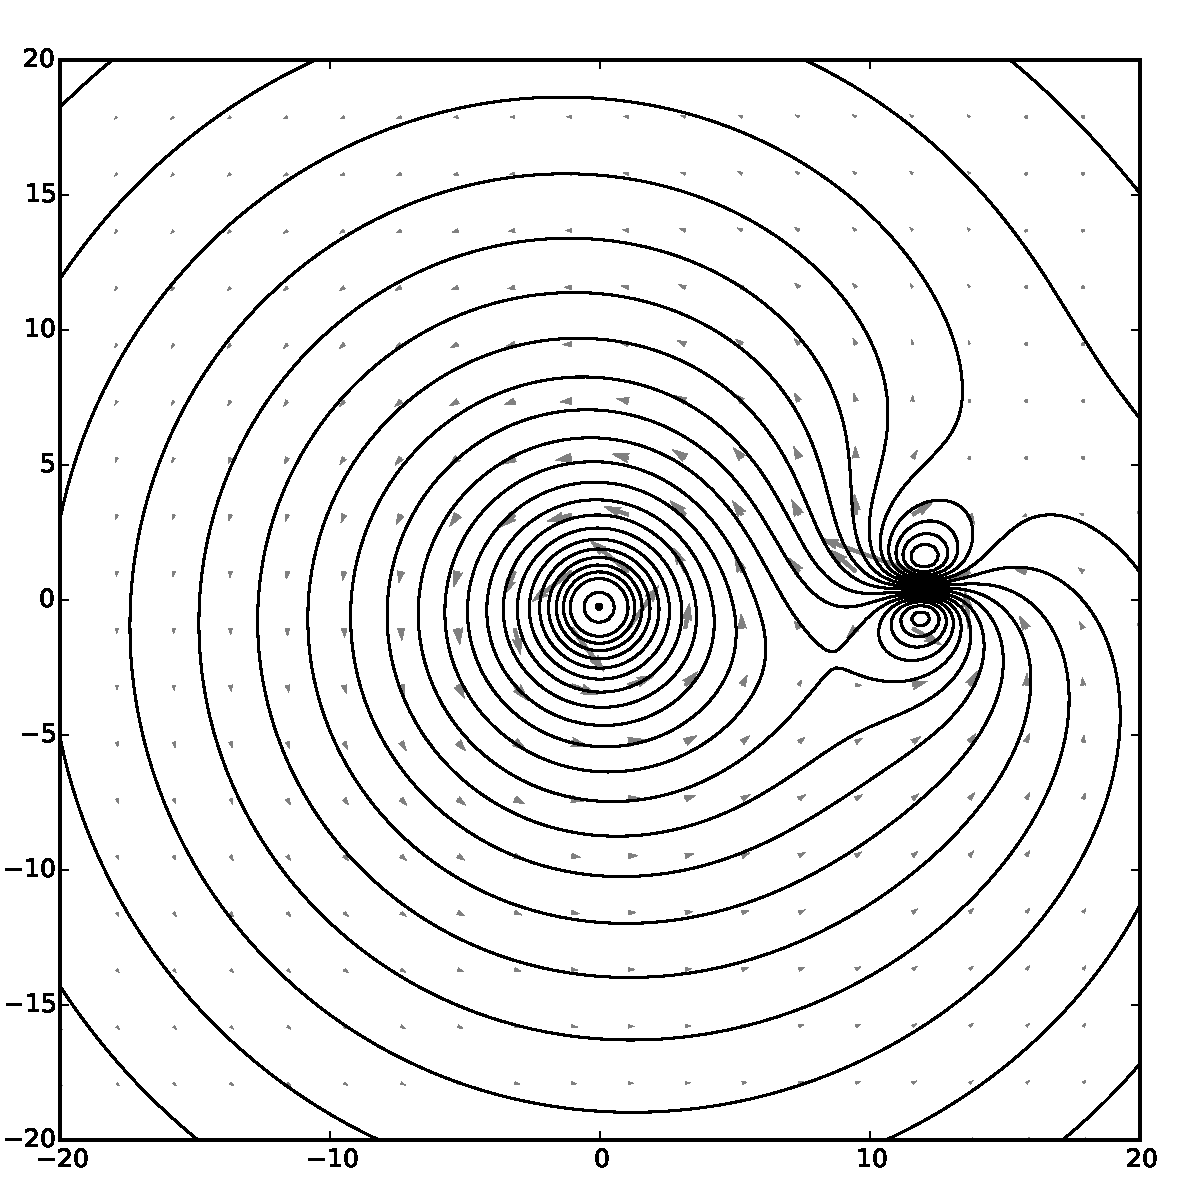
\includegraphics[width=0.3\textwidth]{./images/scattering/frame_time_25}
	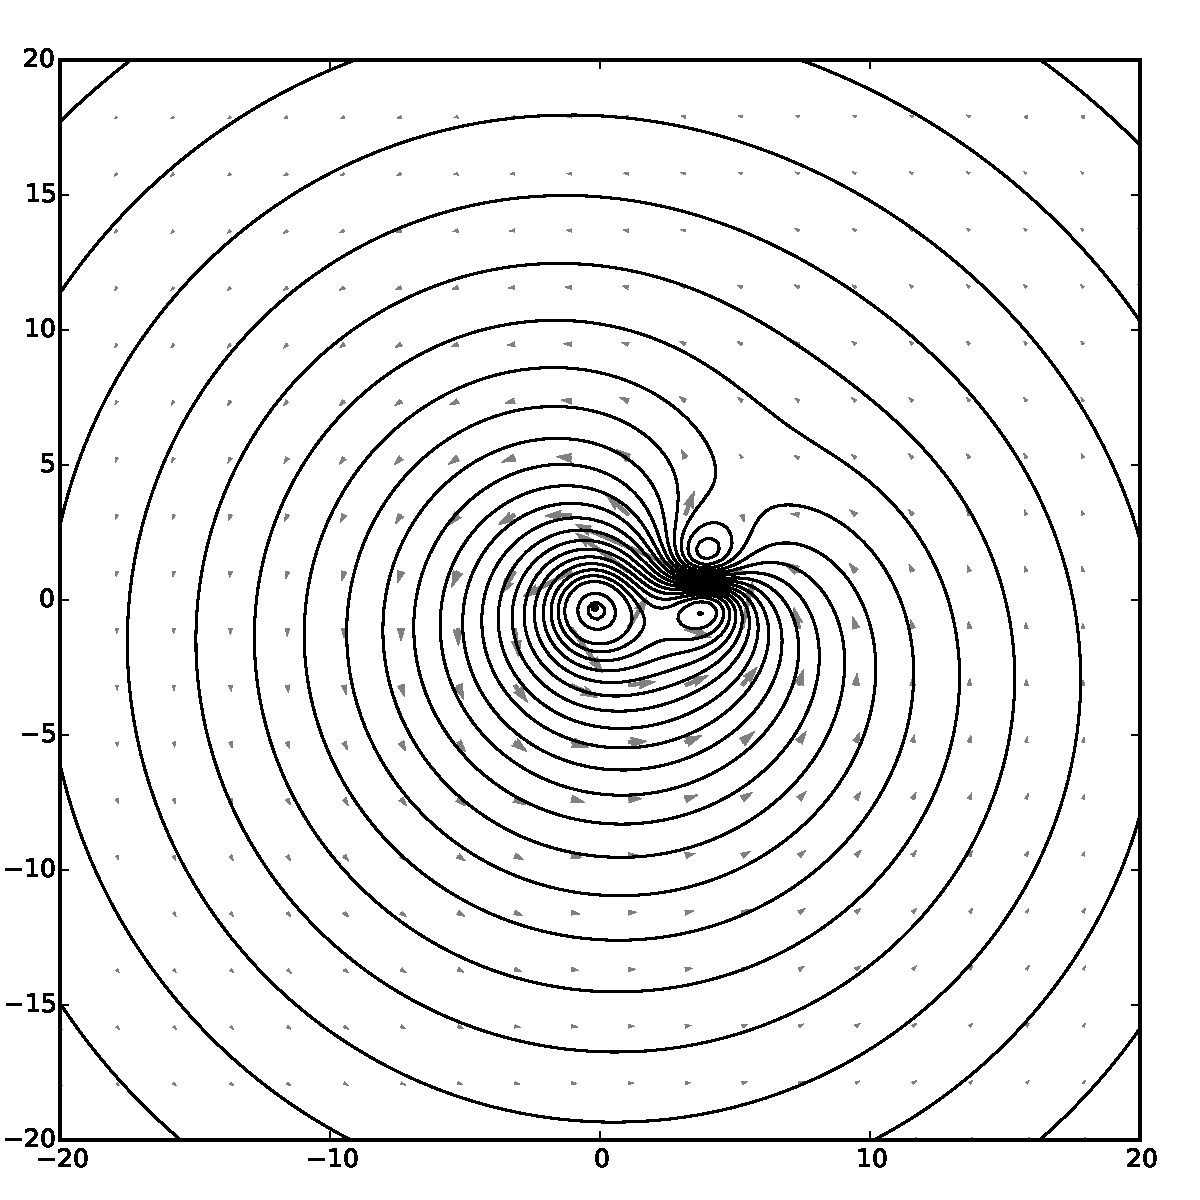
\includegraphics[width=0.3\textwidth]{./images/scattering/frame_time_50}
	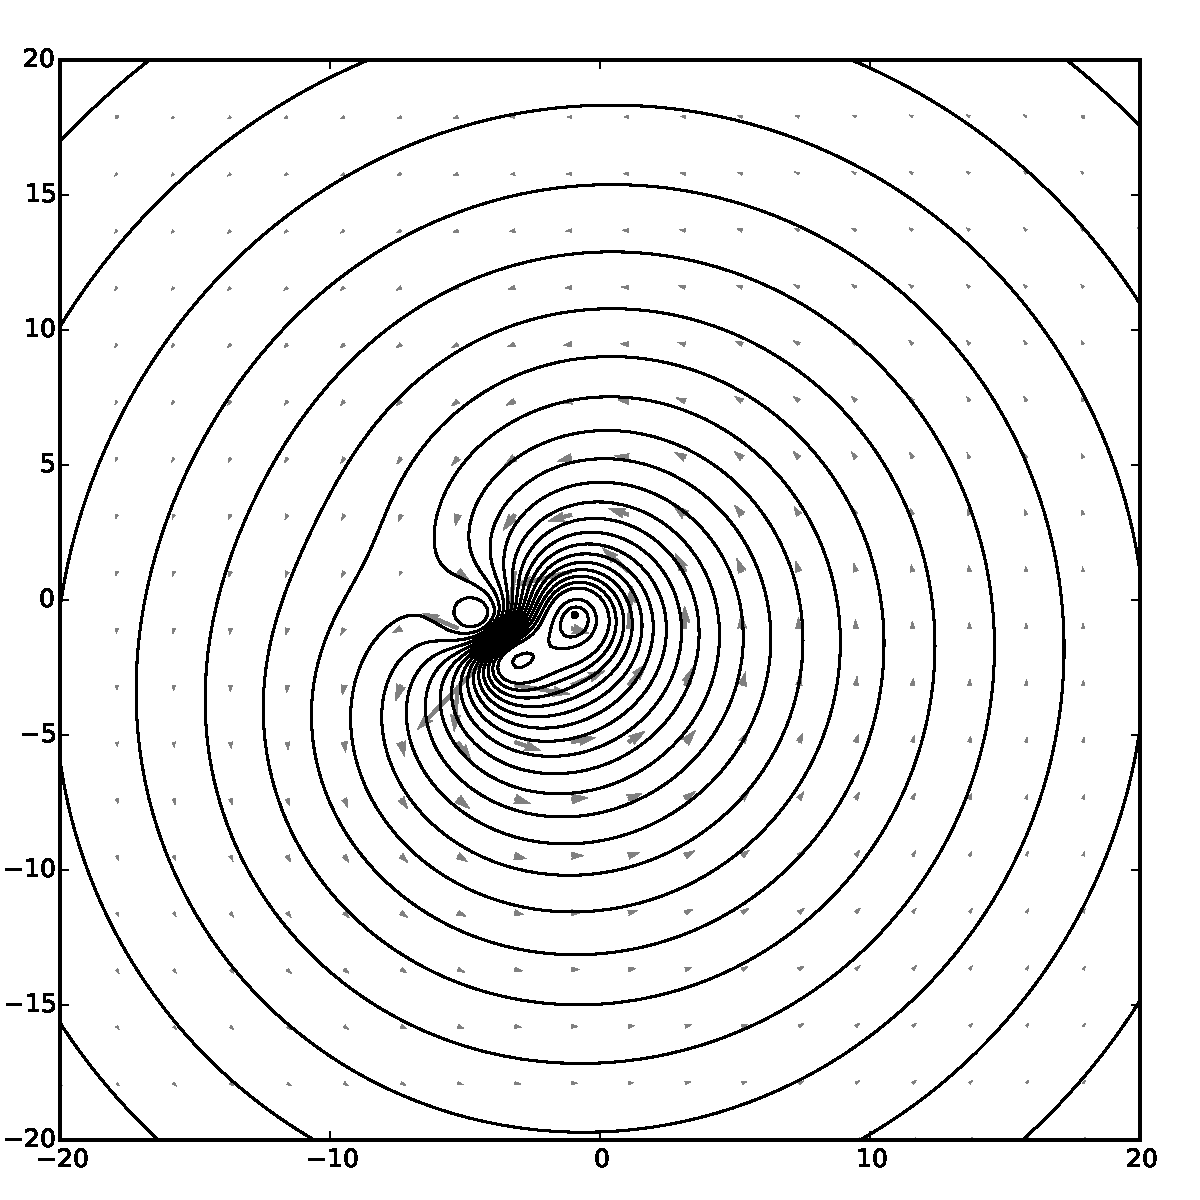
\includegraphics[width=0.3\textwidth]{./images/scattering/frame_time_75}
	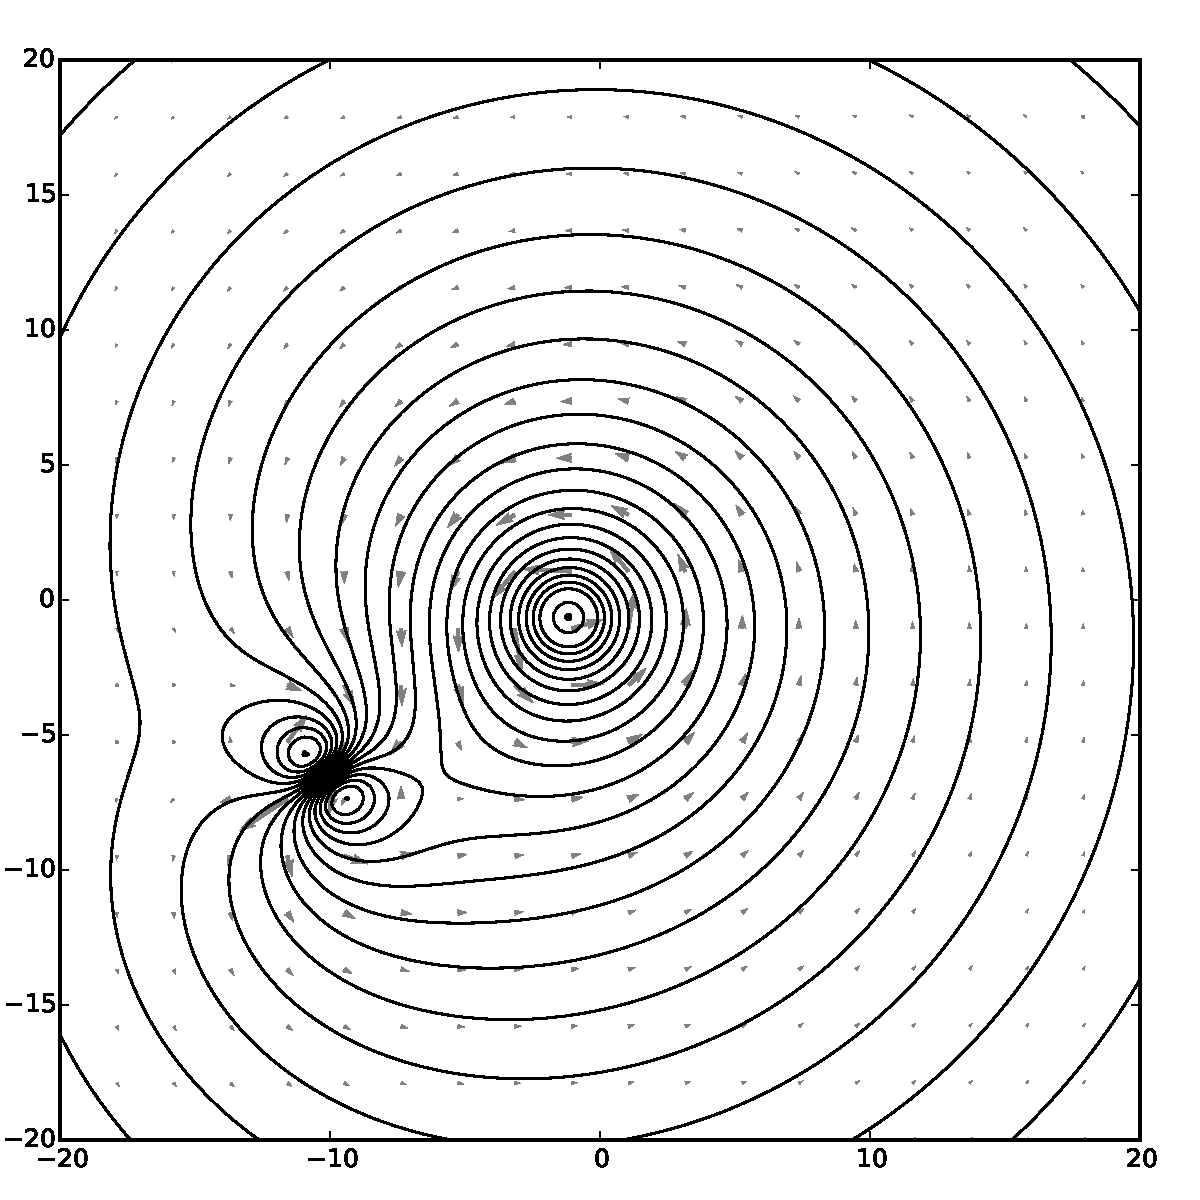
\includegraphics[width=0.3\textwidth]{./images/scattering/frame_time_101}
	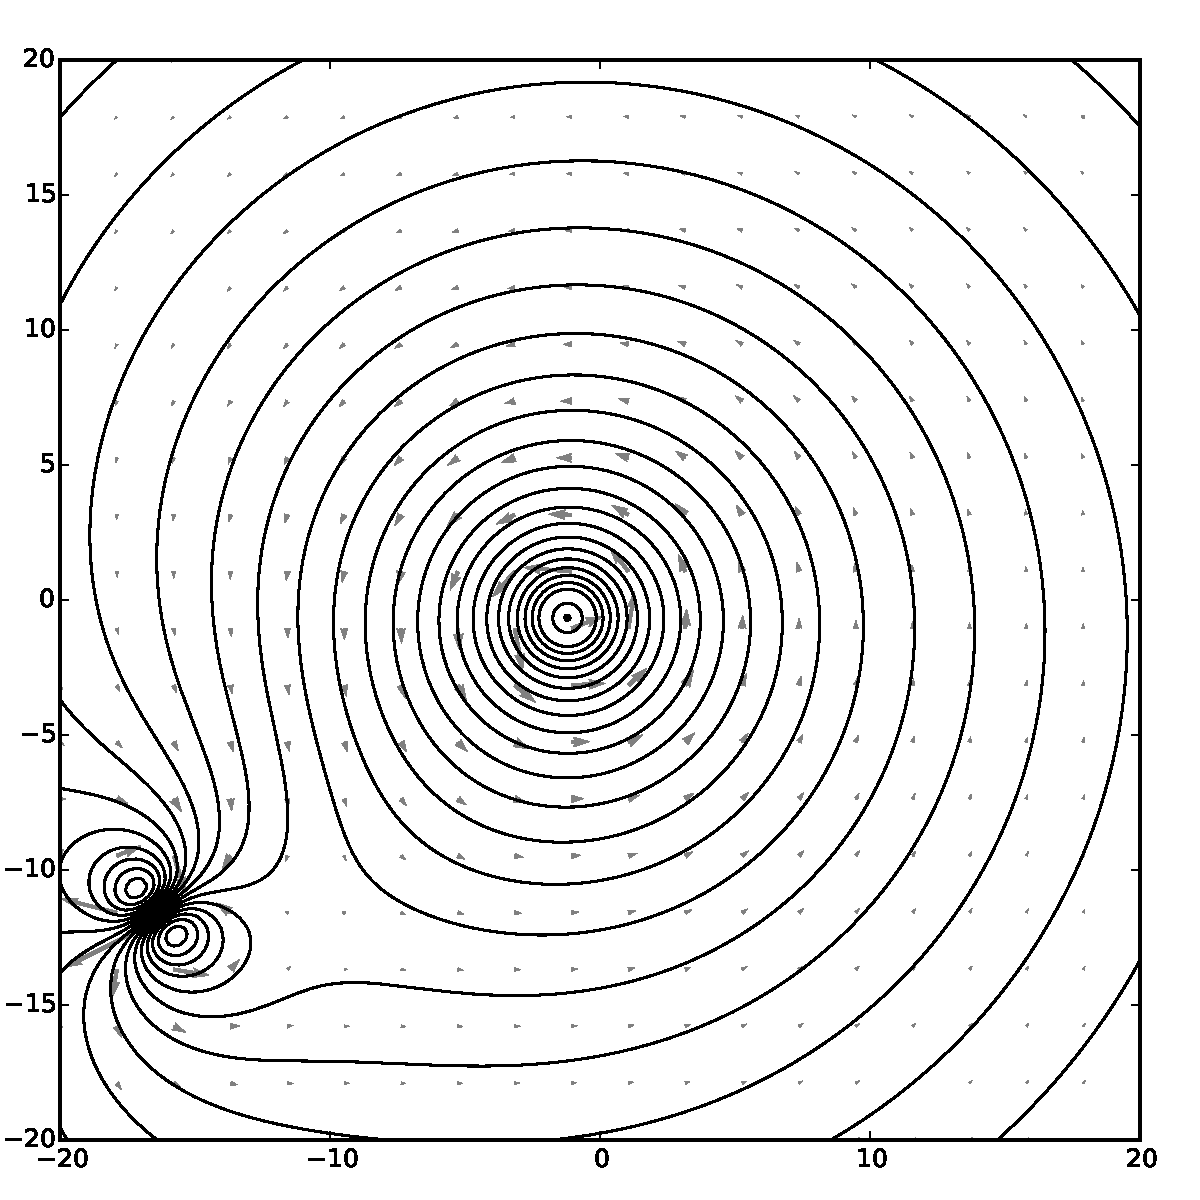
\includegraphics[width=0.3\textwidth]{./images/scattering/frame_time_126}
	\caption{A numerical run is shown with mirror image initial conditions for two 1st order jet vortices, as given in \eqref{eq:ic}.
		From left to right and top to bottom these are snapshots at times $t=0,25,50,75,100,125$ respectively.}
	\label{fig:scatter}
\end{figure}

\subsection{The method of images}
\label{sec:method_of_images}
Here we incorporate first order jet vortices into the method of images\todo{Cite something}.
We consider the initial conditions consisting of two first order jet vortices which are mirror images of each other with respect to the $x$-axis.
By symmetry, the resulting vector-field should be tangential to the $x$-axis, and provides a means of considering a boundary that satisfied the no-penetration condition.
Specifically, we consider the initial condition:
\begin{align}
	\begin{cases}
	z_0 = (1.5 , \phantom{-}1.5)\quad, \quad \Gamma_0^{0,0} = \phantom{-}0.5 \quad,\quad \Gamma_0^{1,0} = \phantom{-}0.5 \quad,\quad \Gamma_0^{0,1} = 1.5 \\
	z_1 = (1.5,-1.5)\quad, \quad \Gamma_0^{0,0} = -0.5 \quad,\quad \Gamma_0^{1,0} = -0.5 \quad,\quad \Gamma_0^{0,1} =1.5
	\end{cases}
	\label{eq:ic moi}
\end{align}
with $\Gamma_i^{mn} = 0$ for $m+n > 1$ and $i=0,1$.

The resulting dynamics depicted in Figure \ref{fig:moi} shows that as a first order jet vortex approaches a boundary it will turn its motion along the boundary and then move away so that its angle of reflection equals its angle of incidence. 

\begin{figure}[h!]
	\centering
	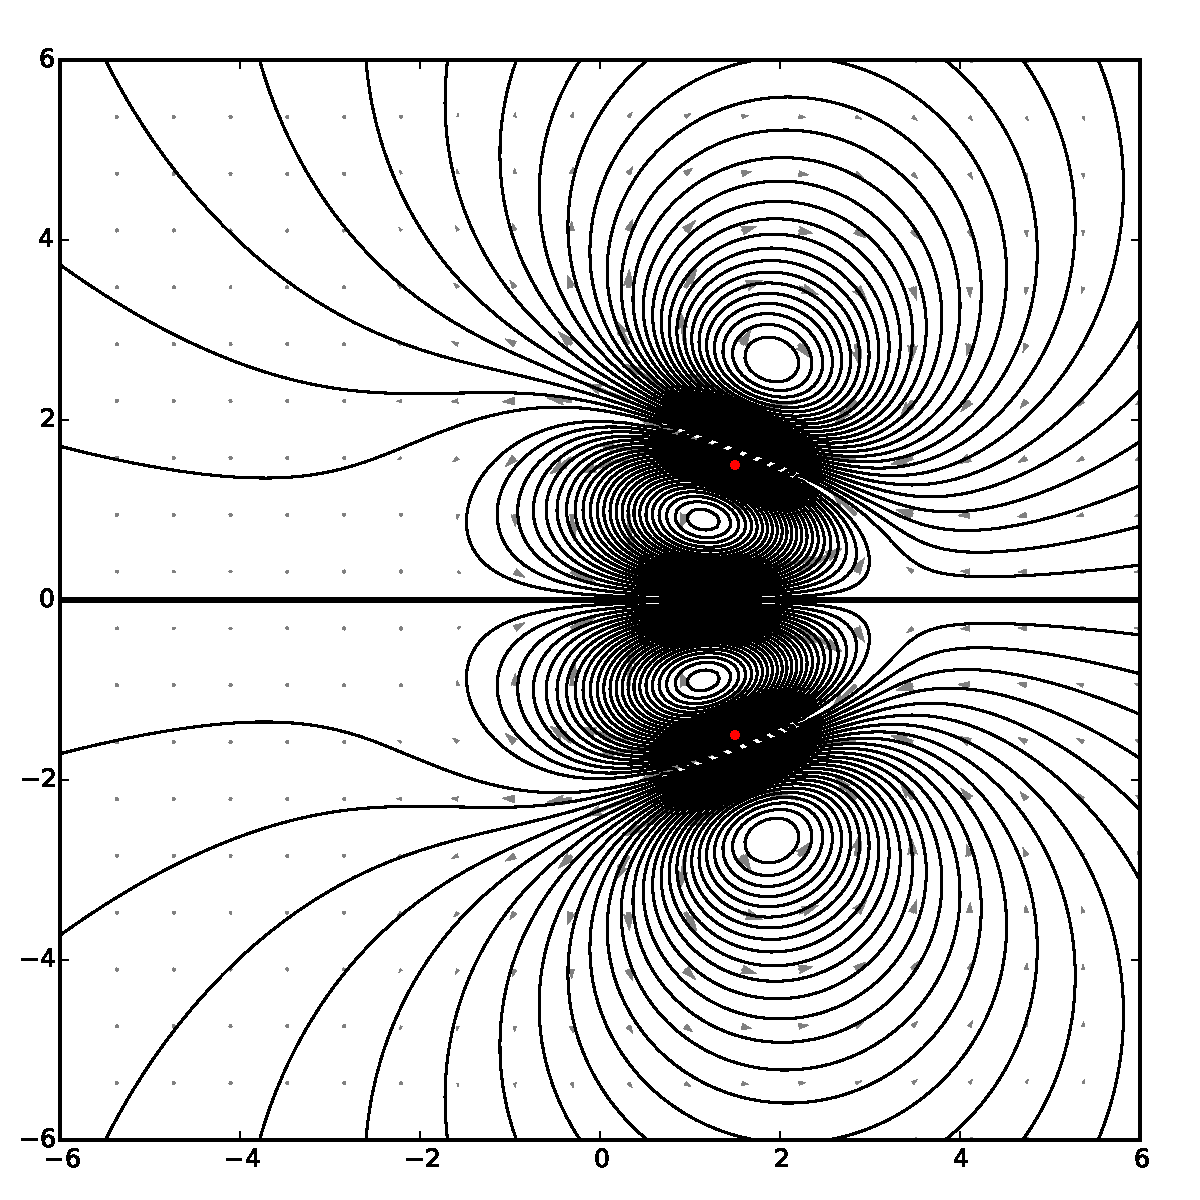
\includegraphics[width=0.3\textwidth]{./images/moi_frames/time_0}
	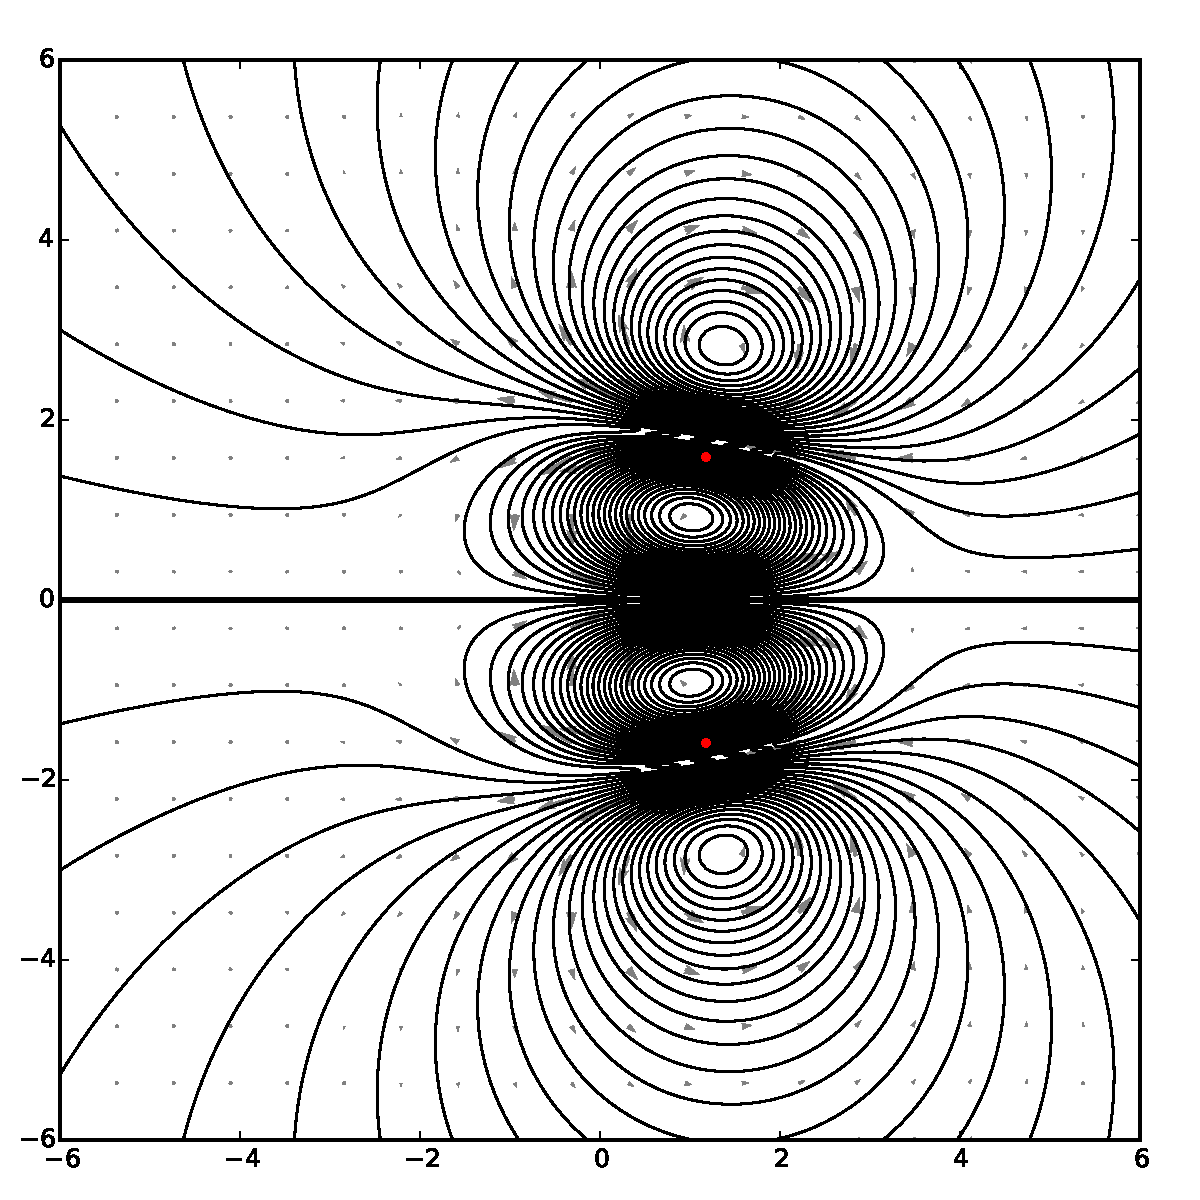
\includegraphics[width=0.3\textwidth]{./images/moi_frames/time_1p7}
	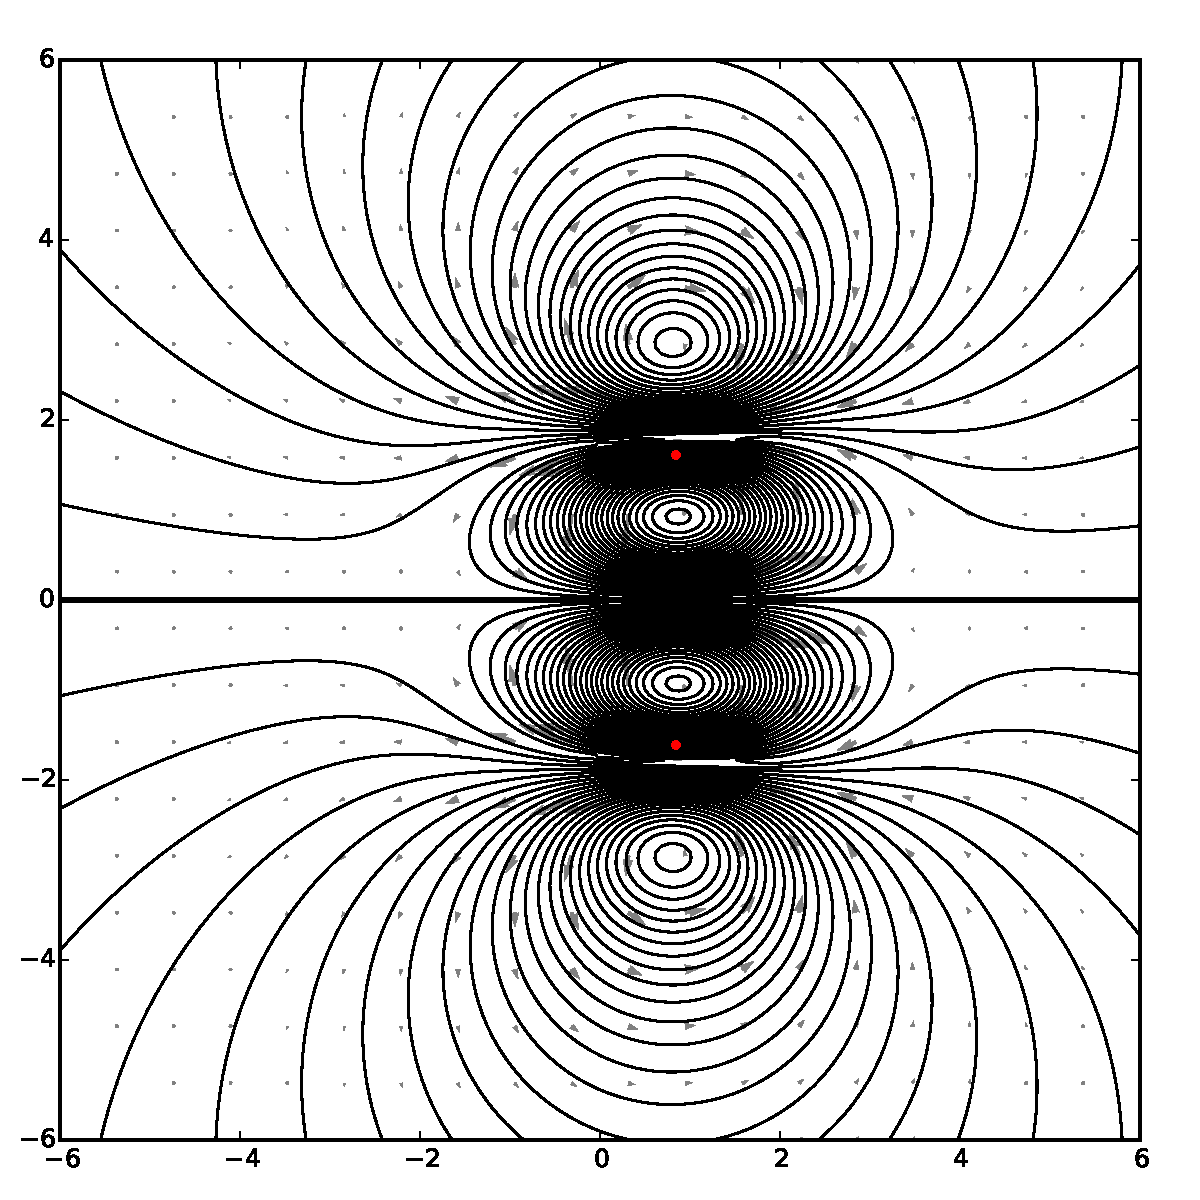
\includegraphics[width=0.3\textwidth]{./images/moi_frames/time_3p4}
	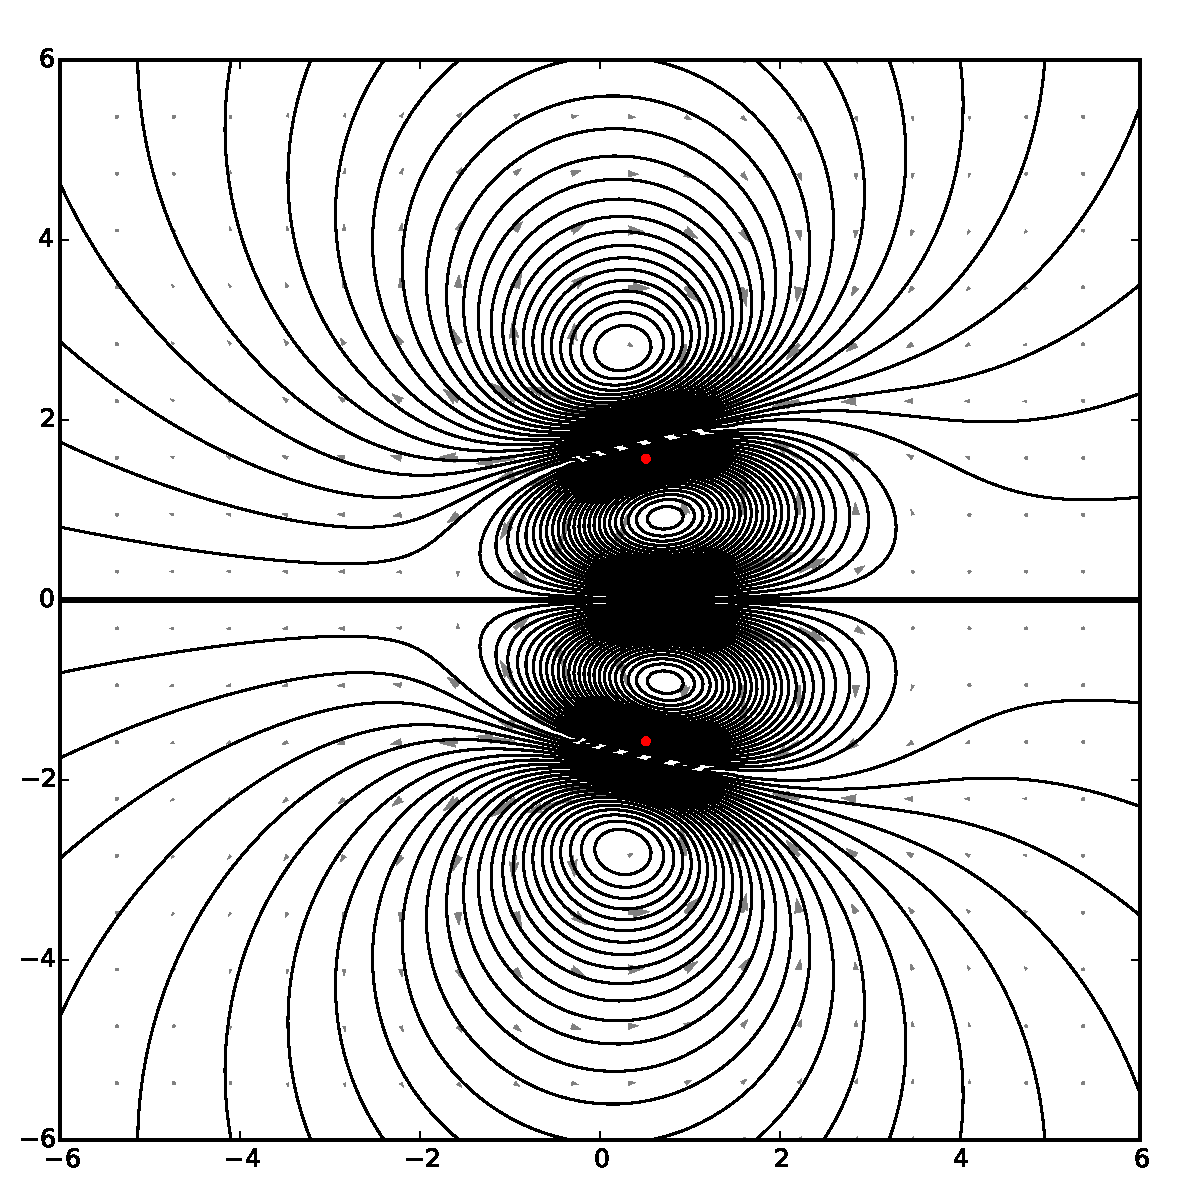
\includegraphics[width=0.3\textwidth]{./images/moi_frames/time_5}
	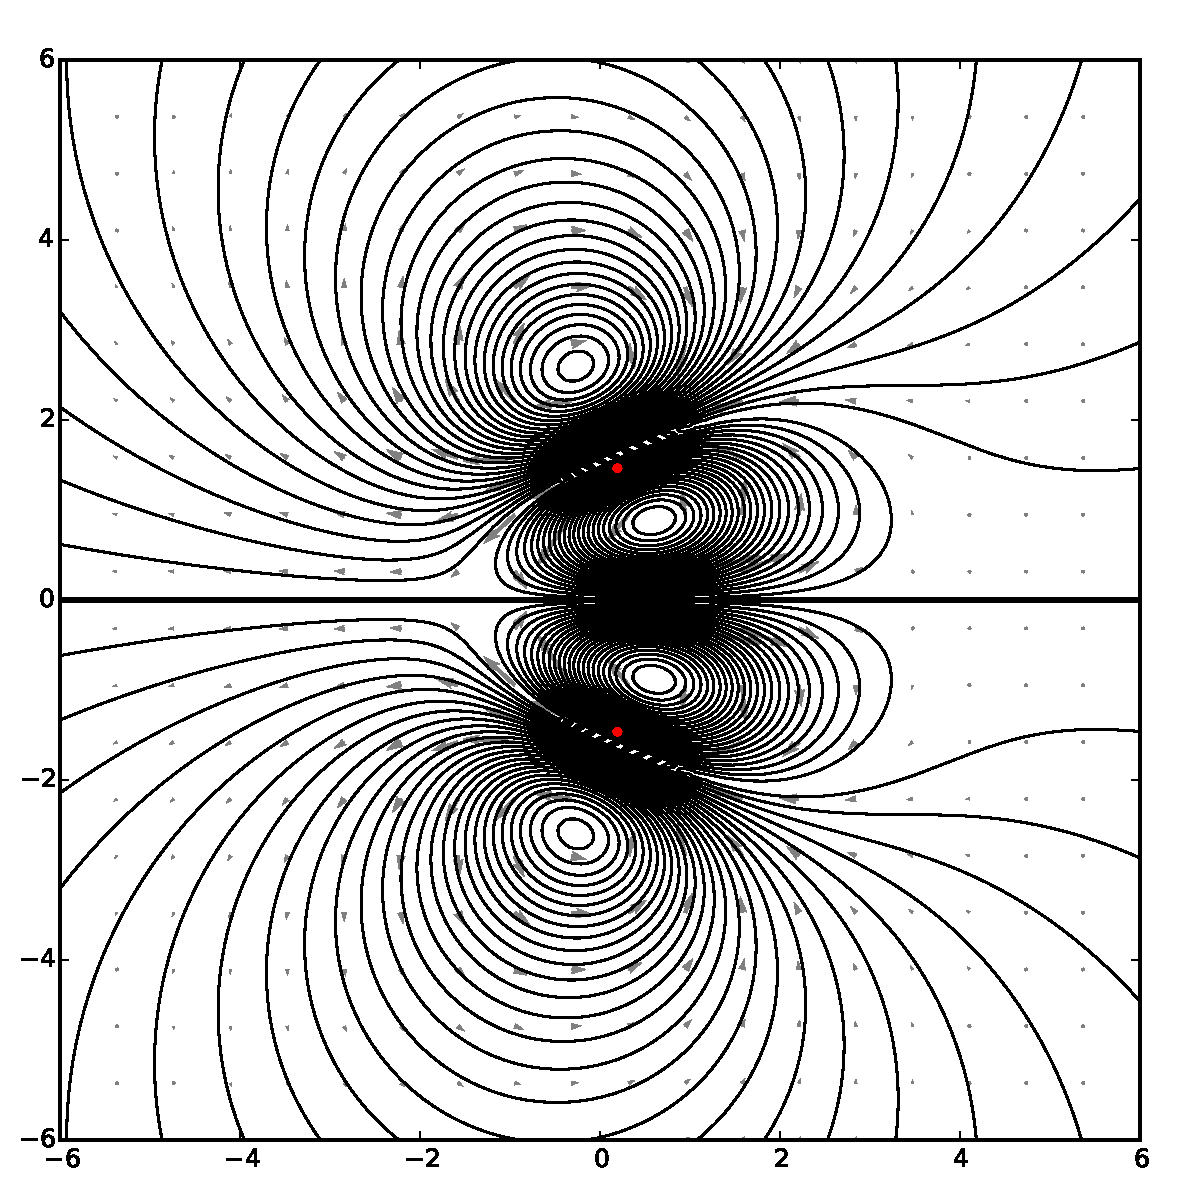
\includegraphics[width=0.3\textwidth]{./images/moi_frames/time_6p7}
	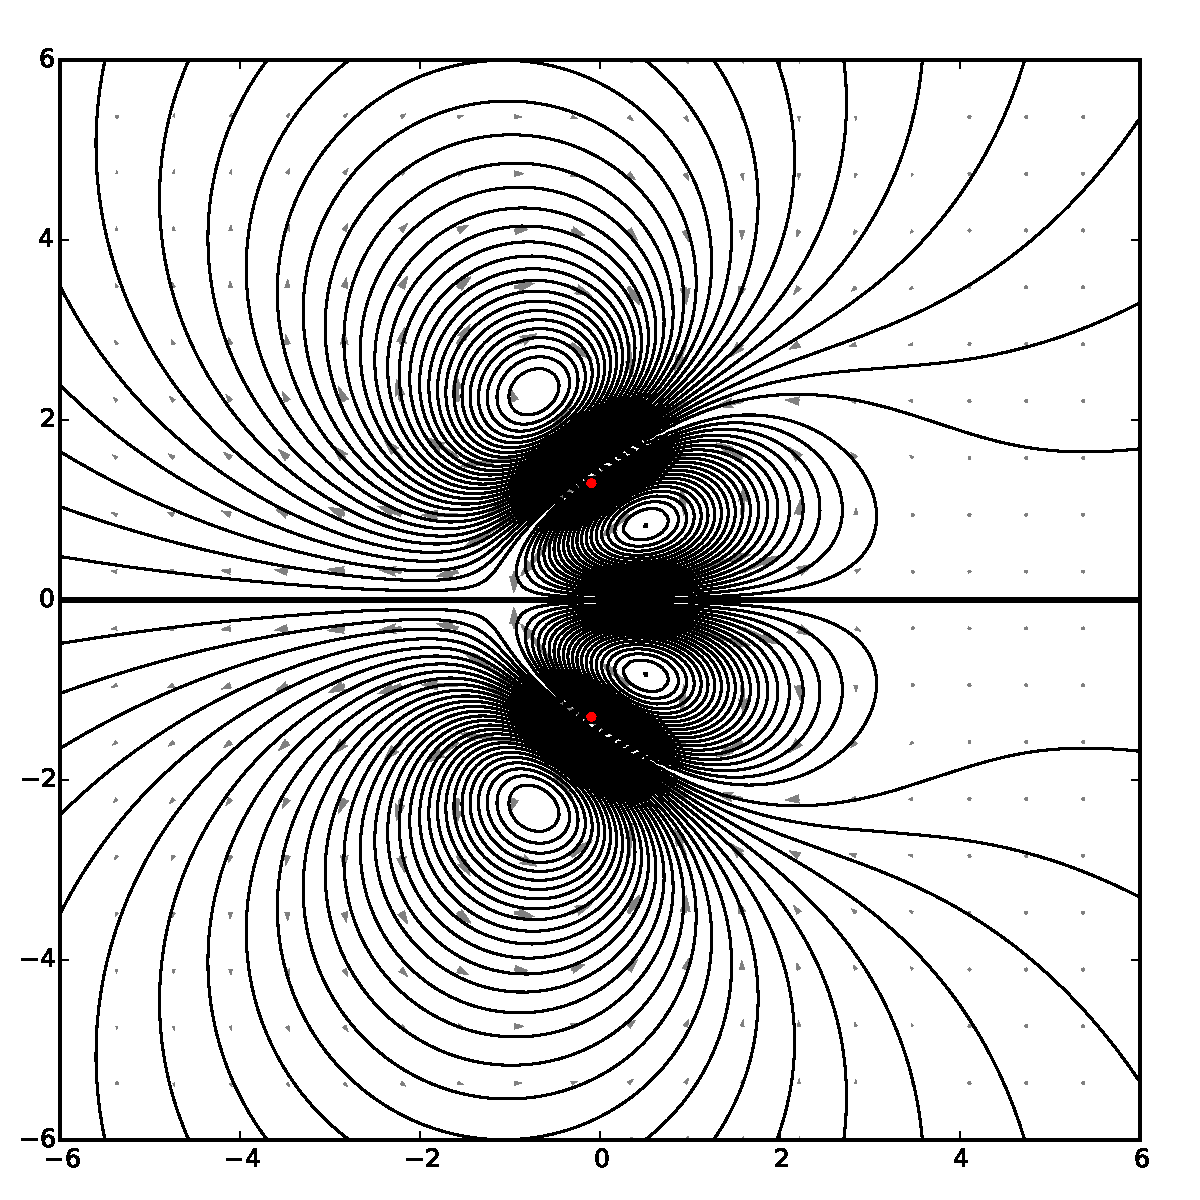
\includegraphics[width=0.3\textwidth]{./images/moi_frames/time_8p4}
	\caption{Numerical results are shown for two first order jet vortices with mirror-image initial conditions given by \eqref{eq:ic moi}.
		From left to right and top to bottom these are snapshots at times $t=0,1.7,3.4,5,6.7,8.4$ respectively. Apparently, a first order jet vortex reflects elastically from a fixed boundary, so that its angle of reflection equals its angle of incidence.}
	\label{fig:moi}
\end{figure}


\section{Hamiltonians and symplectic structures}
\label{sec:symplectic}
In modern Hamiltonian mechanics, as described in \cite{FOM,Arnold2000},
the Hamiltonian is a function on a symplectic manifold, which produces equations of motion.
An important instance of a symplectic manifold is a coadjoint orbit (defined below).
In this section we compute the coadjoint orbit of a jet vortex
as well as the associated symplectic structure.
For a general vorticity distribution $\omega$, the Hamiltonian is the kinetic energy
\begin{align}
  H(\omega) = \frac{1}{2} \int \omega(z) G_\delta(z-\tilde{z}) \omega(\tilde{z}) dz d\tilde{z}. \label{eq:Hamiltonian}
\end{align}
Where $\omega$ may be of the form \eqref{eq:ansatz N}.

The coadjoint orbit of $\omega$ is the set
\begin{align*}
  \Orb(\omega) := \{ \omega \circ \varphi^{-1} \mid \varphi \in \SDiff(\R^2) \}.
\end{align*}
%where $\varphi_* \omega$ denotes the distribution defined by
%\begin{align*}
%	\int f(z) (\varphi_*\omega)(z) := \int f(\varphi(z)) \omega(z) \,,\quad \quad \forall f \in C^\infty(\R^2).
%\end{align*}
In fact $\Orb(\omega)$ inherits the structure of a smooth manifold,
and a tangent vector on $\Orb(\omega)$ at the point $\tilde{\omega} \in \Orb(\omega)$ is given by 
a distribution denoted as $\pounds_{\vec{u}}[\tilde{\omega}] := u \partial_x \tilde{\omega} + v \partial_y \tilde{\omega}$ for some (non-unique) divergence free vector field
$\vec{u} = (u,v) \in \mathfrak{X}_{\rm div}(\R^2)$.
The symplectic structure is nothing more than a special case of the one derived via the Kirillov-Kostant-Souriau theorem \cite[see the boxed formula on p.303]{FOM}.
In particular, the symplectic structure on $\Orb(\omega)$ is given by
\begin{align}
  \Omega_\omega( \pounds_{\vec{u}_1}[\omega] , \pounds_{\vec{u}_2}[\omega] ) = \int \omega(z)  ( u_1(z) v_2(z) - v_1(z) u_2(z) ) dz. \label{eq:symplectic}
\end{align}
When $\omega$ is a smooth distribution, the symplectic structure may be identified with a differential $2$-form and this formula matches the symplectic form derived on page 313 of \cite{MarsdenWeinstein1983}.
In the case that $\omega$ satisfies the ansatz \eqref{eq:ansatz N}, we find that $\Orb(\omega)$ may be parametrized finite dimensionally in the following theorem.

\begin{thm}
	Let $\omega_0 = \gamma_i^\alpha \partial_{\alpha} \delta_{Z_i}$ for $\gamma_i^\alpha \neq 0$ and let
	$M^{(k)} = \{ \sum_{|\alpha| \leq k} \Gamma_i^\alpha \partial_{\alpha} \delta_{Z_i} \}$ be the space of $k$th order jet vortices.
	Then $\Orb(\omega_0)$ is a sub-manifold of the $M^{(k)}$.
\end{thm}
\begin{proof}
	Let $\varphi \in \SDiff(\R^2)$.  By applying the change of variables formula
	and noting that $\det(D\varphi)=1$, we find
	\begin{align*}
		\int \omega_0(\varphi^{-1}(z)) f(z) dz &= \int \omega_0(z) , f (\varphi(z)) dz \\
                &= \gamma_i^\alpha \partial_{\alpha}|_{z=Z_i} (f \circ\varphi)(z).
	\end{align*}
	By the multivariate Fa\'a di Bruno formula, the expression $\partial_{\alpha}|_{z=Z_i} (f \circ\varphi)(z)$
	is a sum of the partial derivatives of $f$ at the points $\varphi(Z_i)$
	of order less than that of the multi-index $\alpha$ \cite{ConstantineSavits1996}.
        Thus $ \omega_0 \circ \varphi^{-1} \in M^{(k)}$.
\end{proof}

Finally, as a check, we can also prove that the equations of motion are identical to the equations of motion obtained using this symplectic structure.

\begin{thm}
	Let $H(\omega)$ be given by \eqref{eq:Hamiltonian}.  Then Hamilton's equations on $\Orb(\omega_0)$
	are given by
	\begin{align*}
		\partial_t \omega + \partial_y \psi \partial_x \omega - \partial_x \psi \partial_y \omega \quad,\quad  \psi = G_\delta*\omega.
	\end{align*}
\end{thm}
\begin{proof}
  Let $\omega \in \Orb(\omega_0)$, and let $X_H(\omega) =  \pounds_{\vec{u}}[\omega]$ for some (non-unique) $\vec{u} = (u,v) \in \mathfrak{X}_{\rm div}(\R^2)$.
  Our goal is to solve for $\vec{u}$.
  By the definition of $X_H$ we see that for any
  $\vec{u}' = (u',v') \in \mathfrak{X}_{\rm div}(\R^2)$
  \begin{align*}
    \int \omega(z) \left( u(z) v'(z)  - v(z) u'(z) \right) dz &=
    \Omega_{\omega}( \pounds_{\vec{u}}[\omega] , \pounds_{\vec{u}'}[\omega] ) = - \int \frac{\delta H}{\delta \omega} (z) \left( \pounds_{\vec{u}'}[\omega] \right)(z) dz  \\
    &= - \int G_\delta(z-\tilde{z}) \omega (\tilde{z}) \left( \pounds_{\vec{u}'}[\omega] \right)(z) d\tilde{z} dz .
  \end{align*}
  If we let $\psi := G_\delta*\omega = \int G_\delta(\cdot -\tilde{z}) \omega (\tilde{z}) d \tilde{z}$ then integration by parts implies
  \begin{align*}
     \int \omega(z) \pounds_{\vec{u}'}[\psi](z) 
    =  \int \omega(z)  \left( u'(z) \partial_x \psi (z)+ v'(z) \partial_y \psi(z) \right) dz.
  \end{align*}
  We see that $\vec{u} = (-\partial_y \psi,\partial_x \psi)$ is one possible solution.
  As $\Omega$ is non-degenerate on the tangent spaces of $\Orb(\omega)$, this is the unique solution.
\end{proof}

\subsection{The first order case}
Let us illustrate these Hamiltonian results for the case of the first order jet vortex.
\begin{thm}
Let $z_1,\dots,z_n \in \R^2$ be distinct.
The coadjoint orbit of
\begin{align*}
  \omega = \sum_{i=1}^N \gamma_i \delta_{z_i} + \gamma_i^x \partial_x \delta_{z_i} + \gamma_i^y \partial_{y} \delta_{z_i}
\end{align*}
is
\begin{align*}
  \Orb(\omega) &= \left\{ \sum_{i=1}^n \gamma_i \delta_{z_i} + \Gamma_i^x \partial_x \delta_{\tilde{z}_i} + \Gamma_i^y \partial_{y} \delta_{z_i}
  \mid z_i \in \R^2, (\Gamma_i^x,\Gamma_i^y) \in \R^2 \backslash \{0\} \right\} \\
  &\cong  \{ (z_1,\dots,z_n,\Gamma_1,\dots,\Gamma_n) \mid z_i \in \R^2, \Gamma_i \in \R^2 \backslash \{0\} , ( i \neq j \implies z_i \neq z_j ) \}.
\end{align*}
The symplectic structure is
  \begin{align}
  \begin{split}
    \Omega( (\dot{z},\dot{\Gamma}), (\delta z,\delta \Gamma) ) &=
    \gamma_i ( \dot{x}_i \cdot \delta y_i - \delta x_i \cdot \dot{y}_i ) \\
    &\quad + \dot{\Gamma}_i^x \cdot \delta y_i
    - \dot{\Gamma}_i^y \cdot \delta x_i
    + \delta \Gamma_i^y \cdot \dot{x}_i 
    - \delta \Gamma_i^x \cdot \dot{y}_i
    \end{split} \label{eq:first_order_symplectic}
  \end{align}
\end{thm}

\begin{proof}
  Let $\omega$ be as above and consider some $\varphi \in \SDiff(\R^2)$.
  We find that for any function $f$
  \begin{align*}
    \int \omega \left(\varphi^{-1}(z)\right) f(z)dz &:= \int \omega (z)f\left(\varphi(z)\right) dz \\
    &= \gamma_i f(\varphi(Z_i)) \\
    &\quad - \gamma_i^x \partial_x \varphi^x|_{z=Z_i} \partial_x f |_{z=\varphi(Z_i)}
    - \gamma_i^x \partial_x \varphi^y|_{z=Z_i} \partial_y f |_{z=\varphi(Z_i)} \\
    &\quad - \gamma_i^y \partial_y \varphi^x|_{z=Z_i} \partial_x f |_{z=\varphi(Z_i)}
    - \gamma_i^y \partial_y \varphi^y|_{z=Z_i} \partial_y f |_{z=\varphi(Z_i)}
  \end{align*}
  Collecting like terms we find
  \begin{align*}
    \omega \circ \varphi^{-1} = \gamma_i \delta_{\varphi(Z_i)} + \Gamma_i^x \partial_x \delta_{\varphi(Z_i)} + \Gamma_i^y \partial_y \delta_{\varphi(Z_i)}
  \end{align*}
  where
  \begin{align*}
    \Gamma = 
    \begin{bmatrix}
      \Gamma_i^x \\ \Gamma_i^y 
    \end{bmatrix}
    =
    D\varphi(Z_i) \cdot
    \begin{bmatrix}
      \gamma_i^x \\ \gamma_i^y
    \end{bmatrix}
  \end{align*}
  By varying $\varphi$ we can obtain 
  any collection of distinct points $z_1,\dots,z_n \in \R^2$
  and any collection of non-zero vectors $\Gamma_1,\dots,\Gamma_n \in \R^2 \backslash \{0\}$.
  This proves the first claim.

  To derive the symplectic structure recall the symplectic structure for a general vorticity \eqref{eq:symplectic}.
  Now let $\omega = \gamma_i \delta_{z_i} + \Gamma_i^x \partial_x\delta_{z_i} + \Gamma_i^y \partial_y \delta_{z_i}$.
  In this case the left hand side of \eqref{eq:symplectic} can be computed with respect to 
  divergence free vector field $\vec{u} = (u,v)$ and $\vec{u}' = (u',v')$ as
  \begin{align*}
    \int \omega(z) \left( u v' - v u' \right) (z) dz &= \gamma_i ( u(z_i)v'(z_i) - v(z_i) u'(z_i) ) \\
    &\quad + \Gamma_i^x ( u_{,x} v' + u {v'}_{,x} - {u'}_{,x}v - u' v_{,x})|_{z = z_i} \\
    &\quad + \Gamma_i^y ( u_{,y} v' + u {v'}_{,y} - {u'}_{,y}v - u' v_{,y})|_{z = z_i}
  \end{align*}
  Note that this is written entirely in terms of the 1st order Taylor expansion of $\vec{u}$ and $\vec{u}'$ evaluated 
  at $z_i$.
  Moreover, $\pounds_{\vec{u}}[\omega] = \gamma_0 u(z_i) \partial_x \delta_{z_i} + \dots$
  also has the property that it only depends on
  the one-jet of $u$ and $v$ at the points $z_1,\dots,z_n$.
  Therefore, both sides of \eqref{eq:symplectic}
  can be written as a function of the finite collection of 
  numbers $u(z_i), Du(z_i), v(z_i),Dv(z_i)$.
  The result then follows by identifying the scalars
  \begin{align*}
    u(z_i) \mapsto u_{z_i}\\
    u^x_{,x}(z_i) \Gamma^x_i + u^x_{,y}(z_i) \Gamma^y_i \mapsto \dot{\Gamma}_i^x \\
    u^y_{,x}(z_i) \Gamma^x_i + u^y_{,y}(z_i) \Gamma^y_i \mapsto \dot{\Gamma}_i^y.
    \end{align*}
    with those which appear in \eqref{eq:first_order_symplectic}.
\end{proof}

\begin{rmk}
  The use of this symplectic structure shows that the map $(z_i, \Gamma_i,\Gamma_i^x,\Gamma_i^y) \mapsto \omega \in \Orb(\omega)$ is a symplectic momentum map.
\end{rmk}

\begin{rmk}
The corresponding Poisson bracket is given in tabular form by\\
\begin{center}
\begin{tabular}{|c|c|c|c|c|c|}
\hline
	$\{ \cdot , \cdot \}$ & $x$ & $y$ & $\Gamma$ & $\Gamma^x$  & $\Gamma^y$ \\ \hline
	$x$ & 0 & 1 & 0 & 0 & 1 \\ \hline
	$y$ & -1 & 0 & 0 & -1 & 0 \\ \hline 
	$\Gamma$ & 0 & 0 & 0 & 0 & 0 \\ \hline
	$\Gamma^x$ & 0 & -1 & 0 & 0 & 1 \\ \hline
	$\Gamma^y$ & 1 & 0 & 0 & -1 & 0  \\ \hline
\end{tabular}
\end{center}
\end{rmk}

\section{Conclusion}
\label{sec:Conclusion}
In this paper we have considered a generalization of the standard vortex blob method, obtained 
by augmenting the vortices with higher-order circulation variables
and dubbing them ``jet vortices''.
By viewing the vorticity equation as an advection equation, we have obtained equations of motion for these jet vortices.

The extra degrees of freedom of jet vortices resulted in richer dynamics near the vortex core.
Moreover, these new vortices exhibited a variety of interesting types of solution behavior.
We also observed faster convergence rates in space using higher order jet vortices.
Moreover, we proposed a scheme to decrease the number of pairwise interactions, by grouping
jet vortices of lower order into a smaller number of jet vortices of higher order.
Lastly, the implications of Kelvin's circulation theorem were substantially richer in the case of jet vortices, than for the 0-jet point vortices.

We have demonstrated the behavior of the jet vortices with a sequence of simple numerical experiments consisting of small numbers of jet vortices of various degrees.
We found 1st order jet vortices correspond to vortex dipoles which simply propagate themselves forward, while the 2nd order circulation variables activated richer (non-propagating) dynamics near the vortex core.

Finally, we derived the symplectic structure of jet vortices using methods from  \cite{MarsdenWeinstein1983}.
The resulting structure turned out to be a direct generalization of the standard
symplectic structure for vortex blobs.

Future avenues of inquiry could include:
\begin{itemize}
	\item jet vortex filament methods for $3$ dimensional fluid modelling
	\item jet vortices on manifolds, such as the sphere
	\item The convergence properties of the jet vortex method
\end{itemize}

\section{Acknowledgements}
Both authors gratefully acknowledge partial support by the European Research
Council Advanced Grant 267382 FCCA to DDH.

\appendix

\section{Distributions}
\label{sec:distributions}
The vorticity, $\omega$, should be viewed as a distribution
and the term ``$\partial_x \omega$'' should be viewed
as a distributional derivative.
When $\omega \in D(\R^2)$ is a smooth distribution there is little harm in naively interpreting $\omega$ as a smooth function on $\R^2$.
However, when $\omega$ is not smooth (e.g. a Dirac delta distribution),
then one needs to invoke the mathematics of distributions
as distinct from that of real valued functions.
Therefore, we have included this appendix to remind the reader of the basic theory of distributions.
The main reference for this section is \cite{Hormander2003}.

The space of distributions $D(\R^2)$ is the dual-vector space to the space of smooth functions $C^\infty(\R^2)$.
Therefore a distribution is defined by how it maps functions to real numbers.
%Given a distribution $\omega \in D(\R^2)$ and a function $f \in C^\infty(\R^2)$,
%we use the notation $\langle \omega , f \rangle$ to denote the real number $\omega(f)$.
%In the main text we will often use the notation $\int \omega(z) f(z) dz$ to denote this as well
%because it is more common in the fluids literature.
%However, this notation fallaciously suggests that we may view distributions as functions,
%so we will drop its use here.

The distributional derivative of a given distribution $\omega \in D(\R^2)$ in the $i$th coordinate direction may be defined as the distribution $\partial_i \omega$ obtained by
\begin{align*}
	\int \partial_i \omega (z) f(z) dz = - \int \omega(z) \partial_i f (z) dz.
\end{align*}
For example, the Dirac-delta distribution, $\delta_0$, is defined as the unique distribution such that
\begin{align*}
	\int \delta_0(z) , f (z) dz = f(0) \,,\quad \quad \forall f \in C^\infty(\R^2).
\end{align*}
The distributional derivative, $\partial_i \delta_0$, is given by
\begin{align*}
	\int \partial_i \delta_0 (z) f(z) dz = -\partial_i f(0) \,,\quad \quad \forall f \in C^\infty(\R^2).
\end{align*}
Given a distribution $\omega \in D(\R^2)$ and a function $g \in C^\infty(\R^2)$ one can define the
distribution $g \, \omega$ as
\begin{align*}
	\int (g \, \omega)(z)  f(z) dz = \int \omega(z) g(z)f(z) dz \,,\quad \quad \forall f \in C^\infty(\R^2).
\end{align*}
For example, we find that $g \, \delta _0 = g(0) \delta_0$.
A slightly more involved example is given by the computation of $g\, \partial_i \delta_0$.
We find
\begin{align*}
	\int (g \, \partial_i \delta_0) (z)  f(z) dz = \int \partial_i \delta_0(z) g(z)f(z) dz =  - g(0) \partial_i f(0) - \partial_ig(0) f(0).
\end{align*}
Therefore
\begin{align*}
	g \, \partial_i \delta_0 = g(0) \partial_i \delta_0 - \partial_i g(0) \delta_0.
\end{align*}
On the left hand side, note that $g(0)$ and $\partial_i g(0)$ are merely real numbers,
which are multiplying the distributions $\partial_i \delta_0$ and $\delta_0$.
More generally, we find
\begin{align*}
	\int (g\, \partial_x^m \partial_y^n \delta_0)(z) f(z) dz &= (-1)^{m+n} \partial_x^m \partial_y^n (fg)(0) \\
		&= (-1)^{m+n} \sum_{\ell,k=0}^{m,n} \binom{m}{\ell} \binom{n}{k}
		\left(\partial_{x}^{\ell} \partial_y^k f(0) \right) 
		\left(\partial_{x}^{m-\ell} \partial_y^{n-k} g(0) \right) 
\end{align*}
which means
\begin{align}
	g \, \partial_x^m \partial_y^n \delta_0 =
		(-1)^{m+n} \sum_{\ell,k=0}^{m,n} (-1)^{\ell + k}
		\binom{m}{\ell} \binom{n}{k}
		\left(\partial_{x}^{m-\ell} \partial_y^{n-k} g(0) \right) 
		\partial_{x}^{\ell} \partial_y^k \delta_0.
                \label{eq:func times partial delta}
\end{align}

%Let $L$ be the pseudo-differential operator dual to $G*$.
%Then $\langle \omega^{(0)}_h - \omega , f \rangle = \langle \psi - \psi_h^{(0)} , L[f] \rangle_{L^2}$,
%and the sup-norm of $\psi-\psi_h^{(0)}$ is order $o(1)$, so that the whole expression is $o(1)$
%for any $f$ in the RKHS produced by $G$.
%Then $\langle \omega^{(0)}_h - \omega , f \rangle = \langle \psi - \psi_h^{(0)} , L[f] \rangle_{L^2}$,
%and the sup-norm of $\psi-\psi_h^{(0)}$ is order $o(1)$, so that the whole expression is $o(1)$
%for any $f$ in the RKHS produced by $G$.
\section{Symmetries and Conserved Momenta}
\label{sec:symmetries}
Let $G$ be a Lie group with Lie algebra $\mathfrak{g}$.
We will denote the dual of $\mathfrak{g}$ by $\mathfrak{g}^*$.
A (left) group action of $G$ on a manifold $S$ is a map $\varrho: G \times S \to S$
such that $\varrho( g h , x) = \varrho(g , \varrho(h , x))$ for all $g,h, \in G$ and $x \in S$.
\begin{rmk}
The group action $\varrho$ is not to be confused with the fluid density, often denoted as $\rho$ in fluid mechanics.
This appendix relates to more general mathematical constructions which are useful, but not necessarily in the usual purview of fluid mechanics.
In particular, the symbol $\varrho$ is the Greek letter `r', and is used as a reference to the word ``representation''
as in ``representation theory''.
\end{rmk}
One can also construct a group action, $D\varrho: G \times TS \to TS$,  given by
$D\varrho( g , u ) := \left.\frac{d}{dt}\right|_{t=0} \rho(g, x(t) )$ for $u = \frac{dx}{dt} \in T_x S$ and $g \in G$.
There is also a natural Lie-algebra action, which one could also denote by $\varrho: \mathfrak{g} \times S \to TS$
defined by $\varrho( \xi , x) := \left. \frac{d}{d \epsilon} \right|_{\epsilon =0} \varrho( g_\epsilon , x)$.
In particular, the map $\varrho( \xi , \cdot ) : S \to TS$ is a vector-field on $S$ which we call the
\emph{infinitesimal generator} of $\xi$.
When no confusion arises, it is typical to use the notation $g \cdot x$, $g \cdot u$, and $\xi \cdot x$ to denote $\varrho(g,x)$,$D\varrho(g,u)$,  and $\varrho(\xi,x)$, respectively.
Finally, if $(S,\Omega)$ is a symplectic manifold, then we say that $G$ acts \emph{symplectically} (or \emph{canonically})
if $\Omega_{g \cdot x}( g \cdot u , g \cdot v) = \Omega_x(u,v)$ for all $g \in G$, $u,v \in T_x S$ and $x \in S$.

Let us now recall the notion of a momentum map \cite[Definition 4.2.1]{FOM}.
Given a symplectic manifold $(S,\Omega)$ and a Lie group $G$ which acts on $(S,\Omega)$ symplectically, a momentum map is a map ${\bf J}:S \to \mathfrak{g}^*$ such that
\begin{align*}
  d \langle {\bf J} , \xi \rangle = i_{\xi_S} \Omega\,,
\end{align*}
where $\langle {\bf J} , \xi \rangle$ denotes the real-valued function on $S$ obtained by pairing ${\bf J}$ with an arbitrary
 $\xi \in \mathfrak{g}$, and where $\xi_S \in \mathfrak{X}(S)$ is the infinitesimal generator of $\xi$ on $S$.
Equivalently, we could express the previous condition as
\begin{align}
  d \langle {\bf J},\xi \rangle(x) \cdot v_x = \Omega( \xi\cdot x , v_x ) \label{eq:momap}
\end{align}
for all $\xi \in \mathfrak{g}$, $x \in S$ and $v_x \in T_xS$.
Momentum maps are significant for a number of reasons.
In particular, given a Hamiltonian on $S$ with $G$-symmetry, the momentum map ${\bf J}$ will be conserved under the evolution of
Hamilton's equations \cite[Theorem 4.2.2]{FOM}.
This is nothing but the Hamiltonian version of Noether's theorem.

In our case $S = {\rm Orb}(\omega_0) = \{ \omega_0 \circ \varphi^{-1} \mid \varphi \in \SDiff(\mathbb{R}^2) \}$ is a coadjoint orbit of some vorticity distribution on $\mathbb{R}^2$.
Tangent vectors on $S$ are of the form $$\pounds_{\vec{u}} [\omega] := u \partial_x \omega + v \partial_y \omega$$ for a (perhaps non-unique) divergence free vector-field $\vec{u} = (u,v)$.
Under this identification, the symplectic form at some $\omega \in S$ is given by an application of Kostant's formula \cite{FOM}.
This is derived in section \ref{sec:symplectic} and found to be
\begin{align*}
  \Omega_\omega( \pounds_{\vec{u}_1}[\omega] , \pounds_{\vec{u}_2} [\omega] ) :=
  \int \omega(z) ( \vec{u}_1(z) \times \vec{u}_2(z) ) dz.
\end{align*}
where $\vec{u}_1$ and $\vec{u}_2$ are divergence free vector-fields and $\times$ denotes the planar cross product.
Here we interpret the planar cross product as taking values in the space of real-numbers so that $\vec{u}_1 \times \vec{u}_2$ is
merely a smooth function.

We now will translate formula \eqref{eq:momap} to this more specific scenario.
Assume $G$ acts upon $\mathbb{R}^2$, then $G$ also acts upon distributions and upon $S$ by symplectic group actions.
In this context, a momentum map ${\bf J}$ associated to a $G$-action is defined by the equation
\begin{align}
  \int \frac{\delta  \langle {\bf J} , \xi \rangle }{\delta \omega} (z)  \left( \pounds_{\vec{u}}[\omega] \right)(z) dz = \int \omega(z)  \left( (\xi \cdot z) \times \vec{u}(z) \right)dz \label{eq:momap2}
\end{align}
Where $\xi \cdot z$ denotes the action of $\xi \in \mathfrak{g}$ on $z \in \R^2$
and ``$\times$'' denotes the planar cross-product.

\subsection{Translational symmetry and ${\bf J}_{\rm lin}$}
%In this section we consider the action of translation in $\R^2$.
%This action on $\R^2$ will induce a symplectic group action on the symplectic manifold $S = {\rm Orb}(\omega_0)$ derived in \S \ref{sec:symplectic}.

The group $\mathbb{R}^2$ acts upon $\mathbb{R}^2$ by translation.
That is to say, by sending any $\tilde{z} \in \R^2$ to $z + \tilde{z} \in \R^2$ for any $\tilde{z}  \in \R^2$.
This fact induces an action on smooth functions.
In particular, there is a natural (right) action on $C^{\infty}(\mathbb{R}^2)$ sending the function $\phi(z)$ to the function  $(\tilde{z})^*\phi(z) := \phi(z-\tilde{z})$.
We denote the inverse operation by $(\tilde{z})_* \phi(z) := \phi( z + \tilde{z})$.
This induces a (left) action on distributions which sends $\omega \in \mathcal{D}'(\R^2)$ to the distribution $(\tilde{z})_*\omega(z) := \omega( z +\tilde{z})$.
As a translation of $\mathbb{R}^2$ by $\tilde{z}$ is a volume-preserving diffeomorphism, we see that the coadjoint orbit $S \subset \mathcal{D}(\mathbb{R}^2)$ is invariant under this action.
Moreover, we observe the action, restricted to $S$, is symplectic because
\begin{align*}
  \Omega_{ \tilde{z}_* \omega}( \tilde{z}_*\pounds_{u}[ \omega] , \tilde{z}_*\pounds_v[\omega] ) &= \Omega_{\tilde{z}_* \omega} ( \pounds_{\tilde{z}_*u}[ \tilde{z}_*\omega] ,
  \pounds_{\tilde{z}_*v}[\tilde{z}_*\omega] ) \\
  &= \int \tilde{z}_* \omega(z)  \left( \tilde{z}_*(u \times v) \right)(z) dz \\
  &= \int \omega( z+\tilde{z}) \left(u \times v \right)(z + \tilde{z}) dz \\ 
  &= \int \omega(z) \left( u \times v \right)(z) dz  \\
  &= \Omega_{\omega}( \pounds_u[\omega], \pounds_v[\omega]).
\end{align*}

Given this symplectic action, we can seek a momentum map, ${\bf J}_{\rm lin}:S \to (\mathbb{R}^2)^*$.  Consider an arbitrary element of the Lie-algebra $\delta \tilde{z}  = (\delta \tilde{x}, \delta \tilde{y}) \in \mathbb{R}^2$ and use \eqref{eq:momap2} to obtain
\begin{align*}
  \int \frac{\delta \langle {\bf J}_{\rm lin} , \delta \tilde{z} \rangle}{\delta \omega}(z)   \pounds_{\vec{u}}[\omega] dz
  = \int \omega(z) \left( \delta \tilde{x} \, v(z) - \delta \tilde{y} \, u(z) \right) dz
\end{align*}
We can re-write the right hand side as
\begin{align*}
  = \int \omega(z)  \pounds_{\vec{u}} [ \delta \tilde{x} \, y - \delta \tilde{y} \, x] dz
\end{align*}
and upon integrating by parts this is equivalent to
\begin{align*}
  = - \int \pounds_{\vec{u}}[\omega](z)  \left( \delta \tilde{x}\, y - \delta \tilde{y}\, x \right) dz
\end{align*}
Therefore, ``cancelling'' the arbitrary vector $\pounds_v[\omega]$ from both sides we find
\begin{align*}
  \frac{\delta  \langle {\bf J}_{\rm lin} , \delta \tilde{z} \rangle}{\delta \omega} = \delta \tilde{y} x - \delta \tilde{x} y
\end{align*}
Integrating by $\omega$ we find
\begin{align*}
  \boxed{
    {\bf J}_{\rm lin}(\omega) = \left( -\int \omega(z) y dz \, , \, \int \omega(z) x dz \right) \in (\mathbb{R}^2)^* \equiv \mathbb{R}^2}
\end{align*}
If $\omega$ satisfies the jet vortex ansatz
\begin{align*}
  \omega = \Gamma_i \delta_{z_i} + \Gamma_i^x \partial_x \delta_{z_i} + \Gamma_i^y \partial_y \delta_{z_i} + \dots
\end{align*}
then
\begin{align*}
  {\bf J}_{\rm lin}(\omega) = \sum_i ( \Gamma_i^{y} - \Gamma_i y_i , \Gamma_i x_i -\Gamma_i^{x} ).
\end{align*}
The terms of the jet vortices beyond the first order do not influence ${\bf J}_{\rm lin}$.

\subsection{Rotational symmetry and ${\bf J}_{\rm ang}$}
The group $\SO(2)$ acts upon $\mathbb{R}^2$ by rotations about the origin sending $z \in \R^2$ to $R_\theta \cdot z := ( \cos(\theta)x-\sin(\theta)y,\sin(\theta)x+\cos(\theta)y )$.
For any $\theta \in \SO(2)$, there is a natural action on $C^{\infty}(\mathbb{R}^2)$ sending the function $\phi \in C^{\infty}(\mathbb{R}^2)$ to the function $\theta^*\phi(x,y) := \phi(\cos(\theta)x-\sin(\theta)y,\sin(\theta)x+\cos(\theta)y)$.  The corresponding action on vector-fields and all other objects on $\mathbb{R}^2$ follows naturally.  
 In particular, the left-action on distributions sends $\omega \in \mathcal{D}'(\mathbb{R}^2)$ to the distribution $\theta_* \omega(z) := \omega( R_\theta \cdot z)$.
Again, we can verify that the coadjoint orbit $S$ is invariant under this action, and that $\SO(2)$ acts symplectically upon $S$
through computations which are analogous to those performed in the previous subsection.
Given this symplectic action, we can seek a momentum map, ${\bf J}_{\rm ang}:S \to \mathfrak{so}(2)^* \equiv \mathbb{R}$.  Consider an arbitrary element of the Lie-algebra $\xi \in \mathfrak{so}(2) \equiv \mathbb{R}$ and use \eqref{eq:momap2} to obtain
\begin{align*}
  \int  \frac{\delta  \langle {\bf J}_{\rm ang} (z) , \xi \rangle }{\delta \omega} (z) \, \pounds_{\vec{u}}[\omega] (z) dz
  = \int \omega(z) \left( -y\xi v - x\xi u \right) dz
\end{align*}
We can re-write the right hand side and integrate by parts to find
\begin{align*}
  = -\xi \int \omega(z) \pounds_{\vec{u}} \left[\frac{x^2+y^2}{2}\right] dz
  = \xi \int \pounds_{\vec{u}}[\omega](z) \left( \frac{x^2+y^2}{2} \right) dz.
\end{align*}
As the vector $\pounds_{\vec{u}}[\omega] \in T_\omega S$ is arbitrary we find
\begin{align*}
  \frac{\delta \langle {\bf J}_{\rm ang} , \xi \rangle}{\delta \omega} = \xi \frac{x^2+y^2}{2}
\end{align*}
Integrating by $\omega$ we find
\begin{align*}
  \boxed{
    {\bf J}_{\rm ang}(\omega) = \frac{1}{2}\int \omega(z) ( x^2 + y^2) dz \in \mathbb{R} \equiv \mathfrak{so}(2)^*
    }
\end{align*}
If $\omega$ satisfies the jet vortex ansatz
\begin{align*}
  \omega = \Gamma_i \delta_{z_i} + \Gamma_i^x \partial_x \delta_{z_i} + \Gamma_i^y \partial_y \delta_{z_i} + \Gamma_i^{xx} \partial_{xx} \delta_{z_i} + \dots
\end{align*}
then
\begin{align*}
  {\bf J}_{\rm ang}(\omega) = \frac{\Gamma_i}{2} (x_i^2 + y_i^2) - \Gamma_i^x x_i - \Gamma_i^y y_i + \Gamma_i^{xx} + \Gamma_i^{yy} .
\end{align*}
The terms of the jet vortices beyond the second order do not influence the angular momentum ${\bf J}_{\rm ang}$.

%\begin{thebibliography}{}
%
%\bibitem{Chen-etal1999} Chen-etal1999
%
%\bibitem{Ch1972} A. J. Chorin, Vortex methods for rapid flow, Proc. 2d Int. Cong. Num. Meth. Fluid
%Mech., Springer, 1972.
%
%\bibitem{Ch1973}  A. J. Chorin, Numerical study of slightly viscous flow, J. Fluid Mech., 57, 785-796 (1973)
%
%\bibitem{Ch1980} A. J. Chorin, Vortex models and boundary layer instability, SIAM J. Sc. Stat.
%Comp., 1, 1-21 (1980).
%
%\bibitem{Ch1993} 
%A. J. Chorin [1993] Vortex Methods,
%Presented at Les Houches Summer School of Theoretical Physics
%Les Houches, France, June 28-July 30, 1993. DoE Report LBL-34124 Rev.
%
%\bibitem{Ch1993} A. J. Chorin, \textit{Vorticity and Turbulence}, Springer, 1993.
%
%\bibitem{ChBe1973} A. J. Chorin and P. Bernard, discretization of a vortex sheet with an example of roll-up, J. Comp. Phys., 13, 423-429 (1973).
%
%\bibitem{CoKo2000}
%G.-H. Cottet and P. Koumoutsakos [2000] \textit{Vortex Methods: Theory and Practice}, Cambridge Univ. Press, Cambridge, UK.
%
%\bibitem{EbMa1970} Ebin and Marsden 1970
%
%\bibitem{FoHoTi2001} FoHoTi2001 Physica D
%
%\bibitem{FoHoTi2002} FoHoTi2002 Dyn Sys 
%
%\bibitem{Geurts-etal200X} Geurts-etal200X
%
%\bibitem{GjajaHolm1996} GjajaHolm1996
%
%\bibitem{Hecht-etal200Z} Hecht-etal200Z
%
%\bibitem{Ho2001} Ho2001 Physica D paper
%
%\bibitem{Ho2002} Ho2002 Chaos paper
%
%\bibitem{HoMaRa1998} HoMaRa 1998 AIM Paper
%
%\bibitem{HoRaTrYo2005}
%Darryl D. Holm, J. Tilak Ratnanather, Alain Trouv\'e, Laurent Younes [2004]
%Soliton dynamics in computational anatomy,
%NeuroImage, 23 (S1): S170--S178.
%
%\bibitem{Kr1986} R. Krasny, A study of singularity formation in a vortex sheet by the point vortex
%approximation, J. Fluid Mech., 167, 65-93 (1986)
%
%\bibitem{LANSalphaRefs} LANS-alpha Refs, 
%\begin{description}
%\item Gjaja and Holm
%\item Holm \textit{Chaos} and \textit{Physica D}
%\item Chen et al.
%\item Marsden and Shkoller
%\item FoHoTi2001 Physica D and FoHoTi2002 Dyn Syst
%\item Geurts et al.
%\item Fried et al.
%\item Rebholtz
%\item Pouquet et al.
%\item Hecht et al. 
%\end{description}
%
%
%\bibitem{Le1975} A. Leonard, Numerical simulation of interacting three-dimensional vortex filaments, Proc. 4th Int. Conf. Num. Meth. Fluids, Springer, 1975
%
%%\bibitem{Le1980}
%%A. Leonard [1980] Vortex methods for flow simulation, J. Comput. Phys. 37 (3): 289.
%
%\bibitem{Le1985} A. Leonard, Computing three dimensional vortex flows with vortex filaments, Ann. Rev. Fluid Mech., 17: 523-559 (1985)
%
%\bibitem{MaSh2002} Marsden and Shkoller, Phil Trans Roy Soc ??
%
%\bibitem{MiMu2014} Michor Mumford JGM 2014
%
%\bibitem{Newton} Paul Newton's book, \textit{The $N$-Vortex Problem}
%
%\bibitem{Pouquet-etal200Y} Pouquet-etal 200Y
%
%\bibitem{Ro1931} L. Rosenhead, The formation of vortices from a surface of discontinuity, Proc. Roy. Soc. London, A 134: 170-192 (1931)
%
%\bibitem{Saffman} Phil Saffman's book, \textit{Vorticity}
%
%\bibitem{Sa1989}
%T. Sarpkaya [1989] Computational methods with vortices�The 1988 Freeman Scholar Lecture, J. Fluids Eng. 111: 5.
%
%\bibitem{Stock2007} M. J. Stock, Summary of Vortex Methods Literature
%(A living document rife with opinion), Online at \url{http://markjstock.org/research/vortex_methods_literature.pdf}
%
%\bibitem{TrVi2012} A. Trouv\'e, F. X. Vialard [2012] Shape splines and stochastic shape evolutions: a second order point of view, Quart. Appl. Math 70: 219�251.
%
%\end{thebibliography}

\bibliographystyle{amsalpha}
\bibliography{hoj_2015}

\end{document}
